% This is the Reed College LaTeX thesis template. Most of the work
% for the document class was done by Sam Noble (SN), as well as this
% template. Later comments etc. by Ben Salzberg (BTS). Additional
% restructuring and APA support by Jess Youngberg (JY).
% Your comments and suggestions are more than welcome; please email
% them to cus@reed.edu
%
% See https://www.reed.edu/cis/help/LaTeX/index.html for help. There are a
% great bunch of help pages there, with notes on
% getting started, bibtex, etc. Go there and read it if you're not
% already familiar with LaTeX.
%
% Any line that starts with a percent symbol is a comment.
% They won't show up in the document, and are useful for notes
% to yourself and explaining commands.
% Commenting also removes a line from the document;
% very handy for troubleshooting problems. -BTS

% As far as I know, this follows the requirements laid out in
% the 2002-2003 Senior Handbook. Ask a librarian to check the
% document before binding. -SN

%%
%% Preamble
%%
% \documentclass{<something>} must begin each LaTeX document
\documentclass[12pt,oneside,a4paper]{reedthesis}
% Packages are extensions to the basic LaTeX functions. Whatever you
% want to typeset, there is probably a package out there for it.
% Chemistry (chemtex), screenplays, you name it.
% Check out CTAN to see: https://www.ctan.org/
%%
\usepackage{graphicx,latexsym}
\usepackage{amsmath}
\usepackage{amssymb,amsthm}
\usepackage{longtable,booktabs,setspace}
\usepackage{chemarr} %% Useful for one reaction arrow, useless if you're not a chem major
\usepackage[hyphens]{url}
% Added by CII
\usepackage[hidelinks]{hyperref}
\usepackage{lmodern}
\usepackage{float}
\floatplacement{figure}{H}
% Thanks, @Xyv
\usepackage{calc}
% End of CII addition
\usepackage{rotating}

% Next line commented out by CII
%%% \usepackage{natbib}
% Comment out the natbib line above and uncomment the following two lines to use the new
% biblatex-chicago style, for Chicago A. Also make some changes at the end where the
% bibliography is included.
%\usepackage{biblatex-chicago}
%\bibliography{thesis}
% \ifxetex
%   \usepackage{polyglossia}
%   \setmainlanguage{spanish}
%   % Tabla en lugar de cuadro
%   \gappto\captionsspanish{\renewcommand{\tablename}{Tabla}
%           \renewcommand{\listtablename}{Índice de tablas}}
% \else
%   \usepackage[spanish,es-tabla]{babel}
% \fi

% Added by CII (Thanks, Hadley!)
% Use ref for internal links
\renewcommand{\hyperref}[2][???]{\autoref{#1}}
\def\chapterautorefname{chapter}
\def\sectionautorefname{section}
\def\subsectionautorefname{subsection}
% End of CII addition

% Added by CII
\usepackage{caption}
\captionsetup{width=5in}
% End of CII addition

% \usepackage{times} % other fonts are available like times, bookman, charter, palatino

% Syntax highlighting #22
  \usepackage{color}
  \usepackage{fancyvrb}
  \newcommand{\VerbBar}{|}
  \newcommand{\VERB}{\Verb[commandchars=\\\{\}]}
  \DefineVerbatimEnvironment{Highlighting}{Verbatim}{commandchars=\\\{\}}
  % Add ',fontsize=\small' for more characters per line
  \usepackage{framed}
  \definecolor{shadecolor}{RGB}{248,248,248}
  \newenvironment{Shaded}{\begin{snugshade}}{\end{snugshade}}
  \newcommand{\AlertTok}[1]{\textcolor[rgb]{0.94,0.16,0.16}{#1}}
  \newcommand{\AnnotationTok}[1]{\textcolor[rgb]{0.56,0.35,0.01}{\textbf{\textit{#1}}}}
  \newcommand{\AttributeTok}[1]{\textcolor[rgb]{0.77,0.63,0.00}{#1}}
  \newcommand{\BaseNTok}[1]{\textcolor[rgb]{0.00,0.00,0.81}{#1}}
  \newcommand{\BuiltInTok}[1]{#1}
  \newcommand{\CharTok}[1]{\textcolor[rgb]{0.31,0.60,0.02}{#1}}
  \newcommand{\CommentTok}[1]{\textcolor[rgb]{0.56,0.35,0.01}{\textit{#1}}}
  \newcommand{\CommentVarTok}[1]{\textcolor[rgb]{0.56,0.35,0.01}{\textbf{\textit{#1}}}}
  \newcommand{\ConstantTok}[1]{\textcolor[rgb]{0.00,0.00,0.00}{#1}}
  \newcommand{\ControlFlowTok}[1]{\textcolor[rgb]{0.13,0.29,0.53}{\textbf{#1}}}
  \newcommand{\DataTypeTok}[1]{\textcolor[rgb]{0.13,0.29,0.53}{#1}}
  \newcommand{\DecValTok}[1]{\textcolor[rgb]{0.00,0.00,0.81}{#1}}
  \newcommand{\DocumentationTok}[1]{\textcolor[rgb]{0.56,0.35,0.01}{\textbf{\textit{#1}}}}
  \newcommand{\ErrorTok}[1]{\textcolor[rgb]{0.64,0.00,0.00}{\textbf{#1}}}
  \newcommand{\ExtensionTok}[1]{#1}
  \newcommand{\FloatTok}[1]{\textcolor[rgb]{0.00,0.00,0.81}{#1}}
  \newcommand{\FunctionTok}[1]{\textcolor[rgb]{0.00,0.00,0.00}{#1}}
  \newcommand{\ImportTok}[1]{#1}
  \newcommand{\InformationTok}[1]{\textcolor[rgb]{0.56,0.35,0.01}{\textbf{\textit{#1}}}}
  \newcommand{\KeywordTok}[1]{\textcolor[rgb]{0.13,0.29,0.53}{\textbf{#1}}}
  \newcommand{\NormalTok}[1]{#1}
  \newcommand{\OperatorTok}[1]{\textcolor[rgb]{0.81,0.36,0.00}{\textbf{#1}}}
  \newcommand{\OtherTok}[1]{\textcolor[rgb]{0.56,0.35,0.01}{#1}}
  \newcommand{\PreprocessorTok}[1]{\textcolor[rgb]{0.56,0.35,0.01}{\textit{#1}}}
  \newcommand{\RegionMarkerTok}[1]{#1}
  \newcommand{\SpecialCharTok}[1]{\textcolor[rgb]{0.00,0.00,0.00}{#1}}
  \newcommand{\SpecialStringTok}[1]{\textcolor[rgb]{0.31,0.60,0.02}{#1}}
  \newcommand{\StringTok}[1]{\textcolor[rgb]{0.31,0.60,0.02}{#1}}
  \newcommand{\VariableTok}[1]{\textcolor[rgb]{0.00,0.00,0.00}{#1}}
  \newcommand{\VerbatimStringTok}[1]{\textcolor[rgb]{0.31,0.60,0.02}{#1}}
  \newcommand{\WarningTok}[1]{\textcolor[rgb]{0.56,0.35,0.01}{\textbf{\textit{#1}}}}

% To pass between YAML and LaTeX the dollar signs are added by CII
\title{Dinámica de la circulación zonalmente asimétrica del hemisferio sur}
\author{Lic. Elio Campitelli}
% The month and year that you submit your FINAL draft TO THE LIBRARY (May or December)
\date{BUENOS AIRES, 2023}
\division{Facultad de Ciencias Exactas y Naturales}
\advisor{Dra. Carolina Vera}
\institution{Universidad de Buenos Aires}
\degree{Tesis presentada para optar al título de Doctor de la Universidad de Buenos Aires en el Área de Ciencias de la Atmósfera y los Océanos}
%If you have two advisors for some reason, you can use the following
% Uncommented out by CII
\altadvisor{Dr.~Leandro Diaz}
\consejere{Dr.~Claudio Menendez}
\place{Centro de Investigaciones del Mar y la Atmósfera. CONICET-UBA}
% End of CII addition

%%% Remember to use the correct department!
\department{Departamento de Ciencias de la Atmósfera y los Océanos}
% if you're writing a thesis in an interdisciplinary major,
% uncomment the line below and change the text as appropriate.
% check the Senior Handbook if unsure.
%\thedivisionof{The Established Interdisciplinary Committee for}
% if you want the approval page to say "Approved for the Committee",
% uncomment the next line
%\approvedforthe{Committee}

% Added by CII
%%% Copied from knitr
%% maxwidth is the original width if it's less than linewidth
%% otherwise use linewidth (to make sure the graphics do not exceed the margin)
\makeatletter
\def\maxwidth{ %
  \ifdim\Gin@nat@width>\linewidth
    \linewidth
  \else
    \Gin@nat@width
  \fi
}
\makeatother

\makeatletter
\renewcommand{\@chapapp}{Capítulo}
\makeatother

% From {rticles}
\newlength{\csllabelwidth}
\setlength{\csllabelwidth}{3em}
\newlength{\cslhangindent}
\setlength{\cslhangindent}{1.5em}
% for Pandoc 2.8 to 2.10.1
\newenvironment{cslreferences}%
  {}%
  {\par}
% For Pandoc 2.11+
% As noted by @mirh [2] is needed instead of [3] for 2.12
\newenvironment{CSLReferences}[2] % #1 hanging-ident, #2 entry spacing
 {% don't indent paragraphs
  \setlength{\parindent}{0pt}
  % turn on hanging indent if param 1 is 1
  \ifodd #1 \everypar{\setlength{\hangindent}{\cslhangindent}}\ignorespaces\fi
  % set entry spacing
  \ifnum #2 > 0
  \setlength{\parskip}{#2\baselineskip}
  \fi
 }%
 {}
\usepackage{calc} % for calculating minipage widths
\newcommand{\CSLBlock}[1]{#1\hfill\break}
\newcommand{\CSLLeftMargin}[1]{\parbox[t]{\csllabelwidth}{#1}}
\newcommand{\CSLRightInline}[1]{\parbox[t]{\linewidth - \csllabelwidth}{#1}}
\newcommand{\CSLIndent}[1]{\hspace{\cslhangindent}#1}

\renewcommand{\contentsname}{Índice}
% End of CII addition

\setlength{\parskip}{0pt}

% Added by CII

\providecommand{\tightlist}{%
  \setlength{\itemsep}{0pt}\setlength{\parskip}{0pt}}

\Acknowledgements{
I want to thank a few people.
}

\Dedication{
You can have a dedication here if you wish.
}

\Preface{

}

\Abstract{
\textbf{Dynamics of the Southern Hemisphere zonally asymmetric circulation}

The goal of this work is to better understand the asymmetric zonal circulation in the Southern Hemisphere on seasonal and longer time scales.
To do this, we used data from ERA5 reanalysis and historical simulations from CMIP6.
We calculated Complex Empirical Orthogonal Functions (cEOFs) of geopotential height zonal anomalies at 200 hPa and 50 hPa, which allowed us to describe variability patterns with phase and amplitude.

We identified two main modes: cEOF1, which represents the variability of zonal wave 1 in the stratosphere and is related to ozone anomalies, and cEOF2, which describes a wave pattern of 3 with maximum magnitude in the Pacific, related to the PSA modes.
Only cEOF2 has impacts on surface temperature and precipitation.

We separated the variability of the SAM into its zonally symmetric (S-SAM) and asymmetric (A-SAM) parts.
The 90º phase of cEOF2 is highly correlated with A-SAM, suggesting that they may describe the same phenomenon or that A-SAM could be a statistical contamination of the PSA mode in a more zonally symmetric SAM.

Finally, we analyzed these modes in historical simulations from CMIP6 and found that the models' ability to represent these modes varies greately among the models, but the multi-model average represents the modes adequately.
However, most models exaggerate the relationship between the modes and sea surface temperature.
}


\Resumen{
\textbf{Dinámica de la circulación zonalmente asimétrica del hemisferio sur}

El objetivo de este trabajo es comprender mejor la circulación zonalmente asimétrica en el Hemisferio Sur en escalas estacionales y más largas. Para ello, utlizamos datos de reanálisis de ERA5 y simulaciones históricas de CMIP6. Computamos Funciones Empíricas Ortogonales Complejas (cEOF) a las anomalías zonales de altura geopotencial en 200 hPa y 50 hPa, lo que permitió caracterizar patrones de variabilidad con fase y amplitud.

Identificamos dos modos principales: cEOF1, que representa la variabilidad de la onda zonal 1 en la estratosfera y se relaciona con anomalías de ozono, y cEOF2, que describe un patrón de onda 3 con magnitud máxima en el Pacífico, relacionado con los modos PSA.
Solo el cEOF2 tiene impactos temperatura de la superficie y precipitación.

Separamos la variabilidad del SAM en su parte zonalmente simétrica (S-SAM) y asimétrica (A-SAM).
La fase de 90º del cEOF2 está altamente correlacionada con el A-SAM, lo que sugiere que pueden describir el mismo fenómeno o que el A-SAM podría ser una contaminación estadística del modo PSA en un SAM más zonalmente simétrico.

Finalmente, analizamos estos modos en simulaciones históricas de CMIP6 y se encontramos que la capacidad de los modelos de representar estos los modos varía entre los modelos, pero la media multimoddelo representa los modos de manera adecuada.
Sin embargo, la mayoría de los modelos exageran la relación entre los modos y la temperatura de la superficie del mar.
}

	\usepackage{setspace}\onehalfspacing
\usepackage[spanish,es-tabla]{babel}
\usepackage[colorinlistoftodos]{todonotes}
\usepackage[inline]{showlabels}
\usepackage{subfig}
	\usepackage{booktabs}
\usepackage{longtable}
\usepackage{array}
\usepackage{multirow}
\usepackage{wrapfig}
\usepackage{float}
\usepackage{colortbl}
\usepackage{pdflscape}
\usepackage{tabu}
\usepackage{threeparttable}
\usepackage{threeparttablex}
\usepackage[normalem]{ulem}
\usepackage{makecell}
\usepackage{xcolor}
% End of CII addition
%%
%% End Preamble
%%
%

\begin{document}

% Everything below added by CII
  \maketitle

\frontmatter % this stuff will be roman-numbered
\pagestyle{empty} % this removes page numbers from the frontmatter


  \begin{resumen}
    \textbf{Dinámica de la circulación zonalmente asimétrica del hemisferio sur}

    El objetivo de este trabajo es comprender mejor la circulación zonalmente asimétrica en el Hemisferio Sur en escalas estacionales y más largas. Para ello, utlizamos datos de reanálisis de ERA5 y simulaciones históricas de CMIP6. Computamos Funciones Empíricas Ortogonales Complejas (cEOF) a las anomalías zonales de altura geopotencial en 200 hPa y 50 hPa, lo que permitió caracterizar patrones de variabilidad con fase y amplitud.

    Identificamos dos modos principales: cEOF1, que representa la variabilidad de la onda zonal 1 en la estratosfera y se relaciona con anomalías de ozono, y cEOF2, que describe un patrón de onda 3 con magnitud máxima en el Pacífico, relacionado con los modos PSA.
    Solo el cEOF2 tiene impactos temperatura de la superficie y precipitación.

    Separamos la variabilidad del SAM en su parte zonalmente simétrica (S-SAM) y asimétrica (A-SAM).
    La fase de 90º del cEOF2 está altamente correlacionada con el A-SAM, lo que sugiere que pueden describir el mismo fenómeno o que el A-SAM podría ser una contaminación estadística del modo PSA en un SAM más zonalmente simétrico.

    Finalmente, analizamos estos modos en simulaciones históricas de CMIP6 y se encontramos que la capacidad de los modelos de representar estos los modos varía entre los modelos, pero la media multimoddelo representa los modos de manera adecuada.
    Sin embargo, la mayoría de los modelos exageran la relación entre los modos y la temperatura de la superficie del mar.
  \end{resumen}


  \begin{abstract}
    \textbf{Dynamics of the Southern Hemisphere zonally asymmetric circulation}

    The goal of this work is to better understand the asymmetric zonal circulation in the Southern Hemisphere on seasonal and longer time scales.
    To do this, we used data from ERA5 reanalysis and historical simulations from CMIP6.
    We calculated Complex Empirical Orthogonal Functions (cEOFs) of geopotential height zonal anomalies at 200 hPa and 50 hPa, which allowed us to describe variability patterns with phase and amplitude.

    We identified two main modes: cEOF1, which represents the variability of zonal wave 1 in the stratosphere and is related to ozone anomalies, and cEOF2, which describes a wave pattern of 3 with maximum magnitude in the Pacific, related to the PSA modes.
    Only cEOF2 has impacts on surface temperature and precipitation.

    We separated the variability of the SAM into its zonally symmetric (S-SAM) and asymmetric (A-SAM) parts.
    The 90º phase of cEOF2 is highly correlated with A-SAM, suggesting that they may describe the same phenomenon or that A-SAM could be a statistical contamination of the PSA mode in a more zonally symmetric SAM.

    Finally, we analyzed these modes in historical simulations from CMIP6 and found that the models' ability to represent these modes varies greately among the models, but the multi-model average represents the modes adequately.
    However, most models exaggerate the relationship between the modes and sea surface temperature.
  \end{abstract}



  \begin{acknowledgements}
    I want to thank a few people.
  \end{acknowledgements}


  \hypersetup{linkcolor=black}
  \setcounter{secnumdepth}{1}
  \setcounter{tocdepth}{1}
  \tableofcontents

  \listoftables

  \listoffigures

  \begin{dedication}
    You can have a dedication here if you wish.
  \end{dedication}

\mainmatter % here the regular arabic numbering starts
\pagestyle{fancyplain} % turns page numbering back on

\hypertarget{intro}{%
\chapter{Introducción}\label{intro}}

El principal patrón de circulación en latitudes medias es el Modo Anular del Sur (SAM, por sus siglas en inglés), el cual se describe, en su fase positiva, como un patrón zonalmente simétrico con anomalías negativas de presión sobre la Antártida rodeadas de un anillo de anomalías positivas de presión en latitudes medias (Fogt y Marshall 2020).

Gran parte de los índices presentados en la literatura para describir el SAM se basan en medias zonales de la presión a nivel del mar o de la altura geopotencial (Ho, Kiem y Verdon-Kidd 2012).
Tanto Gong y Wang (1999) como Marshall (2003) definen el índice SAM como la diferencia de la media zonal de la presión a nivel del mar entre 40ºS y 65ºS.
Baldwin y Thompson (2009) propuso definir modos anulares del norte y el sur como el primer EOF de la altura geopotencial promediada zonalmente en cada nivel en cada hemisferio.

Aunque estos índices se basan en promedios zonales, están asociados a anomalías espaciales de altura geopotencial con notables desviaciones respecto a la simetría zonal, particularmente en la región del Océano Pacífico, con un número de onda 3-4.
Estas asimetrías zonales no han sido ampliamente estudiadas, pero trabajos previos sugieren que tienen un rol importante en modular los impactos regionales del SAM (Fan 2007; Silvestri y Vera 2009; Fogt, Jones y Renwick 2012; Rosso et~al. 2018).
El hecho de que el SAM no sea totalmente zonalmente simétrico reduce nuestra capacidad para reconstruir su variabilidad histórica antes de la disponibilidad de observaciones densas en el hemisferio sur (Jones et~al. 2009).

La variabilidad del SAM está asociada a la variabilidad tropical (Fan 2007; Fogt, Bromwich y Hines 2011; Clem y Fogt 2013).
El Niño-Oscilación del Sur (ENSO, por sus siglas en inglés) o la variabilidad de la temperatura de la superficie del mar (TSM) similar afecta a los extratrópicos del hemisferio sur a través de trenes de ondas de Rossby (Mo y Ghil 1987; Kidson 1988; Karoly 1989) que se proyectan fuertemente sobre las anomalías zonales asociadas al SAM en el sector del Pacífico.
Fan (2007) calculó los índices de SAM de los hemisferios occidental y oriental por separado y encontró que la correlación entre ellos aumentaba si se eliminaba la señal (lineal) del ENSO, sugiriendo que la influencia del ENSO en el SAM no es zonalmente homogéneo.

Investigaciones previas han documentado tendencias positivas en el SAM utilizando diferentes índices, sobre todo en verano y otoño austral (p.e., Fogt y Marshall 2020 y sus referencias).
Se cree que estas tendencias están impulsadas principalmente por la reducción del ozono estratosférico y el aumento de los gases de efecto invernadero, y son analizadas en el contexto de las variables medias zonales (Marshall et~al. 2004; Gillett, Allan y Ansell 2005; Arblaster y Meehl 2006; Gillett, Fyfe y Parker 2013).
Sin embargo, aún no está claro si la componente asimétrica del SAM responde a estos forzantes de la misma forma o cómo su variabilidad altera las tendencias observadas.

El impacto de la componente asimétrica del SAM a escala regional tampoco se ha estudiado en detalle.
La fase positiva del SAM está asociada a temperaturas más frías de lo normal sobre la Antártida y más cálidas de lo normal en latitudes más bajas y viceversa para la fase negativa (Jones et~al. 2019).
Pero hay desviaciones significativas de esta respuesta media zonal, especialmente en la Península Antártica y el Atlántico sur (Fogt, Jones y Renwick 2012).
La señal relacionada con el SAM en las anomalías de precipitación sigue un comportamiento similar, aunque con aún mayores desviaciones respecto de la simetría zonal (Lim et~al. 2016).
La relación entre el SAM y la precipitación en el Sudeste de Sudamérica (SESA) puede explicarse por la circulación zonalmente asimétrica asociada al SAM, que es similar al Patrón del Pacífico-Sudamérica (PSA) (Silvestri y Vera 2009; Rosso et~al. 2018).
Fan (2007) también mostró que las precipitaciones en Asia oriental se veían afectadas por la variabilidad de la parte occidental del SAM.

Uno de los pocos trabajos que estudiaron la variabilidad temporal de la componente asimétrica del SAM es Fogt, Jones y Renwick (2012).
Sin embargo, sus conclusiones se basan en composiciones de eventos SAM positivos y negativos basados en un número de casos reducido y distribuidos inhomogéneamente entre años con y sin información satelital.
Esto es especialmente relevante debido a las inhomogeneidades en los productos de reanálisis anteriores a la era satelital y al posible cambio en la estructura asimétrica del SAM (Silvestri y Vera 2009).
Además, Fogt, Jones y Renwick (2012) estudió la componente asimétrica zonal del SAM sólo en la presión a nivel del mar.
Si bien las asimetrías zonales en el patrón espacial del SAM son barotrópicas equivalentes en toda la troposfera, su estructura cambia drásticamente en la estratosfera (Baldwin y Thompson 2009).

En resumen, las investigaciones previas sugieren fuertemente que la componente zonalmente asimétrica del SAM puede tener un comportamiento potencialmente muy distinto al de la componente zonalmente simétrica, por ejemplo, podría tener diferentes fuentes de variabilidad, impactos y respuesta a largo plazo al forzamiento radiativo.

Las anomalías zonales de la circulación más allá del SAM también están asociadas a impactos regionales (p.e. Hoskins y Hodges 2005).
Modulan fuertemente los sistemas meteorológicos y el clima regional al influenciar el transporte meridional de calor, humedad y momento (Trenberth 1980; Raphael 2007) e incluso podrían estar relacionados con la ocurrencia de extremos climáticos de alto impacto (Pezza, Rashid y Simmonds 2012).

Generalmente la circulación zonalmente asimétrica se describe a partir de la amplitud y la fase de las ondas zonales obtenidas por descomposición de Fourier de la altura geopotencial o la presión a nivel del mar en cada latitud (p.e., van Loon y Jenne 1972; Trenberth 1980; Turner et~al. 2017).
Bajo este enfoque, las ondas zonales 1 y 3 explican casi el 99\% de la varianza total del campo medio anual de las anomalías zonales de altura geopotencial de 500 hPa en 50ºS (van Loon y Jenne 1972).
Trenberth y Mo (1985) concluyó que la onda 3 tiene un rol importante en el desarrollo de los fenómenos de bloqueo.
Además, trabajos previos identificaron patrones de onda con números de onda dominantes 3-4 en latitudes extratropicales y subpolares con impactos regionales distintivos.
Raphael (2007) demostró que la variabilidad de la altura geopotencial en 500 hPa proyectada sobre la onda planetaria 3 climatológica está asociada a anomalías en la concentración de hielo marino antártico.

Quintanar y Mechoso (1995) realizaron experimentos de sensibilidad tratando de identificar los factores importantes en el mantenimiento de la onda zonal 1 climatológica.
Encontraron que ni la temperatura ni la orografía de la Antártida eran suficientes para explicar la amplitud de esta onda en latitudes subpolares, por lo que concluyeron que los forzantes remotos debían jugar un papel importante.
Wang, Kushner y Waugh (2013) encontraron que la destrucción y recuperación de la capa de ozono está asociada a un aumento y disminución de la actividad de las ondas planetarias, respectivamente, pero su análisis no distingue en la actividad de distintos números de onda.

Campitelli (2018) estudió las características climatológicas de la onda 3, mostrando que si bien su fase suele estar cercana a la fase de la onda 3 climatológica, tiene una gran variabilidad.
La fase media mensual tiene un ciclo anual con una diferencia de aproximadamente 30º de longitud entre enero y junio y la variabilidad interanual es aún mayor.
La variabilidad en la fase en noviembre y diciembre es tan grande que virtualmente no puede decirse que en esos meses la onda 3 tenga una fase climatológica preferencial.
Esta gran variabilidad indica que para entender los impactos de la onda 3 es imprescindible caracterizar su fase además de su amplitud.

Campitelli (2018) también mostró que la amplitud de la onda 3 estaría asociada a un tren de onda con propagación meridional, especialmente en enero y febrero.

Resultados preliminares utilizando el modelo SPEEDY además indicaron que la onda 3 está activa aún si se suprime la variabilidad de la temperatura de la superficie del mar (TSM) tropical, pero que su fase es más variable, reduciendo su importancia en la media anual climatológica.

Goyal et~al. (2021) realizó simulaciones en un \emph{aquaplanet} al que le agregó los continentes individualmente, confirmando que el forzante tropical hace que la onda 3 se establezca en una fase preferencia y así se vea reflejada en el campo medio.
Además, Goyal et~al. (2021) sugiere que la distribución de los tres continentes del hemisferio sur no tiene un rol relevante en el establecimiento de la onda 3 y que ésta está compuesta de trenes de onda con propagación meridional.

La descomposición de Fourier se basa en el supuesto de que la circulación puede describirse de forma significativa en términos de ondas zonales de amplitud constante a lo largo de un círculo de latitud.
Sin embargo, esto no es válido para las ondas con propagación meridional ni para las ondas zonales con amplitudes localizadas.
Para abordar esta limitación, la técnica de Fourier puede generalizarse para integrar toda la amplitud de las ondas planetarias, independientemente del número de onda, calculando la envolvente de la onda (Irving y Simmonds 2015).
La envolvente de onda puede representar ondas planetarias con diferente amplitud en diferentes longitudes, pero carece de información sobre la fase y el número de onda.
Utilizando este método, Irving y Simmonds (2015) demostró que la amplitud de las ondas planetarias en general está asociada a anomalies de concentración de hielo marino antártico y temperatura, así como a las anomalías de precipitación en regiones de topografía significativa en latitudes medias del hemisferio sur y en la Antártida.

Otro enfoque ampliamente utilizado para caracterizar las anomalías de la circulación troposférica del hemisferio sur es el cálculo de las Funciones Ortogonales Empíricas (EOF, también conocidas como Análisis de Componentes Principales).
El SAM aparece como la EOF que explica la mayor parte de la varianza la circulación del hemisferio sur (Fogt y Marshall 2020), seguido por las EOF 2 y 3, normalmente conocidas como PSA1 y PSA2, respectivamente.
Éstas describen trenes de ondas con propagación meridional que se originan en el Pacífico ecuatorial oriental y en el sector australiano-océano Índico, y viajan hacia el Atlántico Sur siguiendo un arco de gran círculo a lo largo de la costa Antártida (Mo y Paegle 2001).
Estos patrones influyen en las anomalías de precipitación en Sudamérica (Mo y Paegle 2001).
Aunque estos patrones suelen derivarse aplicando EOF a anomalías temporales, Raphael (2003) también aplicó métodos EOF específicamente a anomalías zonales.
Irving y Simmonds (2016) propuso una metodología novedosa para identificar objetivamente el patrón PSA utilizando la descomposición de Fourier.
Más recientemente Goyal et~al. (2022) creó un índice de amplitud y fase de la variabilidad zonal tipo onda 3 combinando los dos EOF principales de las anomalías del viento meridional.

Los patrones resultantes del análisis EOF son más flexibles que los modos derivados de la descomposición de Fourier, ya que pueden captar patrones de oscilación que no pueden caracterizarse por ondas puramente sinusoidales con amplitud constante.
No obstante, se limitan a los modos de oscilación estacionarios y no pueden representar correctamente la propagación meridional o la variación espacial de amplitud y fase.
Un único EOF también puede representar una mezcla de dos o más modos físicos.

Una tercera metodología comúnmente utilizada para describir anomalías de circulación consiste en identificar características particulares de interés y crear índices utilizando métodos simples como promedios y diferencias.
Ejemplos de esta metodología son el índice SAM de Gong y Wang (1999), el índice de actividad de la onda 3 hemisferio sur definido por Raphael (2004) y el índice de circulación zonalmente asimétrica hemisferio sur de Hobbs y Raphael (2010).
Estos métodos derivados se fundamentan en otros métodos, como la descomposición de Fourier o las EOF, para identificar los centros de acción de los fenómenos descritos y pueden ser útiles para caracterizar rasgos que no se aprecian fácilmente con estos métodos.
Este tipo de índices suelen ser fáciles de calcular, pero no suelen captar patrones no estacionarios.

Una metodología alternativa que se ha propuesto para estudiar las ondas viajeras y estacionarias son las funciones ortogonales empíricas complejas (cEOF; Horel (1984)).
Este método amplía el análisis EOF para capturar oscilaciones con amplitud y fase variables y se ha aplicado al dominio temporal.
Por ejemplo, Krokhin y Luxemburg (2007) aplicó cEOF a las anomalías mensuales de precipitación basadas en estaciones y a las anomalías mensuales de temperatura en la región de Siberia Oriental y Extremo Oriente para caracterizar los principales modos de variabilidad y su relación con los índices de teleconexión.
Del mismo modo, Gelbrecht, Boers y Kurths (2018) aplicó cEOF a la precipitación diaria a partir de reanálisis para estudiar las características de propagación del Monzón Sudamericano.
Hasta donde sabemos, el análisis cEOF no se ha aplicado en el dominio espacial para capturar la naturaleza variable en fase de las ondas planetarias en la atmósfera.

El objetivo de esta tesis es mejorar la descripción y comprensión de la circulación extratropical hemisferio sur zonalmente asimétrica utilizando cEOF, que puede describir ondas planetarias de fase variable con amplitud variable a lo largo de un círculo de latitud.
Además, intentamos ampliar el conocimiento del comportamiento simultáneo de la circulación asimétrica hemisferio sur en la troposfera y la estratosfera.

\begin{Shaded}
\begin{Highlighting}[]
\FunctionTok{source}\NormalTok{(}\StringTok{"scripts/globals.R"}\NormalTok{)}
\end{Highlighting}
\end{Shaded}

\hypertarget{muxe9todos}{%
\chapter{Métodos}\label{muxe9todos}}

\hypertarget{datos}{%
\section{Datos}\label{datos}}

Utilizamos datos mensuales de altura geopotencial, temperatura del aire, relación de mezcla de ozono y columna total de ozono (CTO) del European Centre for Medium-Range Weather Forecasts Reanalysis versión 5 (ERA5) (Hersbach et~al. 2020).
Estos datos se utilizaron a una resolución espacial de 2,5° de longitud por 2,5° de latitud y 37 niveles verticales de presión entre 1000 hPa y 1 hPa.
La mayor parte del análisis utiliza datos del período post-satelital (1979--2020) para minimizar posibles problemas causados por cambios en la cobertura de datos, pero nos extendemos hacia 1940 para examinar las tendencias a largo plazo.

La función de corriente a 200 hPa se derivó a partir de la vorticidad de ERA5 utilizando la subrutina de FORTRAN FISHPACK (Adams, Swartztrauber y Sweet 1999), y los flujos horizontales de actividad de onda se calcularon siguiendo el método descrito por (Plumb 1985).

Utilizamos datos mensuales de Temperatura de la Superficie del Mar (TSM) de Extended Reconstructed Sea Surface Temperature (ERSST) v5 (Huang et~al. 2017) y precipitación mensual del CPC Merged Analysis of Precipitation (CMAP, Xie y Arkin 1997), con una resolución de 2º y 2,5º, respectivamente.
Este conjunto de datos de lluvia integra información de diversas fuentes, incluyendo observaciones de pluviómetros, estimaciones inferidas por satélite y el reanálisis NCEP-NCAR.
Cubre el período desde 1979 hasta la actualidad.

Además, incorporamos índices climáticos en nuestro análisis.
El Índice del ENSO Oceánico (ONI, Bamston, Chelliah y Goldenberg 1997) del Climate Prediction Center de la NOAA y el Índice del Dipolo del Índico (DMI, Saji y Yamagata 2003) del Global Climate Observing System Working Group on Surface Pressure.

\hypertarget{regresiones}{%
\subsection{Regresiones}\label{regresiones}}

Tanto en el Capítulo \ref{ceofs} como en el Capítulo \ref{asymsam} se derivaron índices multivariados.
Para cuantificar la asociación entre éstos y otras variables meteorológicas usamos regresión lineal múltiple.
Para obtener los coeficientes lineales de una variable \(Z\) (altura geopotencial, temperatura, precipitación, etc.) con un índice de variables X e Y ajustamos la ecuación

\begin{equation}
Z(\lambda, \phi, t) = \alpha(\lambda, \phi) \operatorname{X} + \beta(\lambda, \phi) \operatorname{Y} + X_0(\lambda, \phi) + \epsilon(\lambda, \phi, t)
\label{eq:multiple-regression-sam}
\end{equation}

donde \(\lambda\) y \(\phi\) son la longitud y la latitud, \(t\) es el tiempo, \(\alpha\) y \(\beta\) son los coeficientes de regresión lineal, \(X_0\) y \(\epsilon\) son la constante y los términos de error.
A partir de esta ecuación, \(\alpha\) representa la asociación (lineal) de \(Z\) con la variabilidad de \(X\) que no se explica por la variabilidad de \(Y\); es decir, es proporcional a la correlación parcial de \(Z\) y \(X\), controlando el efecto de \(Y\), y viceversa para \(\beta\).

Para las regresiones estacionales, promediamos la variables para cada año y trimestre (DJF, MAM, JJA, SON) antes de calcular la regresión.

La significancia estadística de los campos de regresión se evaluó ajustando los p-valores mediante el control de la Tasa de Falso Descubrimiento (Benjamini y Hochberg 1995; Wilks 2016) para evitar resultados engañosos derivados del elevado número de regresiones (Walker 1914; Katz y Brown 1991).

Calculamos las tendencias lineales mediante mínimos cuadrados ordinarios y el intervalo de confianza del 95\% se calculó asumiendo una distribución t con los grados de libertad de los residuos apropiados.

Calculamos las estimaciones de probabilidad de densidad utilizando un kernel gaussiano de anchura óptima según Sheather y Jones (1991).

\hypertarget{eof}{%
\section{EOF}\label{eof}}

Calculamos los EOFs haciendo la descomposición en valores singulares de la matriz de datos.
Ponderamos los valores por la raíz cuadrada del coseno de la latitud para tener en cuenta que el área representada por cada punto de grilla (Chung y Nigam 1999).

\hypertarget{software}{%
\section{Software}\label{software}}

El análisis de datos se realizó utilizando el lenguaje de programación R (R Core Team 2020), con los paquetes data.table (Dowle y Srinivasan 2020) y metR (Campitelli 2020).
Los gráficos se hicieron con ggplot2 (Wickham 2009).

Los datos de reanálisis fueron descargados con el paquete ecmwfr (Hufkens 2020), los datos de CMIP y DAMIP se descargaron con el paquete rcmip6 (Campitelli 2023) y los índices del ENSO y el dipolo del Índico, con el paquete rsoi (Albers y Campitelli 2020).

La tesis se compiló utilizando knitr y rmarkdown (Xie 2015; Allaire et~al. 2020).

\hypertarget{exploraciuxf3n-de-uxedndice-de-onda-3}{%
\chapter{Exploración de índice de onda 3}\label{exploraciuxf3n-de-uxedndice-de-onda-3}}

La \protect\hyperlink{intro}{Introducción} introdujo conceptualmente algunos aspectos problemáticos de las metodologías e índices normalmente utilizados en la literatura para estudiar la circulación zonalmente asimétrica el hemisferio sur.
Este capítulo analiza empíricamente en más detalle el índice propuesto por Raphael (2004) (R04, desde ahora) y la amplitud de la onda calculada a partir de Fourier.

\hypertarget{muxe9todos-1}{%
\section{Métodos}\label{muxe9todos-1}}

\hypertarget{uxedndice-r04}{%
\subsection{Índice R04}\label{uxedndice-r04}}

El índice R04 era, hasta hace poco, el único índice establecido en la literatura para cuantificar la actividad de la onda zonal 3 del hemisferio sur.
Se calcula como el promedio de las anomalías zonales estandarizadas del promedio móvil de tres meses de altura geopotencial en 49ºS y en 500 hPa en tres ubicaciones elegidas para coincidir aproximadamente con los máximos climatológicos de la onda 3 según van Loon y Jenne (1972): 50ºE, 166ºE y 76ºO.
El promedio móvil de tres meses se aplica para evitar que el índice sea sensible al ciclo estacional de la localización de la onda 3 climatológica.

\hypertarget{envolvente}{%
\subsection{Envolvente}\label{envolvente}}

Para cuantificar la actividad de las ondas zonales, calculamos la envolvente de las ondas siguiendo a Irving y Simmonds (2015).
Primero se calcula la transformada de Fourier de las anomalías de geopotencial en un círculo de latitud determinado, luego se le aplica la transformada inversa sólo al espectro positivo y finalmente se toma el doble de la amplitud de este resultado complejo.

\begin{figure}

{\centering 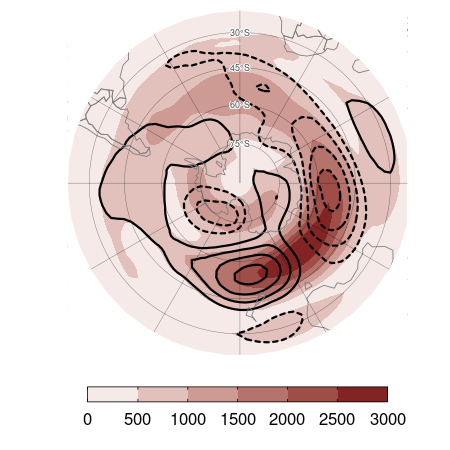
\includegraphics{figures/15-onda3/envolvente-ejemplo-1} 

}

\caption{Anomalías zonales de altura geopotencial en 500 hPa en septiembre de 1989 (contornos, líneas sólidas indican valores positivos y líneas punteadas indican valores negativos) y envolvente de ondas zonales (sombreado).}\label{fig:envolvente-ejemplo}
\end{figure}



La Figura \ref{fig:envolvente-ejemplo} muestra un ejemplo de la envolvente de la altura geopotencial en 500 hPa en septiembre de 1989
Las anomalías zonales de altura geopotencial son intensas al sur de Australia y Nueva Zelanda.
La envolvente captura esa región.

\hypertarget{resultados}{%
\section{Resultados}\label{resultados}}

\begin{figure}

{\centering 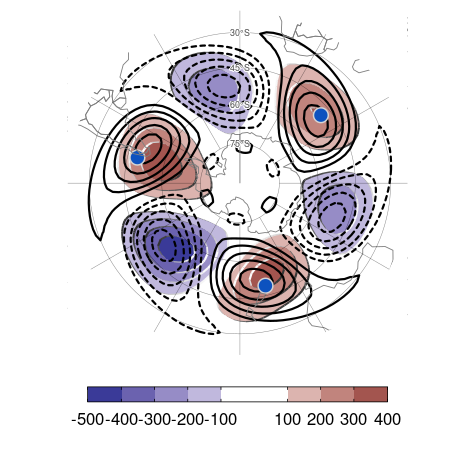
\includegraphics{figures/15-onda3/raphael-regr-1} 

}

\caption{Mapa de regresión entre R04 y la anomalía zonal de altura geopotencial en 500 hPa (sombreado) y onda 3 del campo medio de altura geopotencial en 500 hPa (contornos; valores positivos en línea llena y nagativos en línea punteada). En azul se indican la ubicación de los puntos usado para calcular R04.}\label{fig:raphael-regr}
\end{figure}



La Figura \ref{fig:raphael-regr} muestra las ubicaciones definidas por Raphael (2004) para calcular el índice y el mapa de regresión entre R04 y el campo de anomalías zonales de altura geopotencial en 500 hPa.
Se observa que representa una onda 3 relativamente pura con una amplitud ligeramente más alta en la región del Pacífico.
Sin embargo, se puede notar que los máximos al sur de Nueva Zelanda y sobre el pasaje de Drake se encuentran más al sur que los puntos usados de referencia.

La onda 3 descrita por R04 coincide bien con la onda 3 climatológica (contornos negros en la Fig \ref{fig:raphael-regr}).
Esto es por construcción, ya que al usar puntos fijos cercanos a estos máximos climatológicos, R04 busca medir la similitud del campo de anomalías zonales de altura geopotencial con la onda 3 climatológica.

\begin{figure}

{\centering 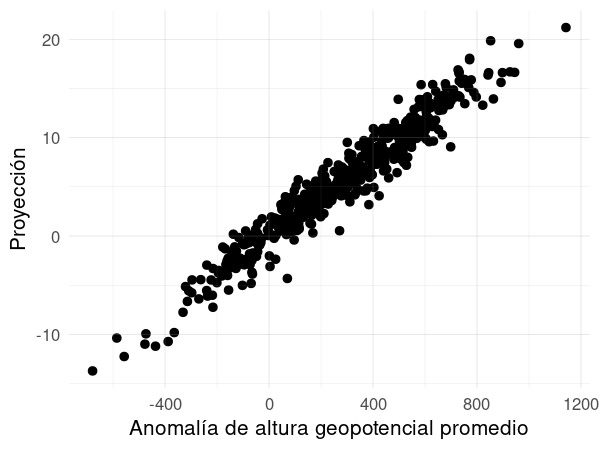
\includegraphics{figures/15-onda3/pseudo-raphael-1} 

}

\caption{Relación entre la anomalía zonal de altura geopotencial en los tres puntos utilizados por R04 y la amplitud de la proyección de la geopotencial en 50ºS, 500 hPa con la onda 3 climatológica.}\label{fig:pseudo-raphael}
\end{figure}



La Figura \ref{fig:pseudo-raphael} muestra la relación entre la proyección de la altura geopotencial en 50ºS con la onda 3 climatológica en esa latitud y la anomalía zonal de altura geopotencial promediada en las tres ubicaciones de R04 --esto no es exactamente el índice R04 ya que éste se calcula a partir de un promedio móvil de 3 meses y una estandarización previa al promediado.
Ambas series son casi idénticas, con una correlación de 0.97 (CI: 0.96 -- 0.97).
Esto ilustra que el índice R04 no es un índice de la amplitud de al onda 3, sino un índice de cuánto se parecen la altura geopotencial en 50ºS a la onda 3 media en 50ºS.

Si bien la Figura \ref{fig:raphael-regr} muestra que R04 está asociado con una onda 3 relativamente pura, no es sorprendente que un índice basado en el promedio de 3 puntos esté altamente correlacionado con regiones cercanas a esos puntos.
Esto no demuestra que éste sea un patrón físicamente coherente.

Para investigar la consistencia física de R04 se puede analizar la covariabilidad entre las tres regiones utilizadas para calcularlo.

\begin{table}

\caption{\label{tab:raphael-correlation}Correlación entre la anomalía zonal de geopotential en los tres puntos considerados por Raphael.}
\centering
\begin{tabular}[t]{cccc}
\toprule
 & 50°E & 165°E & 75°O\\
\midrule
50°E & 1.00 & 0.15 & -0.13\\
165°E & 0.15 & 1.00 & 0.04\\
75°O & -0.13 & 0.04 & 1.00\\
\bottomrule
\end{tabular}
\end{table}

La Tabla \ref{tab:raphael-correlation} muestra la matriz de correlación entre la anomalía zonal de altura geopotencial en las ubicaciones utilizada para calcular el índice R04, indicadas por su longitud.
Las correlaciones son muy cercanas a cero, e incluso la correlación entre el punto de 75ºO y 50ºE es negativa.
Esto indica que los puntos no son covariantes y sugiere que no representan un patrón coherente.

\begin{figure}

{\centering 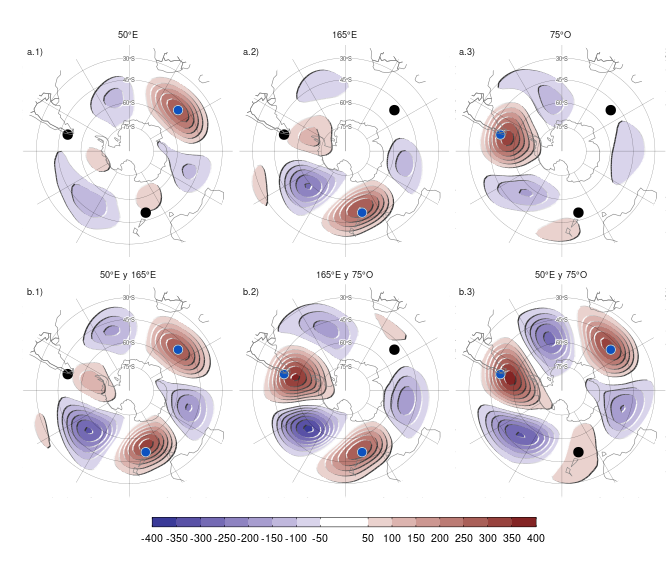
\includegraphics{figures/15-onda3/cor-puntos-1} 

}

\caption{Regresión entre la anomalía zonal de altura geopotencial en 500 hPa e índices R04 usando combinaciones de 1 y 2 puntos. En cada panel, los puntos azules son los puntos usados para calcular el índice y los negros, los excluidos.}\label{fig:cor-puntos}
\end{figure}



La Figura \ref{fig:cor-puntos} muestra los campos de regresión de anomalía zonal de altura geopotencial con índices pseudo-R04 computados utilizando sólo un punto (fila a) o promedios de dos puntos (fila b).
No hay un patrón coherente asociado a los puntos individuales.
Las combinaciones de dos puntos se asocian a anomalías positivas en los dos puntos relevantes y negativas entre los mismos --esperable ya que se trata de anomalías zonales-- pero, crucialmente, no hay una asociación positiva con el tercer punto no incluido en el índice.

\begin{figure}

{\centering \subfloat[Meses con mayor valor de R04\label{fig:raphael-top8-1}]{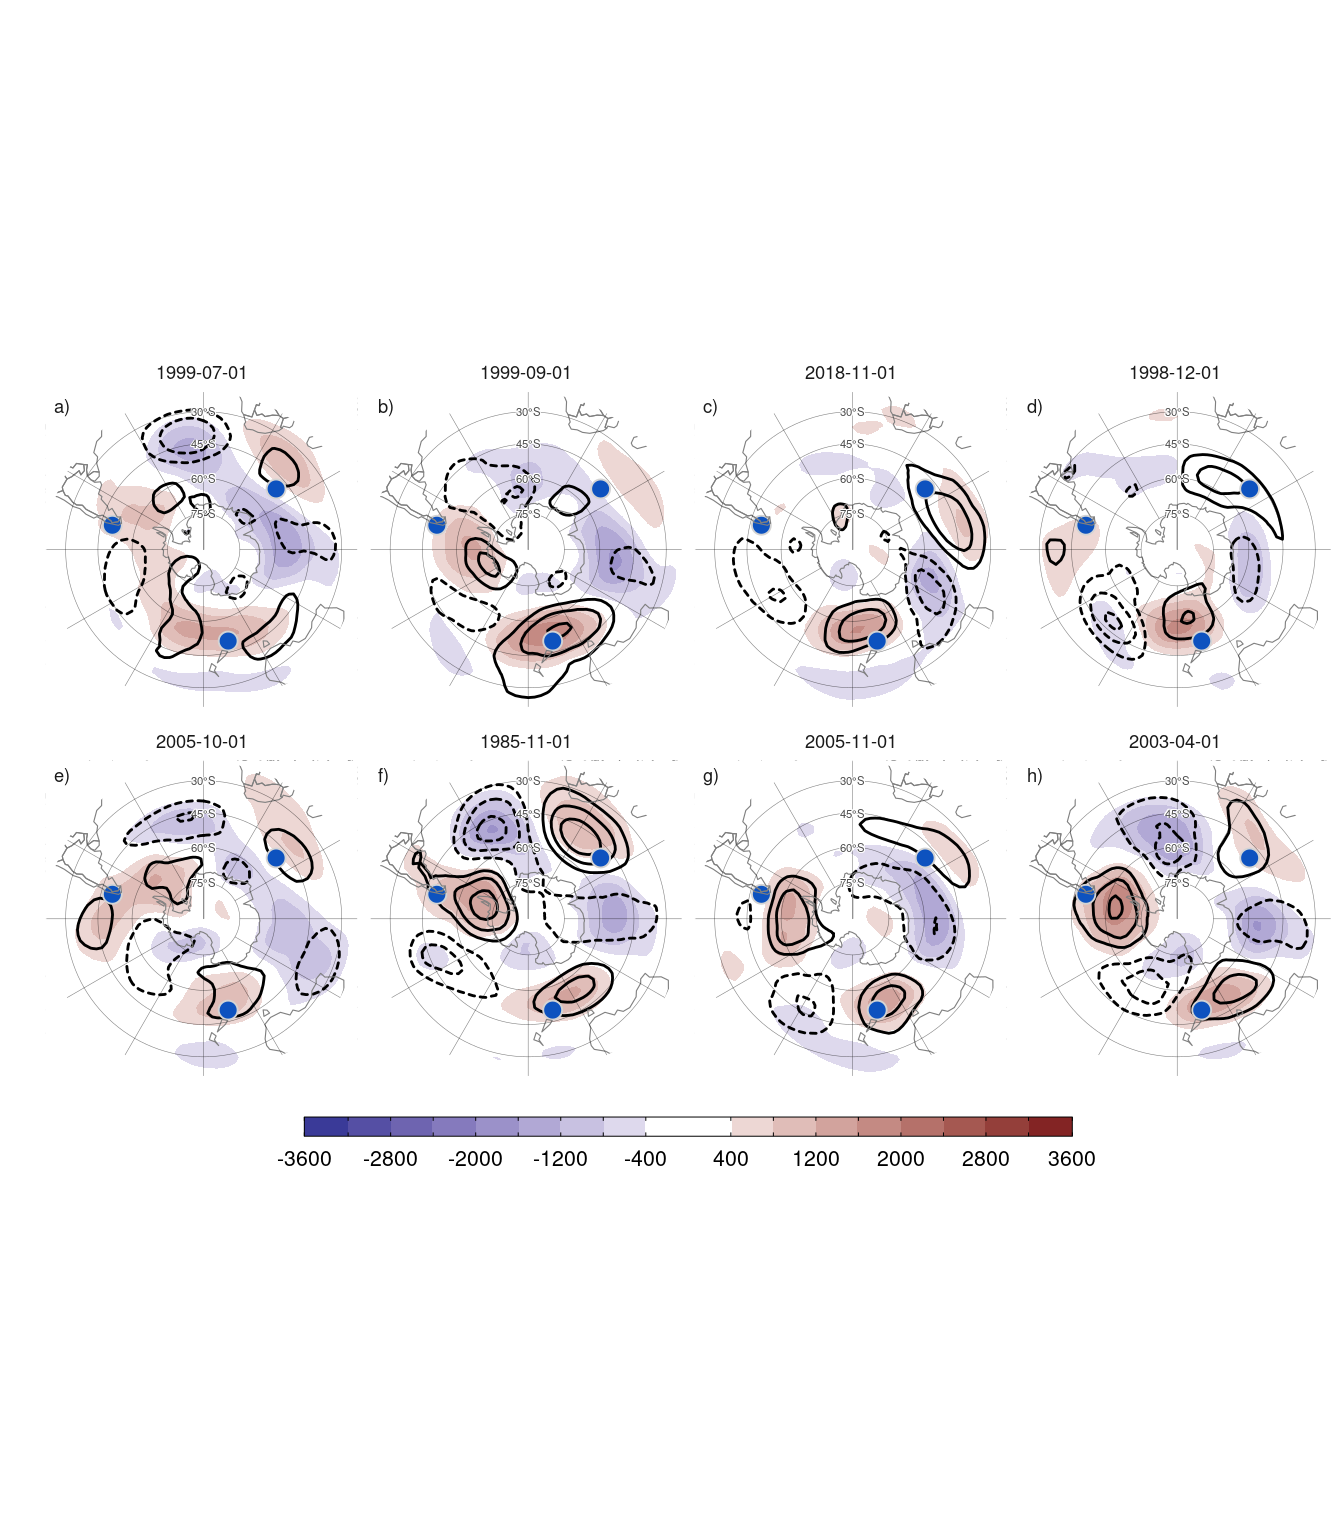
\includegraphics{figures/15-onda3/raphael-top8-1} }\newline\subfloat[Meses con menor valor de R04\label{fig:raphael-top8-2}]{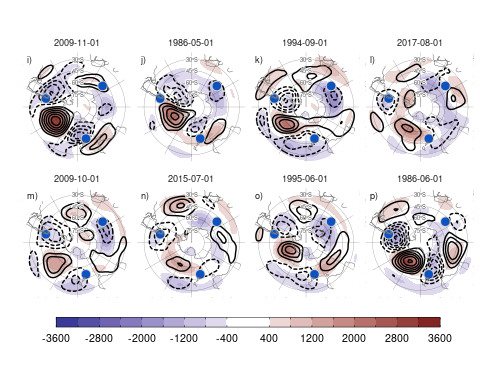
\includegraphics{figures/15-onda3/raphael-top8-2} }

}

\caption{Anomalía zonal de altura geopotencial (sombreado) y anomalía mensual de la anomalía zonal de altura geopotencial (contornos, valores positivos en línea sólida y valores negativos en línea punteada) en 500 hPa para los 8 meses con mayor y menor valor del índice R04. Los puntos azules indican las ubicaciones usadas en el índice R04.}\label{fig:raphael-top8}
\end{figure}



Finalmente, las Figuras \ref{fig:raphael-top8-1} y \ref{fig:raphael-top8-2} muestran la anomalía zonal y la anomalía mensual de la anomalía zonal de altura geopotencial en los los 8 meses con mayor y menor valor del índice, respectivamente.
En pocos casos se observa un patrón de onda 3 bien marcado; por ejemplo, en abril de 2003 y noviembre de 1985 (paneles f y g) se observan tres zonas de anomalías positivas cercanas a las ubicaciones utilizadas para calcular R04 y tres zonas de anomalías negativas entre las mismas.
En octubre de 2009 (panel o) se observa lo contrario.
En casos para los cuales el índice es positivo no hay siquiera anomalías positivas en los tres puntos, como en noviembre de 2018 (panel b) diciembre de 1998 (panel e).
En los casos negativos, parece haber un patrón de onda tipo PSA algo más definido, sin embargo, tampoco en estos casos hay buena consistencia entre los puntos.

De este análisis se desprende que el índice propuesto por Raphael (2004) no parece representar un fenómeno distintivo de onda 3.

Otra forma de medir la onda 3 es computando la amplitud de fourier de esta onda a lo largo de un circulo de latitud.
El modelo de fourier también asume que la onda 3 tiene una amplitud constante a lo largo de todo el círculo de latitud y que no presenta propagación meridional.
Esta medida no mide exactamente lo mismo que R04, ya que es sensible a la amplitud de la onda 3 sin importar dónde este localizada.
Esto puede observarse en la Figura \ref{fig:fase-histogram}, donde se observa que la localización de la onda 3 varía considerablemente.

\begin{figure}

{\centering 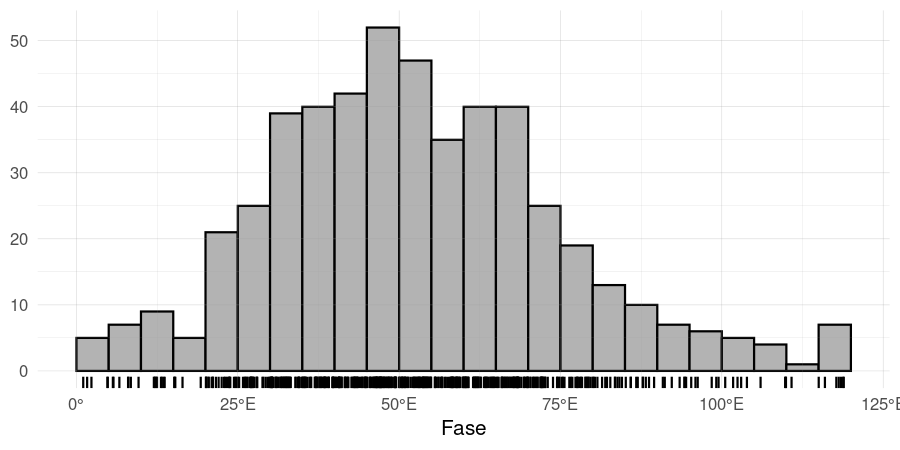
\includegraphics{figures/15-onda3/fase-histogram-1} 

}

\caption{Histograma de la fase de la onda 3 de altura geopotencial en 500 hPa.}\label{fig:fase-histogram}
\end{figure}



Por otro lado, la onda 3 de la altura geopotencial no es idéntica a la onda 3 de las anomalías mensuales de altura geopotencial.
Dado que la variable relevante para estudiar la variabilidad, los impactos, los forzantes y las tendencias son las anomalías con respecto a la media, desde ahora vamos a analizar las anomalías mensuales.

\begin{figure}

{\centering 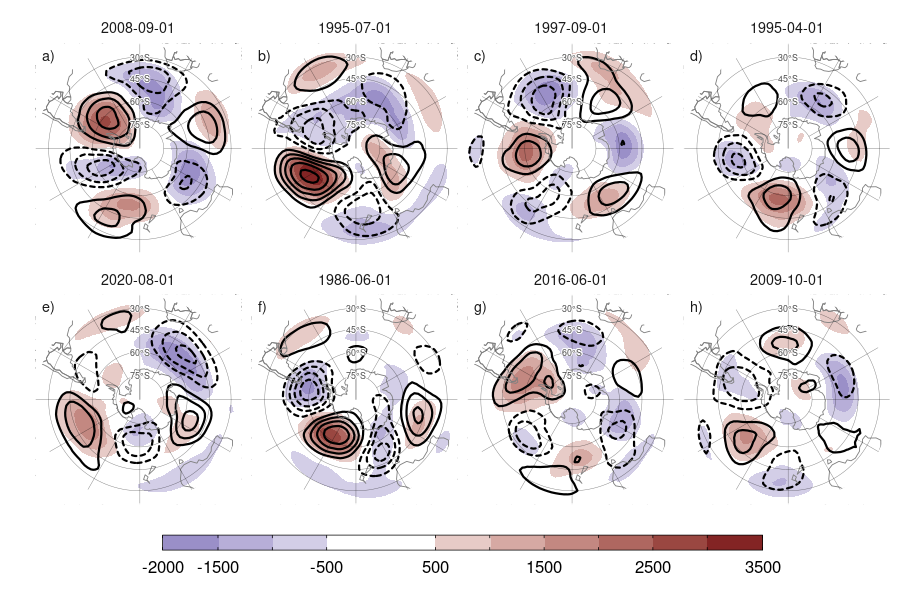
\includegraphics{figures/15-onda3/zw3-top8-1} 

}

\caption{Igual que la Figura \ref{fig:raphael-top8}, pero para los 8 meses con mayor amplitud de la onda 3 de la anomalía mensual de altura geopotencial en 500 hPa.}\label{fig:zw3-top8}
\end{figure}



La Figura \ref{fig:zw3-top8} es equivalente a la Figura \ref{fig:raphael-top8} pero para los 8 meses con mayor amplitud de la onda 3 de anomalía mensual de altura geopotencial en 500 hPa.
Se observa que una amplitud alta se asocia a una onda 3 relativamente clara, pero que su amplitud no es constante en todo el hemisferio.
Por ejemplo, la mayor amplitud de la onda 3 se observa en septiembre de 2008 (panel a).
Las anomalías zonales tienen mayor intensidad y se encuentran más al sur en la zona del pacífico y al este de Sudamérica que en el Índico y al sur de Australia.

\begin{figure}

{\centering 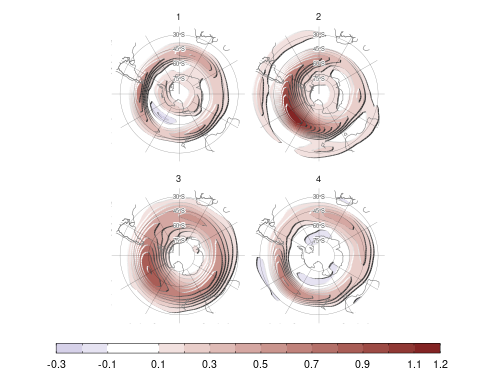
\includegraphics{figures/15-onda3/envelope-regr-1} 

}

\caption{Regresión entre la amplitud de las ondas 1 a 4 y la envolvente de todas las ondas zonales de las anomalías de altura geopotencial.}\label{fig:envelope-regr}
\end{figure}



Esta diferencia longitudinal en la amplitud de las ondas puede capturarse a partir de la envolvente de las ondas.
La Figura \ref{fig:envelope-regr} muestra la regresión entre la amplitud de las ondas 1 a 4 y la envolvente de todas las ondas zonales de las anomalías de altura geopotencial.
Se observa que la amplitud de la onda 1 se asocia a mayor actividad de onda en una banda aproximadamente zonalmente simétrica, indicando que la onda 1 contribuye con las anomalías zonales aproximadamente en todas las longitudes.
Las ondas 2 y 3, en cambio, contribuyen a las anomalías mensuales de altura geopotencial principalmente en el Pacífico sur.
Esto es consistente con lo observado en casos particulares en la Figura \ref{fig:zw3-top8} y sugiere que la onda 3 es más localizada que un modelo sinusoidal puro.

\hypertarget{conclusiones}{%
\section{Conclusiones}\label{conclusiones}}

De este análisis concluimos que ni el modelo de Raphael (2004) ni el modelo de Fourier son adecuados para estudiar la onda 3 en el hemisferio sur.
Es necesario un modelo que permita detectar cambios en la fase, modulación zonal de la amplitud y propagación meridional.
En el próximo capítulo presentamos un índice basado en Funciones Empíricas Ortogonales Complejas (cEOF) que resuelve estos problemas.

\hypertarget{ceofs}{%
\chapter{Modos de variabilidad de la circulación zonalmente asimétrica en primavera}\label{ceofs}}

\hypertarget{introducciuxf3n}{%
\section{Introducción}\label{introducciuxf3n}}

Dadas las deficiencias de los índices analizados previamente, es necesaria una metodología alternativa para caracterizar la circulación zonalmente asimétrica.
Proponemos el uso de Funciones Ortogonales Empíricas Complejas (cEOF) (Horel 1984), ya que éstas permiten caracterizar modos de variabilidad con amplitud y fase variable en el tiempo y con una estructura espacial más compleja que ondas sinusoidales constantes por cada círculo de latitud.

En base a exploraciones preliminares, en este capítulo nos restringimos al trimestre septiembre-octubre-noviembre (SON) ya durante esta estación las teleconexiones sobre Sudamérica son más intensas (Cazes-Boezio, Robertson y Mechoso 2003).
Muchas de las características de los cEOF son similares en los otros trimestres a excepción del trimestre diciembre-enero-febrero, el cual tiene características distintas.

Analizamos el nivel de 200 hPa dado que es un nivel cercano al máximo de la amplitud de la onda 3 (Campitelli 2018).
Dada la importancia de la variabilidad estratosférica en modular la propagación de las ondas, también incluimos el nivel de 50 hPa.

\hypertarget{muxe9todos-2}{%
\section{Métodos}\label{muxe9todos-2}}

\hypertarget{ceof-metodo}{%
\subsection{Funciones ortogonales complejas (cEOF)}\label{ceof-metodo}}



\begin{figure}

{\centering 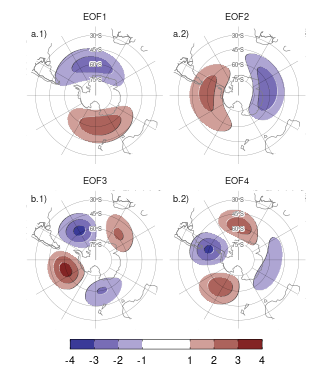
\includegraphics{figures/20-ceofs/eof-naive-1} 

}

\caption{Patrones espaciales de los primeros EOFs de las anomalías zonales de altura geopotencial en 50 hPa al sur de 20ºS. Para el período 1979--2020 (unidades arbitrarias).}\label{fig:eof-naive}
\end{figure}

Una de las metodologías más extendidas para analizar la variabilidad espacio-temporal de una variable es la de Funciones Ortogonales Empíricas (EOF) o componentes principales.
La Figura \ref{fig:eof-naive} muestra las cuatro priemras EOFs de las anomalías zonales de altura geopotencial de SON en 50 hPa al sur de 20º S.
Se puede observar que los dos primeros EOFs representan un único patrón de una onda zonal 1 no estacionario (es decir, un patrón con características espaciales similares donde la localización de los máximos varía).
Dado que los EOFs estándar sólo pueden representar patrones estacionarios (Horel 1984), ésta onda aparece como un par de EOFs girados en 1/4 de longitud de onda (90º en el espacio de frecuencias).
La amplitud de esta onda 1 podría medirse como \(\sqrt{\mathrm{PC1}^2 + \mathrm{PC2}^2}\) y su fase como \(\tan^{-1} \left ( \frac{\mathrm{PC2}}{\mathrm{PC1}} \right )\) (donde \(\mathrm{PC1}\) y \(\mathrm{PC2}\) son las series temporales asociadas a cada EOF).
Lo mismo sucede con el siguiente par de EOFs (EOF3 y EOF4), los cuales representan un mismo patrón con una escala espacial menor.
Pero esto se fundamenta en la inspección visual cualitativa de estos patrones espaciales y sólo funciona correctamente si ambas fases aparecen claramente divididas en estos dos EOFs, lo cual no está garantizado por construcción.

Una mejor alternativa para representar ondas que varían en su fase es utilizando el análisis de Funciones Ortogonales Empíricas Complejas (cEOF, por sus siglas en inglés) (Horel 1984).
Cada cEOF es un conjunto de patrones espaciales y series temporales con números complejos.
Las componentes real e imaginaria del patrón espacial complejo son la representación de dos patrones espaciales que están desplazados 1/4 de longitud de onda, similar a EOF1 y EOF2 en la Figura \ref{fig:eof-naive}.
En este trabajo nor referiremos a cada fase de un cEOF como la fase de 0º y la fase de 90º.
El campo real reconstruido por cada cEOF es la combinación lineal de los dos campos espaciales ponderados por sus respectivas series temporales.
Esto es análogo a cómo cualquier onda sinusoidal de fase y amplitud arbitraria puede construirse mediante la suma de un seno y un coseno de diferente amplitud pero fase fija.
Esto significa que los cEOF representan de forma natural patrones ondulatorios que cambian tanto su ubicación como su amplitud.

Por ejemplo, cuando las anomalías zonales de altura geopotencial se parecen mucho a la fase 0º del cEOF, entonces la serie temporal de esta fase es positiva y la serie temporal de la fase 90º es cercana a cero.
Del mismo modo, cuando las anomalías zonales de altura geopotencial se parecen a la fase 90º, la serie temporal de ésta es positiva y la serie temporal de la fase de 0º es cercana a cero.
Cuando las anomalías zonales de altura geopotencial tiene los máximos en una localización intermedia, entonces ambas series temporales tienen valores distintos a cero.

El signo de los EOF tradicionales no está determinado unívocamente, por lo que se puede multiplicar cada EOF por -1 (tanto su serie temporal como su patrón espacial) y obtener una descripción igualmente válida.
Este cambio de signo en los números reales corresponde a una rotación en el plano complejo de 0 o \(\pi\).
De forma similar, los cEOF no tienen un argumento (entendiendo los números complejos como una magnitud y un argumento) definido, por lo que pueden rotarse en el plano complejo con cualquier ángulo entre 0 y \(2\pi\) (Horel 1984); esto es una multiplicación por \(\cos(\alpha) + i\sin(\alpha)\) con \(\alpha\) cualquier número real entre 0 y \(2\pi\).

El procedimiento para calcular los cEOF es similar al de computar los EOF con la única diferencia de que los datos de entrada primero se convierten en su señal analítica.
Ésta es un número complejo cuya parte real es la serie original y cuya parte imaginaria son los datos originales desplazados 90º en cada frecuencia espectral, es decir, su transformada de Hilbert.
La transformada de Hilbert suele entenderse en términos de señal variable en el tiempo, pero las ondas zonales son estructuras con forma de onda en el sentido zonal.
Por esto calculamos la transformada de Hilbert de las anomalías zonales de altura geopotencial variable en cada longitud; es decir, calculada para cada nivel, tiempo y latitud.
Dado que cada círculo de latitud es un dominio periódico, este procedimiento no sufre efectos de borde.



\begin{figure}

{\centering 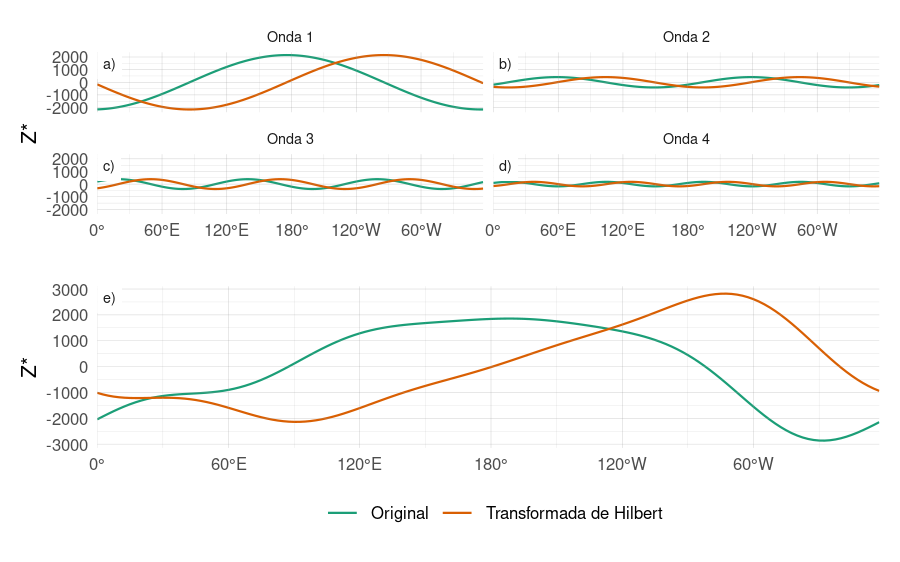
\includegraphics{figures/20-ceofs/hilbert-ejemplo-1} 

}

\caption{Ejemplo de cálculo de la función analítica de la señal de anomalías zonales de altura geopotencial. Los primeros cuatro paneles muestran las cuatro primeras ondas zonales y el último la señal completa. En verde se muestra la señal original y en naranja la transformada de Hilbert.}\label{fig:hilbert-ejemplo}
\end{figure}

La Figura \ref{fig:hilbert-ejemplo} ilustra la señal analítica con las anomalías zonales de geopotencial de SON en 1982 en 50hPa y 50ºS donde la línea verde es la señal original y la línea naranja es la transformada de Hilbert.
En los primeros paneles la señal está dividida en las ondas zonales 1 a 4 donde se ve con claridad como la transformada de Hilbert es la misma señal pero desplazada 1/4 de longitud de onda.



\begin{table}

\caption{\label{tab:corr-ceof-splitted}(ref:cor r-ceof-splitted-cap)}
\centering
\begin{tabular}[t]{l>{}r>{}r>{}r}
\toprule
\multicolumn{1}{c}{} & \multicolumn{3}{c}{50 hPa} \\
\cmidrule(l{3pt}r{3pt}){2-4}
200 hPa & cEOF1 & cEOF2 & cEOF3\\
\midrule
cEOF1 & \textbf{0.29} & 0.01 & 0.03\\
cEOF2 & 0.00 & \textbf{0.59} & 0.02\\
cEOF3 & 0.00 & 0.00 & 0.01\\
\bottomrule
\end{tabular}
\end{table}

La Tabla \ref{tab:corr-ceof-splitted} muestra el coeficiente de determinación de la magnitud de las series temporales de los cEOF entre 50 y 200 hPa.
Existe un alto grado de correlación entre la magnitud de los respectivos cEOF1 y cEOF2 en cada nivel.
Los patrones espaciales de los cEOF de 50 hPa y 200 hPa también son similares (no se muestra).

Tanto la similitud del patrón espacial como la alta correlación temporal de los cEOF calculados a 50 hPa y 200 hPa sugieren que se trata, en gran medida, de modos de variabilidad conjunta.
Esto motiva la decisión de calcular los cEOF en ambos niveles conjuntamente.
El resultado es que cada cEOF tiene una componente espacial que depende de la longitud, la latitud y el nivel, y una componente temporal que sólo depende del tiempo.
Dada las diferencias de magnitud entre la variabilidad de la altura geopotencial en 50 hPa y 200 hPa, se estandarizaron las variables de cada nivel por su desvío estándar.

Como se mencionó anteriormente, el argumento de los cEOF no está determinado unívocamente y se le puede sumar una constante real arbitraria.
Para facilitar la interpretación y permitir la reproducibilidad, definimos el argumento de cada cEOF de modo que alguna de las dos fases esté alineada con alguna variable significativa de nuestro análisis.
Este procedimiento no crea correlaciones espurias, sólo toma una relación existente y la alinea con una fase específica.

Un análisis preliminar mostró que el cEOF1 está estrechamente relacionado con la onda zonal 1 de la Columna Total de Ozono (CTO) y el segundo cEOF está estrechamente relacionado con el ENSO.
Por lo tanto, elegimos el argumento del cEOF1 de forma que la serie temporal correspondiente al cEOF1 de 0º tenga la máxima correlación con la onda zonal 1 del CTO entre 75°S y 45°S.
Del mismo modo, elegimos el argumento del cEOF2 de modo que el coeficiente de determinación entre el ONI y el cEOF2 de 0º sea mínimo, lo que también casi maximiza la correlación con el cEOF2 de 90º.

En la Sección \ref{impactos} mostramos regresiones de precipitación y temperatura asociadas a fases intermedias entre 0º y 90º.
Para esos gráficos, giramos los cEOF en 1/4 de longitud de onda multiplicando las series temporales complejas por \(\cos(\pi/4) + i\sin(\pi/4)\) y calculando la regresión sobre esas series temporales rotadas.

Si bien los cEOFs se calcularon para el período 1979--2020, extendimos las series temporales complejas hasta el periodo 1950--1978 proyectando las anomalías zonales mensuales de altura geopotencial normalizadas por nivel al sur de 20ºS sobre los patrones espaciales correspondientes.

\hypertarget{resultados-1}{%
\section{Resultados}\label{resultados-1}}

\hypertarget{caracterizaciuxf3n-espacio-temporal-de-los-modos}{%
\subsection{Caracterización espacio-temporal de los modos}\label{caracterizaciuxf3n-espacio-temporal-de-los-modos}}



\begin{figure}

{\centering 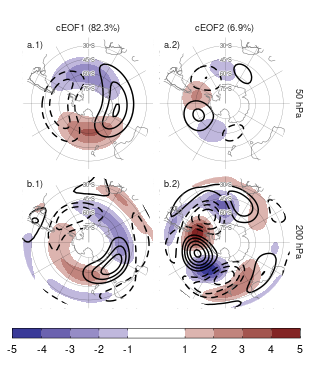
\includegraphics{figures/20-ceofs/ceofs-1-1} 

}

\caption{Patrones espaciales de los dos primeros cEOF de las anomalías zonales de altura geopotencial de SON en 50 y 200 hPa para el período 1979--2020. El sombreado corresponde a la fase 0º y los contornos, a la fase 90º. La proporción de varianza explicada por cada modo con respecto a la media zonal está indicada entre paréntesis. Las unidades son arbitrarias.}\label{fig:ceofs-1}
\end{figure}



\begin{figure}

{\centering 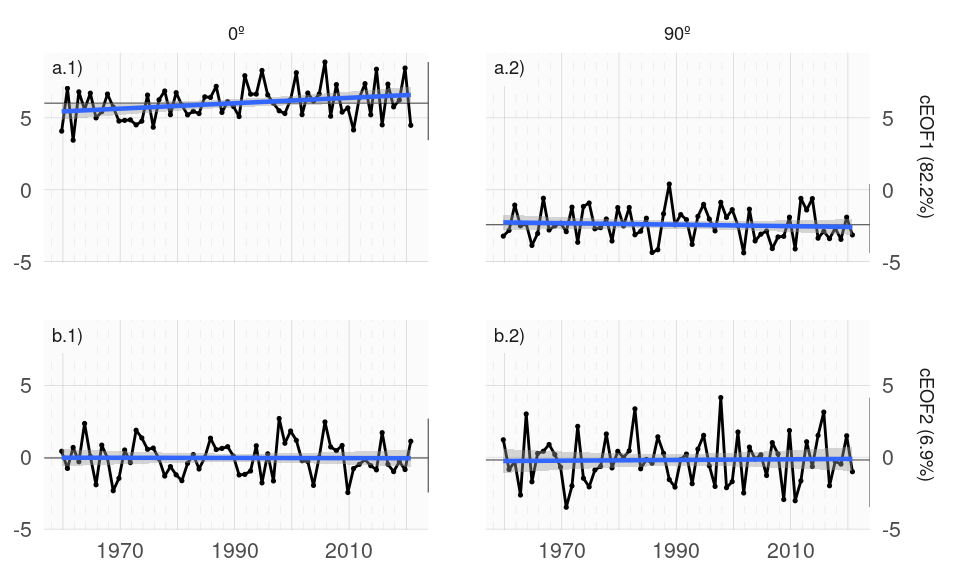
\includegraphics{figures/20-ceofs/extended-series-1} 

}

\caption{Series temporales de los dos primeros cEOF de las anomalías zonales de altura geopotencial de SON en 50 y 200 hPa para el período 1979--2020. El cEOF1 (fila a) y cEOF2 (fila b) separados en la fase 0º (columna 1) y la fase 90º (columna 2). Las líneas oscuras muestran la tendencia lineal de todo el período. Las líneas negras horizontales y verticales muestran el valor medio y el rango de cada serie, respectivamente. La proporción de varianza explicada por cada modo con respecto a la media zonal está indicada entre paréntesis. Las unidades son arbitrarias.}\label{fig:extended-series}
\end{figure}

Las Figuras \ref{fig:ceofs-1} y \ref{fig:extended-series} muestran las partes espacial y temporal de los dos primeros cEOFs de las anomalías zonales de la altura geopotencial en 50 hPa y 200 hPa, calculados conjuntamente en ambos niveles.
El primer modo (cEOF1) explica el 82\% de la varianza de las anomalías zonales, mientras que el segundo modo (cEOF2) explica una fracción menor (7\%).
En los patrones espaciales (Fig. \ref{fig:ceofs-1}), las fases de 0º y 90º están en cuadratura por construcción, de modo que cada cEOF describe un único patrón ondulatorio cuya amplitud y fase está controlada por la magnitud y fase de su serie temporal.

El cEOF1 (Fig. \ref{fig:ceofs-1} columna 1) es un patrón de onda 1 con amplitud máxima en latitudes altas.
En 50 hPa la fase de 0º del cEOF1tiene el máximo de la onda 1 en 150ºE y en 200 hPal máximo se sitúa en torno a 175ºE indicando un desplazamiento hacia el oeste con la altura.
El cEOF2 (Fig. \ref{fig:eof-naive} columna 2) muestra también una estructura de onda zonal con amplitud máxima en latitudes altas, pero con escalas espaciales más cortas.
En particular, la estructura dominante a ambos niveles es una onda 3 pero con mayor amplitud en el sector del océano Pacífico.
No hay cambio de fase aparente con la altura, pero la amplitud del patrón se reduce considerablemente en la estratosfera, lo que es coherente con el hecho de que el cEOF2 calculado por separado para 200 hPa explica un porcentaje mayor de la varianza que el cEOF2 calculado por separado para 50 hPa (11\% vs.~3\%, respectivamente).
Esto sugiere que este modo barotrópico representa principalmente la variabilidad troposférica.

No existe una correlación significativa entre las series temporales de los cEOFs.
Ambos cEOF muestran variabilidad interanual pero no muestran evidencia de variabilidad decadal (Fig. \ref{fig:extended-series}).
Debido a que los campos que entran en el algoritmo de cEOF son anomalías con respecto a la media zonal en lugar de la media temporal, las series temporales de los cEOF tienen media temporal no nula.
Sin embargo, la media temporal de cEOF2 es casi cero, lo que indica que sólo cEOF1 incluye variabilidad que se proyecta significativamente sobre el campo anómalo zonal medio.
Esto es coherente con el hecho de que el campo medio zonalmente anómalo de la altura geopotencial es muy similar al cEOF1 (\(r^2\) = 98\%) y no similar al cEOF2 (\(r^2\) = 0\%).

Es evidente una tendencia positiva significativa en la fase de 0º del cEOF1 (Fig. \ref{fig:extended-series}a.1, p-valor = 0.023), mientras que no hay tendencia significativa en ninguna de las fases de cEOF2.
La tendencia positiva de la fase de 0º del cEOF1 se traduce en una tendencia positiva en la magnitud del cEOF1, pero no en un cambio sistemático en la fase (no se muestra).
Este cambio a largo plazo indica un aumento de la magnitud de la onda zonal 1 de latitudes altas.

\hypertarget{mapas-de-regresiuxf3n-con-los-modos-ceof}{%
\subsection{Mapas de regresión con los modos cEOF}\label{mapas-de-regresiuxf3n-con-los-modos-ceof}}

\hypertarget{geopotencial}{%
\subsubsection{Geopotencial}\label{geopotencial}}

En la sección anterior mostramos los patrones espaciales de los cEOF obtenidos a partir de las anomalías zonales de altura geopotencial.
En esta sección calculamos campos de regresión de las series temporales de los cEOF con las anomalías temporales de altura geopotencial para describir la influencia de los cEOF en las anomalías temporales.



\begin{figure}

{\centering 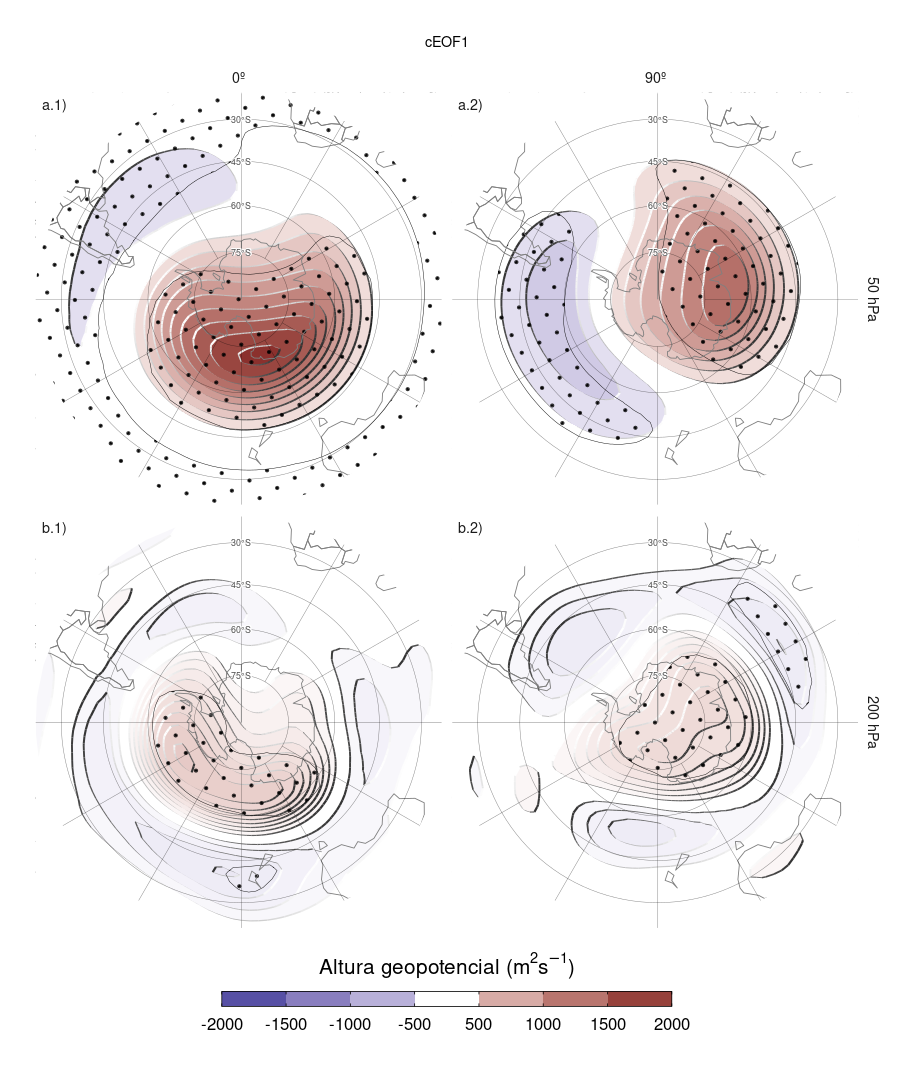
\includegraphics{figures/20-ceofs/eof1-regr-gh-1} 

}

\caption{Regresión de anomalías de temperatura geopotencial en SON (\(m^2s^{-1}\)) con la fase de 0º (columna 1) y de 90º (columna 2) del cEOF1 en 50 hPa (fila a) y 200 hPa (fila b) para el período 1979--2020. Estos coeficientes fueron obtenidos a partir de una regresión múltiple incluyendo ambas fases. Áreas con puntos marcan regiones donde el p-valor es menor que 0.01 ajustado por FDR.}\label{fig:eof1-regr-gh}
\end{figure}

La Figura \ref{fig:eof1-regr-gh} muestra los mapas de regresión de anomalías de altura geopotencial en SON con respecto al cEOF1.
En 50 hPa (Fig. \ref{fig:eof1-regr-gh} fila a), la fase de 0º del cEOF1 está asociada a un centro de anomalías positivas sobre la Antártida con su centro sobre el Mar de Ross.
Por otro lado, el centro de anomalías positivas asociado a la fase de 90º está corrido hacia Antártida Oriental y tiene un patrón de onda 1 más evidente.

En 200 hPa (Fig. \ref{fig:eof1-regr-gh} fila b) la fase de 0º del cEOF1 muestra un único centro de anomalías positivas que abarca la Antártida Occidental rodeado de anomalías opuestas en latitudes más bajas, con su centro desplazado ligeramente hacia el este en comparación con las anomalías de niveles superiores.
La fase de 90º muestra un patrón mucho más simétrico zonalmente que se asemeja al patrón de anomalías características de la fase negativa del SAM (Fogt y Marshall 2020).
En ambas fases las anomalías negativas en latitudes bajas son débiles y no son estadísticamente significativas

Por lo tanto, la magnitud y la fase del cEOF1 están asociadas a la magnitud y la fase de una onda zonal principalmente en la estratosfera.



\begin{figure}

{\centering 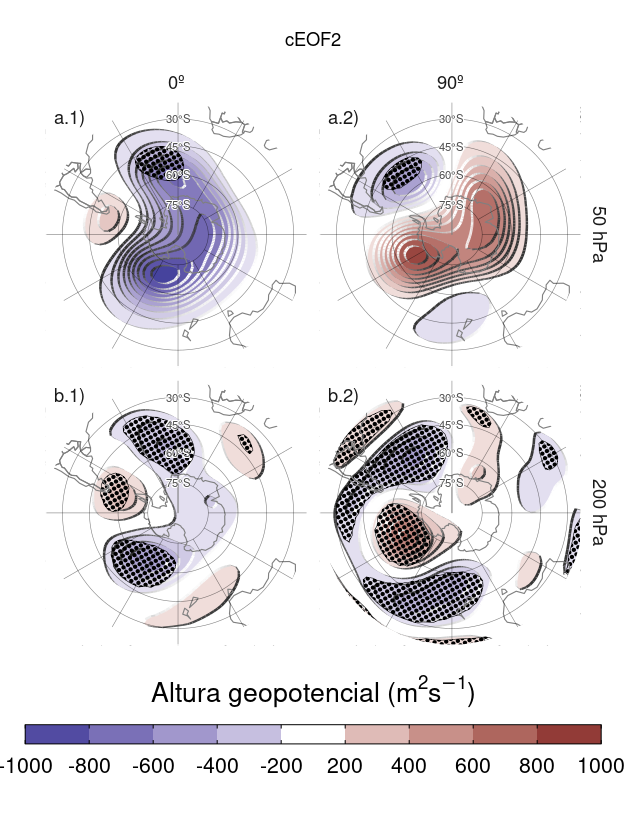
\includegraphics{figures/20-ceofs/eof2-regr-gh-1} 

}

\caption{Igual que la Figura \ref{fig:eof1-regr-gh} pero para el cEOF2.}\label{fig:eof2-regr-gh}
\end{figure}

La Figura \ref{fig:eof2-regr-gh} muestra los mapas de regresión de las anomalías de altura geopotencial con el cEOF2.
Tanto en 50 como en 200 hPa se observa un patrón de onda 3 similares a los de la Figura \ref{fig:ceofs-1} columna 2.
Las anomalías de regresión asociadas con la fase de 0º del cEOF2 están desfasadas 1/4 de longitud de onda con respecto a las asociadas con la fase de 90º.
Todos los campos tienen una onda zonal dominante 3 limitada al hemisferio occidental, sobre los océanos Pacífico y Atlántico.

En 50 hPa (Fig. \ref{fig:eof2-regr-gh} fila a) también se ve un monopolo sobre el polo con signo negativo asociado a la fase de 0º y signo positivo asociado a la fase de 90º.
Este monopolo podría indicar fortalecimiento del vórtice polar asociado a valores positivos de la fase de 0º del cEOF2 y debilitamiento asociado a valores negativos del la fase de 0º del cEOF2.
Sin embargo, estas anomalías no son estadísticamente significativas, indicando que su magnitud es baja en comparación a la variabilidad estratosférica y que esta característica no debe sobreinterpretarse.

En 200 hPa (Fig. \ref{fig:eof2-regr-gh} fila b) el tren de ondas es robusto ya que los centros son estadísticamente significativos, con anomalías insignificantes por fuera de este patrón.
La localización de las anomalías no varía en la vertical, lo cual indica que se trata de un modo barotrópico equivalente.

El cEOF2 representa entonces un tren de ondas barotrópico equivalente muy similar al de los Patrones PSA (Mo y Paegle 2001).
Comparando la localización de la anomalía positiva cerca de 90ºO en la columna 2 de la Figura \ref{fig:eof2-regr-gh} con las Figuras 1.a y b de Mo y Paegle (2001), el mapa de regresión de la fase de 0º podría identificarse con el PSA2, mientras que la fase 90º se asemeja al PSA1.
Por otro lado, ambos modos muestran relación con patrones anulares semejantes al SAM.
Estudiaremos la relación entre los cEOF y el PSA y con más detalle en el Capítulo \ref{sam-ceof}.

\hypertarget{temperatura-y-ozono}{%
\subsubsection{Temperatura y Ozono}\label{temperatura-y-ozono}}



\begin{figure}

{\centering 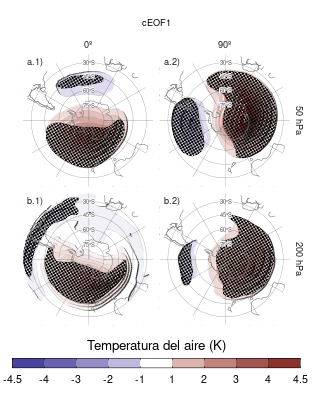
\includegraphics{figures/20-ceofs/eof1-regr-t-1} 

}

\caption{Igual que la Figura~\ref{fig:eof1-regr-gh} pero para la temperatura del aire (K).}\label{fig:eof1-regr-t}
\end{figure}



\begin{figure}

{\centering 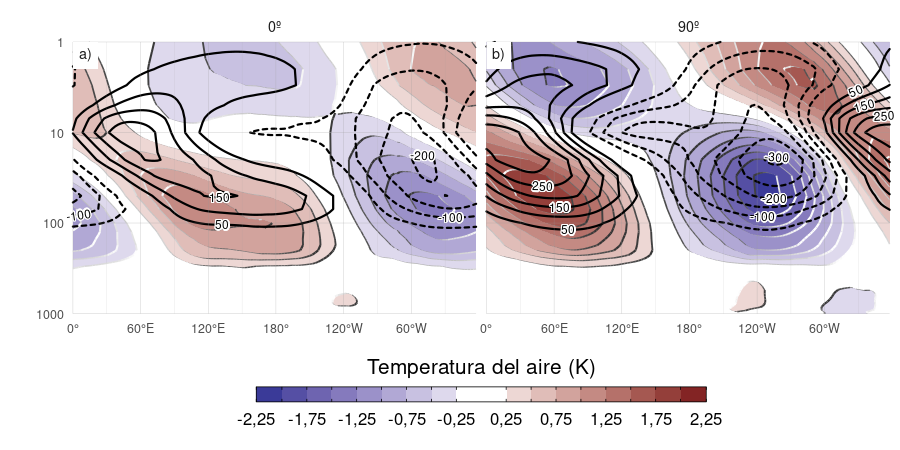
\includegraphics{figures/20-ceofs/t-vertical-1} 

}

\caption{Regresión de anomalías zonales de temperatura (sombrado, Kelvin) y razón de mezcla de ozono (contornos, valores negativos en línea punteada, etiquetas en partes por mil millón en masa) promediados entre 75°S y 45°S en SON con la fase de 0º (a) y de 90º (b) del cEOF1 para el período 1979--2020.}\label{fig:t-vertical}
\end{figure}

También evaluamos la señal de la variabilidad de los cEOF en la temperatura del aire.
La Figura \ref{fig:eof1-regr-t} muestra los mapas de regresión de las anomalías de la temperatura del aire en 50 hPa y 200 hPa con el cEOF1.
La distribución de los coeficientes de regresión de la temperatura en 50 hPa y en 200 hPa refleja los mapas de regresión de la altura geopotencial en 50 hPa (Fig. \ref{fig:eof1-regr-gh}).
En ambos niveles, la fase de 0º está asociada a anomalías positivas sobre el Polo Sur con su centro desplazado ligeramente hacia 150ºE (Fig. \ref{fig:eof1-regr-t} columna 1).
Por otro lado, los mapas de regresión con la fase de 90º muestran un patrón de onda 1 más claro con su máximo alrededor de los 60ºE.

La Figura \ref{fig:t-vertical} muestra la distribución vertical de los coeficientes de regresión del cEOF1 con las anomalías zonales de la temperatura del aire y de la razón de mezcla de ozono promediadas entre 75°S y 45°S.
Las anomalías zonales de temperatura asociadas al cEOF1 muestran un claro patrón de onda 1 tanto para la fase de 0º como para la de 90º en toda la atmósfera por encima de 250 hPa con una inversión de signo por encima de 10 hPa.
Como resultado del balance hidrostático, este es el nivel en el que la anomalía geopotencial tiene máxima amplitud (no mostrado).

Los valores máximos de la regresión con el ozono coinciden con los valores mínimos de temperatura por encima de 10 hPa y con los máximos por debajo de 10 hPa (Fig. \ref{fig:t-vertical}).
Por tanto, la onda zonal 1 de ozono está correlacionada negativamente con la onda zonal 1 de temperatura en la estratosfera superior, y positivamente en la estratosfera baja.
Este cambio de fase es observado en las anomalías de ozono forzadas por ondas planetarias que alcanzan la estratosfera.
En la estratosfera superior, dominada por procesos fotoquímicos, las temperaturas frías inhiben la destrucción de ozono, explicando el comportamiento opuesto para ambas variables, tal y como se dilucidó con modelos químicos dinámicos (Hartmann y Garcia 1979; Wirth 1993; Smith 1995).
Por otro lado, en la estratosfera baja, dominada por la advección, las anomalías de ozono están desfasadas 1/4 de longitud de onda con el transporte horizontal y vertical, que a su vez están desfasados 1/4 de longitud de onda con las anomalías de temperatura, resultando anomalías del mismo signo para la respuesta de ambas variables (Hartmann y Garcia 1979; Wirth 1993; Smith 1995).



\begin{figure}

{\centering 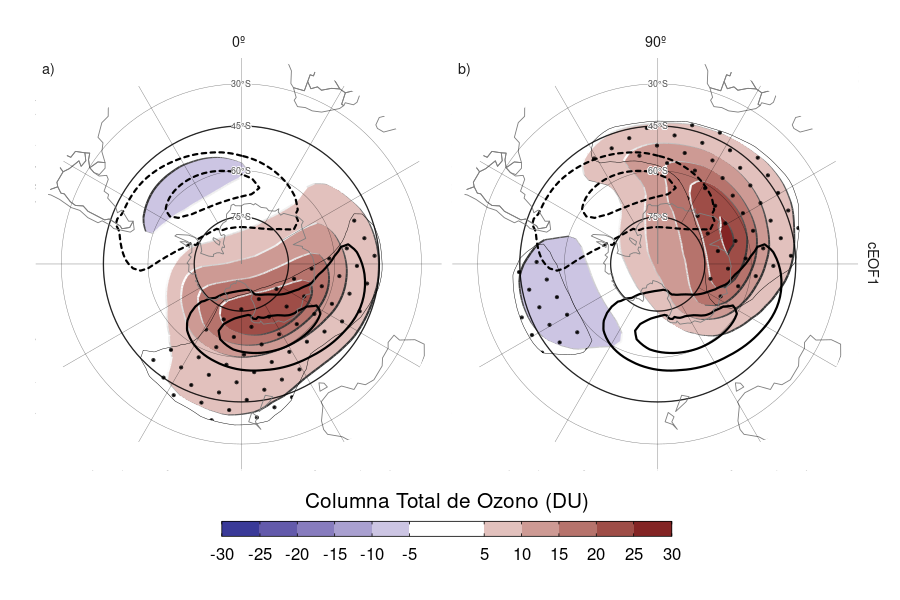
\includegraphics{figures/20-ceofs/o3-regr-1} 

}

\caption{Regresión de las anomalías de Columna Total de Ozono (CTO, sombreado, unidades Dobson) con la fase de 0º (a) y de 90º (b) del cEOF1 para el período 1979--2020. En contornos, la anomalía zonal media de de CTO (contornos negativos en líneas punteadas, unidades Dobson). Áreas con puntos marcan regiones donde el p-valor es menor que 0.01 ajustado por FDR.}\label{fig:o3-regr}
\end{figure}



Los mapas de regresión de las anomalías de CTO con el cEOF1 (Fig. \ref{fig:o3-regr}) muestran patrones de onda zonal 1 asociados a ambas fases del cEOF1.
La posición climatológica del mínimo de ozono durante la primavera (agujero de la capa de ozono) no está centrada sobre el Polo Sur, sino que está desplazada hacia el mar de Weddell (ej, Grytsai 2011); este desplazamiento se traduce en una onda 1 de la CTO.
Así, el campo de regresión de la fase de 0º del cEOF1 (Fig.~\ref{fig:o3-regr}a) coincide con la posición climatológica de esta onda 1 del agujero de ozono, mientras que el campo para la fase de 90º está defasado en 90º cEOF1.
La correlación temporal entre la amplitud de la onda 1 de CTO y la amplitud del cEOF1 es 0.79 (CI: 0.63 -- 0.88), mientras que la correlación entre sus fases es -0.85 (CI: -0.92 -- -0.74).
La correlación entre las dos ondas es -0.87 (CI: -0.93 -- -0.77).
En consecuencia, el cEOF1 está fuertemente relacionado con la variabilidad del ozono del hemisferio sur.

\hypertarget{fuentes-ceof}{%
\subsection{Fuentes de variabilidad tropicales}\label{fuentes-ceof}}



\begin{figure}

{\centering 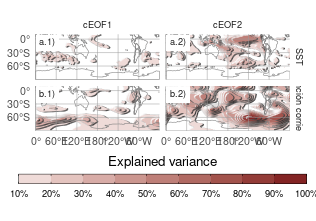
\includegraphics{figures/20-ceofs/psi-sst-explained-variance-1} 

}

\caption{Varianza de las anomalías de TSM (fila a) y de las anomalías zonales de función corriente (fila b) explicada por el cEOF1 (columna 1) el cEOF2 (columna 2).}\label{fig:psi-sst-explained-variance}
\end{figure}

Para evaluar si la variabilidad de los cEOF analizados está relacionada con fuentes de variabilidad tropicales calculamos la regresión de distintas fases de los cEOFs con las anomalías de TSM y con las anomalías zonales de función corriente a 200 hPa.
La Figura \ref{fig:psi-sst-explained-variance} muestra la varianza de cada variable explicada por cada cEOF.

El cEOF1 sólo explica una proporción importante de la varianza de la función corriente al sur de 60º, sugiriendo que no está asociado con la variabilidad tropical (Fig. \ref{fig:psi-sst-explained-variance} b.1).

El cEOF2, en cambio, explica una gran proporción de la variabilidad tropical tanto de las anomalías de TSM como de las de función corriente.
Este modo comparte más de un 50\% de la varianza con las TSM en el Pacífico central (sugiriendo el impacto del ENSO).
En cuanto a la función corriente, en el Pacífico explica más del 50\% de la varianza en la región del cambio de fecha y sobre Indonesia.
También explica gran parte de la varianza en al oeste y al este de la Península Antártica, llegando a más del 80\% sobre el mar de Amundsen.



\begin{figure}

{\centering 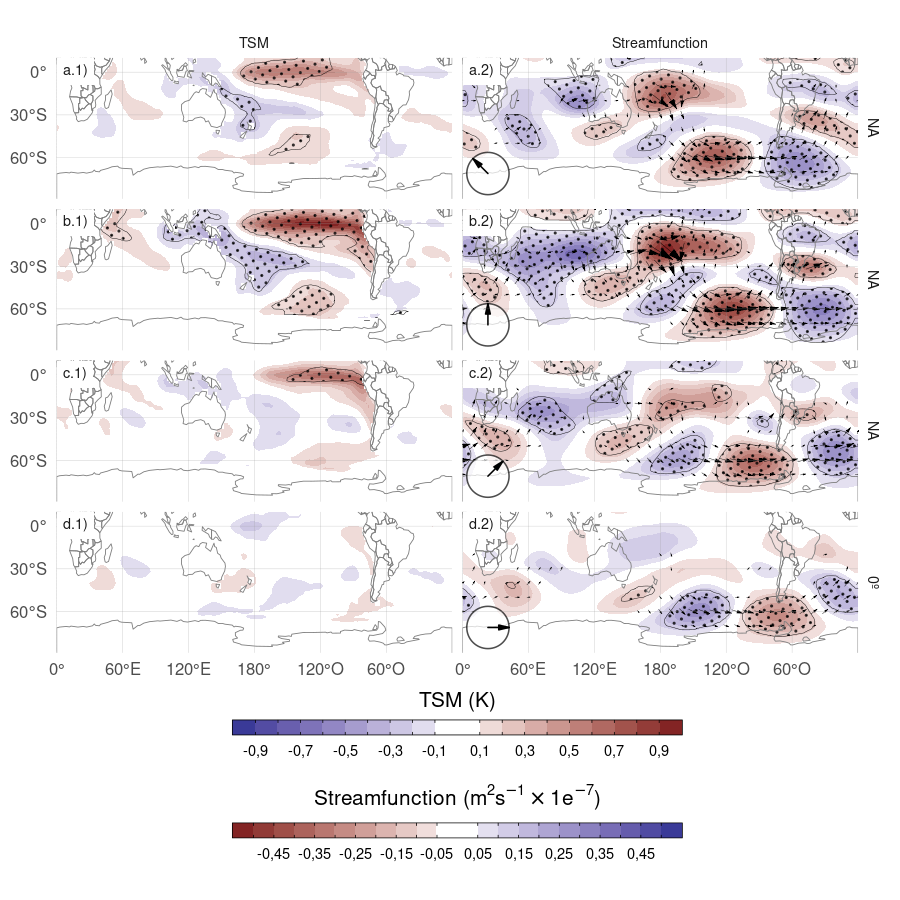
\includegraphics{figures/20-ceofs/sst-psi-2-1} 

}

\caption{Regresión de (columna 1) TSM (K) y (columna 2) anomalías zonales de función corriente (\(m^2/s\times10^-7\)) y sus vectores de acción de onda con diferentes fases del cEOF2 (indicado con la flecha) en el período 1979--2020. Áreas con puntos marcan regiones donde el p-valor es menor que 0.01 ajustado por FDR.}\label{fig:sst-psi-2}
\end{figure}

La Figura \ref{fig:sst-psi-2} muestra los mapas de regresión de las anomalías de la temperatura de la superficie del mar (TSM) y de la función de corriente a 200 hPa sobre los cEOF2 normalizados.
Además de los mapas de regresión para las fases de 0º y 90º, incluimos las regresiones correspondientes para dos direcciones intermedias (correspondientes a 45º y 135º).

La fase de 90º (fila b) está asociada a fuertes anomalías positivas de la TSM en el Pacífico central y oriental y a anomalías negativas en una zona que atraviesa el norte de Australia, Nueva Zelanda y la Zona de Convergencia del Pacífico Sur (SPCZ) (Fig. \ref{fig:sst-psi-2}.b1).
Este patrón es muy similar al patrón del ENSO positivo canónico (Bamston, Chelliah y Goldenberg 1997).
De hecho, existe una correlación significativa y muy alta entre el ONI y la serie temporal de la fase de 90º del cEOF2 (0.76 (CI: 0.6 -- 0.87)).
Además del patrón similar al ENSO del Pacífico, también hay anomalías positivas en el océano Índico occidental y valores negativos en el océano Índico oriental, lo que se asemeja a un dipolo del índico en su fase positiva (Saji et~al. 1999).
Consistentemente, la correlación entre la fase de 90º del cEOF2 y el DMI es 0.62 (CI: 0.38 -- 0.77).
Sin embargo, la correlación parcial es de 0.33 (p-valor = 0.037), indicando que el DMI explica poca varianza de la fase de 90º del cEOF2 por sí mismo.
Esto puede observarse en la Figura \ref{fig:euler}, donde se ilustra la partición de la varianza de la fase de 90º del cEOF2, el DMI y el ONI.
El DMI aporta, independientemente, sólo un 4.3\% de la varianza mientras que el ONI aporta un 23.9\% por sí mismo.

\begin{figure}

{\centering 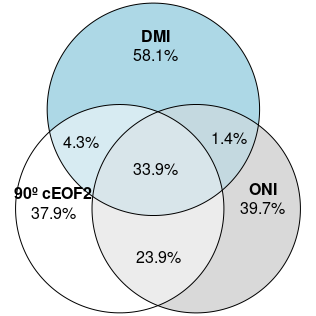
\includegraphics{figures/20-ceofs/euler-1} 

}

\caption{Diagrama de Euler mostrando la proporción de la varianza de cada serie (DMI, ONI y la fase de 90º del cEOF2) explicada por las demás (p.e. la región común entre DMI y ONI es la varianza del DMI explicada por el ONI y viceversa).}\label{fig:euler}
\end{figure}



La fase de 90º del cEOF2 está asociado a fuertes anomalías de la función corriente que emanan de los trópicos (Fig. \ref{fig:sst-psi-2}.b2), tanto del sector del Pacífico Central como del Océano Índico.
Esta respuesta atmosférica es consistente con el efecto combinado del ENSO y el DMI sobre los extratrópicos: con anomalías de la TSM que inducen convección tropical anómala que a su vez excita ondas de Rossby que se propagan meridionalmente hacia latitudes más altas (Mo 2000; Cai et~al. 2011; Nuncio y Yuan 2015).

Sin embargo, el cEOF2 no está asociado a los mismos patrones de anomalía de las TSM tropicales en todas sus fases.
Los paneles d1 y d2 de la Figura \ref{fig:sst-psi-2} muestran que la fase de 0º del cEOF2 no está asociada a ninguna anomalía significativa de las TSM ni de la función corriente en los trópicos.
Tampoco la correlación entre la fase de 0º del cEOF2 y el ENSO es significativa (0 (CI: -0.3 -- 0.31)).
Las filas a y c de la Fig.\ref{fig:sst-psi-2} muestran que las fases intermedias siguen asociadas con anomalías significativas de la TSM sobre el Océano Pacífico, pero en lugares ligeramente diferentes.
La fase de 135º está asociada a anomalías de la TSM en el Pacífico central (Fig.\ref{fig:sst-psi-2}a.1), mientras que la fase de 45º está asociada a anomalías de la TSM que corresponden aproximadamente a los ``sabores'' de ENSO del Pacífico central y del Pacífico oriental, respectivamente (Fig.\ref{fig:sst-psi-2}c.1) (Kao y Yu 2009).
Ambas fases también están asociadas a trenes de onda que se generan cerca de Australia y se propagan hacia los extratrópicos, aunque menos intensos que los asociados a la fase de 90º.



\begin{figure}

{\centering 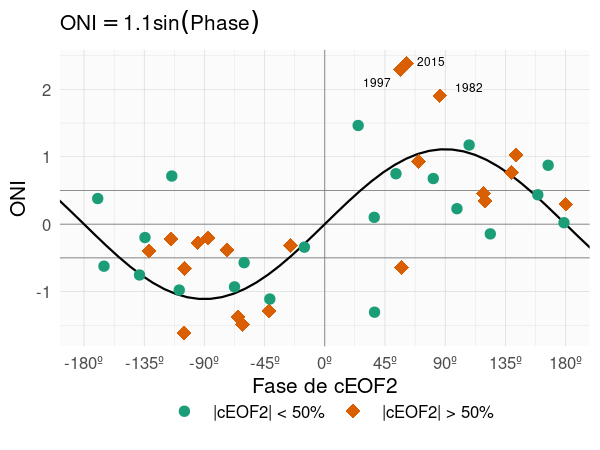
\includegraphics{figures/20-ceofs/enso-phase-1} 

}

\caption{Valores del ONI en SON y la fase del cEOF2 en el período 1979--2020. Los años en los cuales la magnitud del cEOF2 es mayor o menor que la mediana se muestran como diamantes naranja o círculos verdes respectivamente. La línea negra representa el ajuste ONI \textasciitilde{} sen(fase) computado por cuadrados mínimos pesados por la magnitud del cEOF2.}\label{fig:enso-phase}
\end{figure}

Para explorar la relación entre el forzante tropical y las fases del cEOF2 con más profundidad, la Figura \ref{fig:enso-phase} muestra la relación entre el ONI y la fase del cEOF2 para cada SON entre 1979 y 2020, destacando los años en los que la magnitud del cEOF2 está por encima de la mediana.
En los años con ONI positivo, la fase cEOF2 se sitúa mayoritariamente en torno a la fase de 90º; en los años con ONI negativo, en torno a la fase de -90º.
En las estaciones con ENSO neutro, la fase del cEOF2 es mucho más variable.
La línea negra de la Figura \ref{fig:enso-phase} es un ajuste sinusoidal de la relación entre el ONI y la fase del cEOF2.
El \(r^2\) correspondiente al ajuste es 0.57, estadísticamente significativo con p-valor \textless{} 0.001, lo que indica una relación aproximadamente sinusoidal entre estas dos variables.

\begin{figure}

{\centering 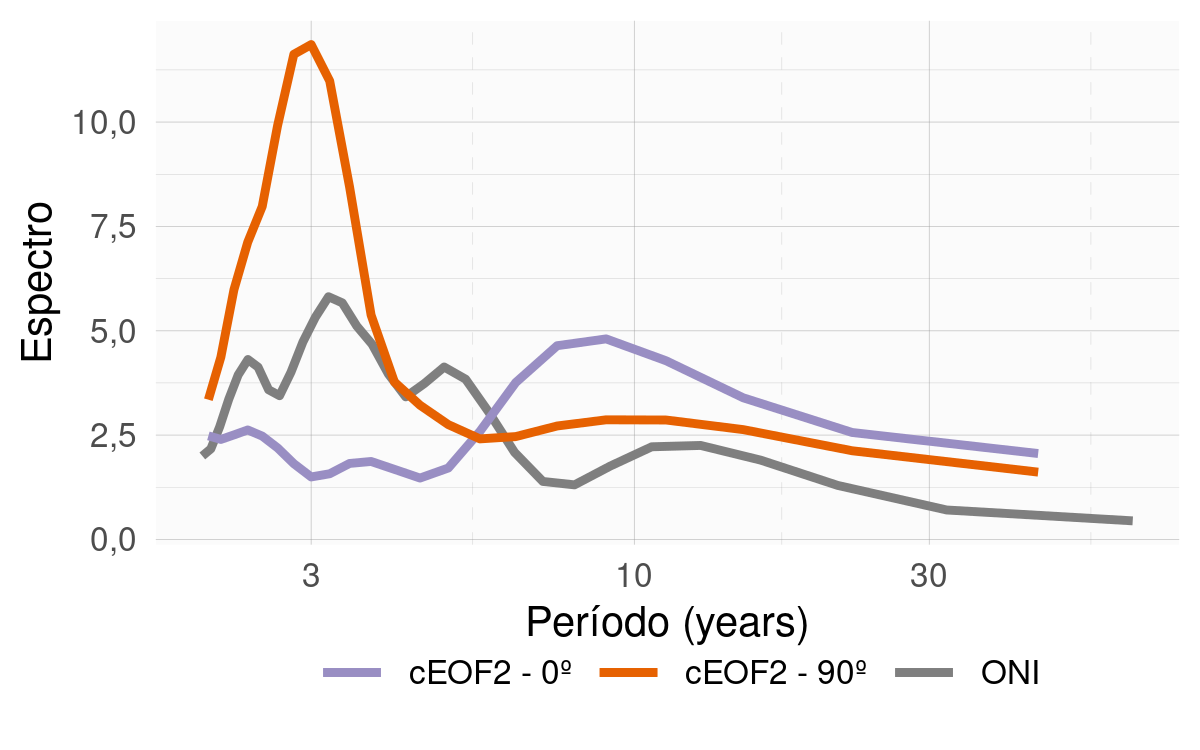
\includegraphics{figures/20-ceofs/fft-ceof-era5-1} 

}

\caption{Espectro de Fourier para cada fase del cEOF2 y del ONI.}\label{fig:fft-ceof-era5}
\end{figure}



Otra evidencia de la relación entre el ENSO y la fase del cEOF2 es que tanto el ONI como la fase de 90º del cEOF2 tienen un pico de periodicidad alrededor de 3 años (Fig. \ref{fig:fft-ceof-era5}.
Esto muestra que la principal escala de variabilidad de esta fase está íntimamente relacionada con el ENSO.

La correlación entre la magnitud absoluta del ONI y la amplitud del cEOF2 es 0.45 (CI: 0.17 -- 0.66).
Sin embargo, esta relación está determinada principalmente por los tres años con los eventos ENSO más intensos del periodo (2015, 1997, y 1982), los cuales coinciden con los tres años con la magnitud CEOF2 más intensa (no se muestra).
Si se eliminan esos años, la correlación deja de ser significativa (0.04 (CI: -0.28 -- 0.35)).
Además, incluso cuando utilizando todos los años, la correlación de Spearman -que es robusta frente a los valores atípicos- tampoco es significativa (0.2, p-valor = 0.21).
Por lo tanto, aunque la localización de las anomalías tropicales de la TSM parece tener un efecto en la definición de la fase del cEOF2, la relación entre la magnitud del cEOF2 y el ONI sigue siendo incierta y podría ser sólo evidente en eventos ENSO muy fuertes, que son escasos en el registro observacional histórico.

Concluimos que el tren de ondas representado por el cEOF2 es tanto parte de la variabilidad interna de la atmósfera extratropical como forzado por las TSM tropicales.
En el primer caso, el tren de ondas tiene poca preferencia de fase.
Sin embargo, cuando el cEOF2 es excitado por la variabilidad de la TSM tropical, tiende a permanecer fijo en la fase de 90º.



\begin{figure}

{\centering 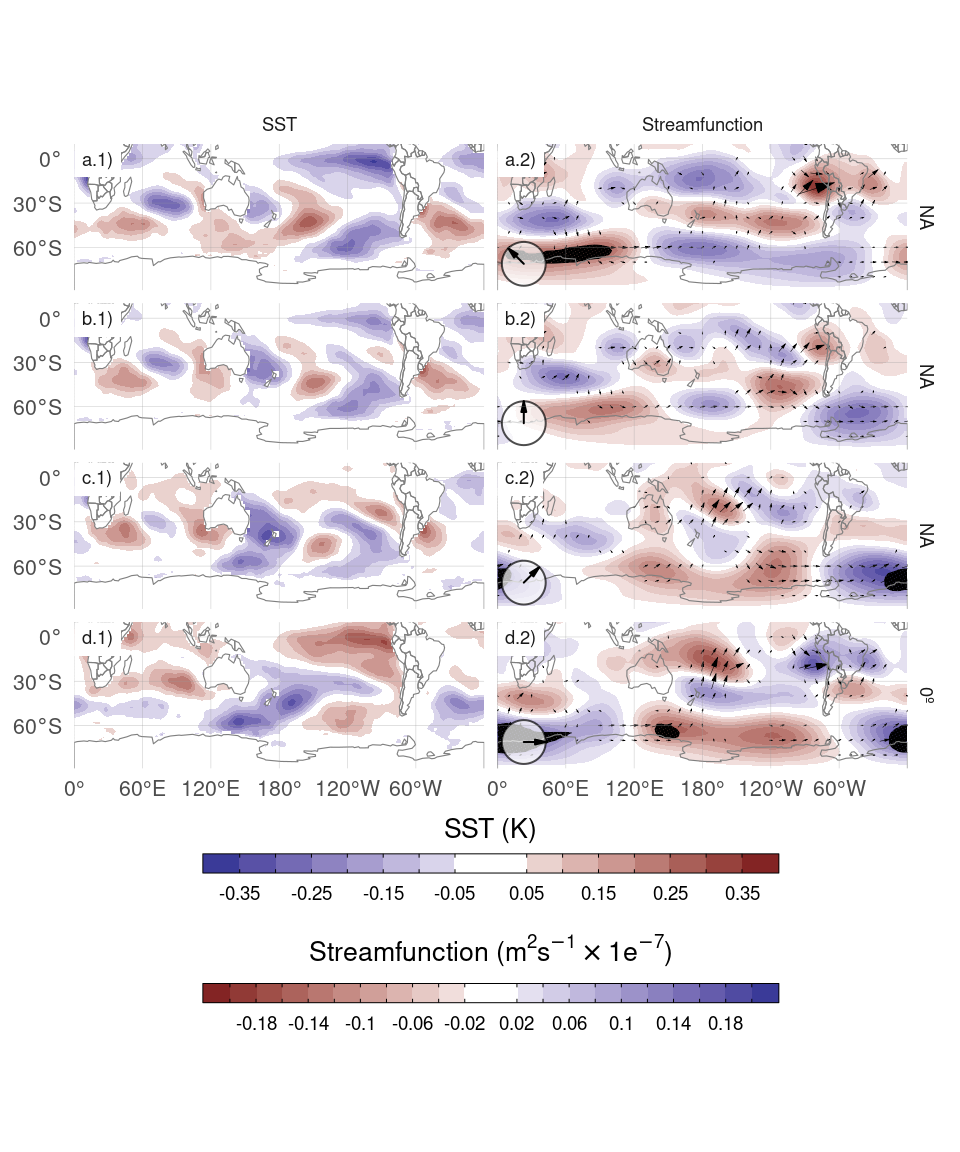
\includegraphics{figures/20-ceofs/sst-psi-1-1} 

}

\caption{Igual que la Figura~\ref{fig:sst-psi-2} pero para el cEOF1.}\label{fig:sst-psi-1}
\end{figure}

La Figura \ref{fig:sst-psi-1} muestra las mismas regresiones que la Figura \ref{fig:sst-psi-2} pero para el cEOF1.
Como anticipó la Figura \ref{fig:psi-sst-explained-variance}, el cEOF1 no está asociado a anomalías significativas de TSM ni de función corriente en los trópicos.
En vez de eso, las fases de 0º y 90º están asociadas a flujos de actividad de onda que se propagan zonalmente en los extratrópicos cerca de de 60ºS, excepto por un flujo hacia el ecuador desde la costa de la Antártida alrededor de 150ºE en la fase de 0º.
Esto sugiere que la variabilidad de cEOF1 está impulsada principalmente por la variabilidad interna de los extratrópicos.

\hypertarget{impactos}{%
\subsection{Impactos en superficie}\label{impactos}}

\begin{figure}

{\centering 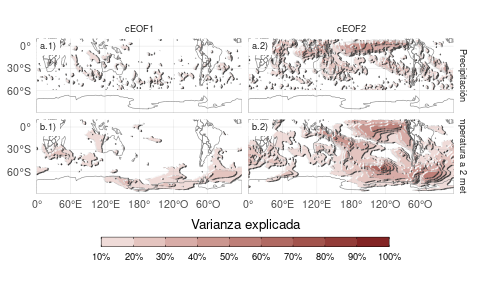
\includegraphics{figures/20-ceofs/pp-t2m-r2-1} 

}

\caption{Igual que la Figura \ref{fig:psi-sst-explained-variance} pero para Temperatura a 2 metros y precipitación.}\label{fig:pp-t2m-r2}
\end{figure}



La Figura \ref{fig:pp-t2m-r2} muestra la varianza de la temperatura a 2 metros y de la precipitación explicada por cada cEOF.

La varianza explicada por el cEOF1 para ambas variables es muy baja en la mayoría de las regiones, excepto para el extremo norte de la Península Antártica, el norte del Mar de Weddell y la costa del Mar de Ross (Fig.\ref{fig:pp-t2m-r2}a.1).

Por otro lado, la varianza explicada cEOF2 es superior al 50\% en algunas regiones para ambas variables (Fig. \ref{fig:pp-t2m-r2} columna 2).
Para la temperatura de 2 metros, hay valores altos en el Pacífico tropical y en la región que forma un arco entre Nueva Zelanda y el Atlántico Sur.
Sobre los continentes, hay valores moderados de alrededor del 30\% de varianza explicada en el sur de Australia, el sur de Sudamérica y la Península Antártica.
En cuanto a las precipitaciones, los valores son elevados en los trópicos.
En latitudes más altas, se observan valores moderados sobre el este de Australia y algunas regiones del sur de Sudamérica.

Dado que el cEOF1 tiene una señal relativamente débil en las variables de superficie exploradas, sólo nos centraremos en la influencia del cEOF2.
En la Figura \ref{fig:pp-temp-2} se muestran mapas de regresión de las anomalías de temperatura a 2 metros (columna 1) y precipitación (columna 2) sobre diferentes fases del cEOF2 normalizado.



\begin{figure}

{\centering 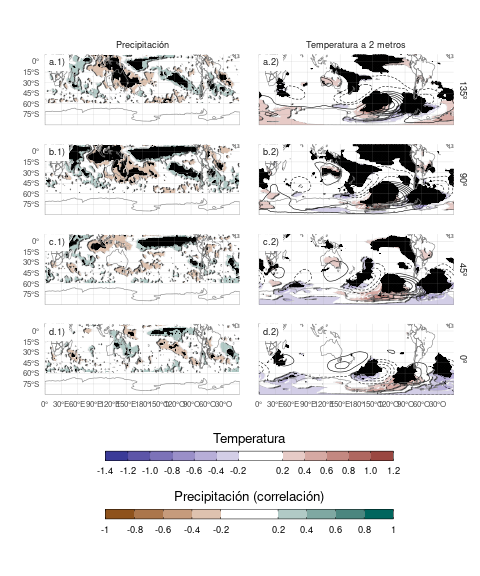
\includegraphics{figures/20-ceofs/pp-temp-2-1} 

}

\caption{Regresión de la temperatura de 2 metros (K, sombreado) y la altura geopotencial de 850 hPa (m, contornos) (columna 1), y la precipitación (correlación, columna 2) sobre diferentes fases de cEOF2. Para el trimestre SON del periodo 1979--2020. Áreas con puntos marcan regiones donde el p-valor es menor que 0.01 ajustado por FDR.}\label{fig:pp-temp-2}
\end{figure}

Las anomalías de temperatura asociadas a la fase de 90º del cEOF2 (Fig.~\ref{fig:pp-temp-2}.b1) muestran valores positivos en el Pacífico tropical, coherentes con las anomalías de TSM asociadas a esta misma fase (Fig.~\ref{fig:sst-psi-2}.b1).
En latitudes más altas existe un patrón ondulatorio de valores positivos y negativos que coincide con los nodos de los patrones de regresión de la altura geopotencial de 850 hPa.
Esto es coherente con las anomalías de temperatura producidas por la advección meridional de temperatura por los vientos meridionales derivados del equilibrio geostrófico.
Sobre los continentes, las fase de 90º (Fig.\ref{fig:pp-temp-2}b.1) está asociada a anomalías de temperatura positiva en el sur de Australia y anomalías de regresión negativa en el sur de Sudamérica y la Península Antártica, que son resultado del tren de ondas descrito anteriormente.

Las anomalías de temperatura asociadas a la fase de 0º (Fig.\ref{fig:pp-temp-2}d.1) son menos extensas y se limitan a latitudes medias y altas.
Sobre los continentes, las regresiones de las anomalías de temperatura no son significativas, excepto las anomalías positivas cerca de la Península Antártica.

Las anomalías de precipitación tropicales asociadas con el 90º cEOF2 son fuertes, con anomalías positivas en el Pacífico central y el Índico occidental, y anomalías negativas en el Pacífico oriental (Fig.\ref{fig:pp-temp-2}b.2).
Este campo es consistente con el mapa de regresión de la TSM (Fig.\ref{fig:pp-temp-2}b.1) ya que las anomalías positivas de la TSM potencian la convección tropical y las anomalías negativas de la TSM la inhiben.

En los extratrópicos, la fase de 90º del cEOF2 se asocia a condiciones más secas sobre el este de Australia y el océano circundante, que es una señal similar a la asociada al ENSO (Cai et~al. 2011).
Sin embargo, esta es la fase más fuertemente correlacionada con la precipitación en esa zona.
La fase de 135º (una intermedia 90º y 180º) está correlacionada más intensa y extensamente con la precipitación sobre Australia y Nueva Zelanda.
La influencia del cEOF2 en la precipitación australiana podría estar relacionada más con los impactos directos de las anomalías de la TSM en los océanos circundantes que en el patrón de teleconexión representado por el cEOF2.

Sobre Sudamérica, la fase de 90º del cEOF2 está correlacionada positivamente con la precipitación en el sudeste de Sudamérica (SESA) y el centro de Chile, y negativamente en el este de Brasil.
Este campo de correlación coincide con la señal de ENSO la precipitación de primavera (p.e. Cai et~al. 2020).

Los coeficientes de correlación entre las anomalías de precipitación y la fase de 0º del cEOF2 (Fig.~\ref{fig:pp-temp-2}d.2) son más débiles que para la fase de 90º.
Hay una correlación positiva residual en el Pacífico oriental ecuatorial y pequeñas correlaciones positivas, no estadísticamente significativas, sobre el este de Australia y negativas sobre Nueva Zelanda.

\hypertarget{conclusiuxf3n}{%
\section{Conclusión}\label{conclusiuxf3n}}

Los cEOF identificados en este capítulo logran representar características importantes de la circulación zonalmente asimétrica del hemisferio sur.
El cEOF1 captura principalmente la onda 1 en la estratósfera mientras que el cEOF2 representa la onda 3 con un máximo de amplitud en el Pacífico sur.

El cEOF2 está asociado a forzantes tropicales y el tren de ondas que representa se asemeja a los modos PSA y la circulación asociada a ambos cEOF tiene características similares al SAM.
Antes de estudiar estas relaciones en más detalle, es necesario estudiar el SAM y entender sus características zonalmente simétricas y asimétricas.

\hypertarget{asymsam}{%
\chapter{Estructura simétrica y asimétrica del Modo Anular del Sur}\label{asymsam}}

\hypertarget{introducciuxf3n-1}{%
\section{Introducción}\label{introducciuxf3n-1}}

Como se explicó en la introducción, el patrón espacial del Modo Anular del Sur (SAM) suele describirse en términos de la circulación zonalmente simétrica, sin embargo este patrón tiene asimetrías zonales significativas.
Por otro lado, en el capítulo anterior se observó que algunas fases de los cEOFs están asociadas con patrones tipo SAM en algunos niveles.

El objetivo de este capítulo es, por tanto, describir los componentes zonalmente asimétricos y simétricos de la variabilidad del SAM.
En primer lugar, se propone una metodología que proporciona, para cada nivel, sendos índices que pretenden captar de forma independiente la variabilidad de la componente del SAM simétrica y asimétrica, respectivamente.
Luego se evaluó su estructura vertical y su coherencia, así como su variabilidad temporal y sus tendencias.
A continuación se estudiaron los patrones espaciales asociados a la variabilidad exclusiva de cada índice centrándose en 50 hPa como nivel estratosférico y 700 hPa como nivel troposférico.
Por último, se investigaron las relaciones del SAM a 700 hPa con las anomalías de temperatura y precipitación.

\hypertarget{muxe9todos-3}{%
\section{Métodos}\label{muxe9todos-3}}

\hypertarget{regresiuxf3n-segmentada}{%
\subsection{Regresión segmentada}\label{regresiuxf3n-segmentada}}

En la literatura suelen usarse composiciones de eventos positivos y negativos definidos a partir de un determinado límite para para estimar campos la asociación de una variable con la parte positiva y negativa de un índice.
Esta metodología no utiliza todos los datos eficientemente y los resultados son difíciles de interpretar si el valor absoluto típico del índice es mayor para casos positivos que negativos o viceversa.
En vez de eso, en este capítulo calculamos los campos asociados al SAM positivo y negativo utilizando regresión lineal segmentada.
Ésta consiste en ajustar un modelo lineal a tramos con continuidad en cada segmento como se ilustra en la Figura \ref{fig:segmentada-ejemplo} con datos sintéticos.

\begin{figure}

{\centering 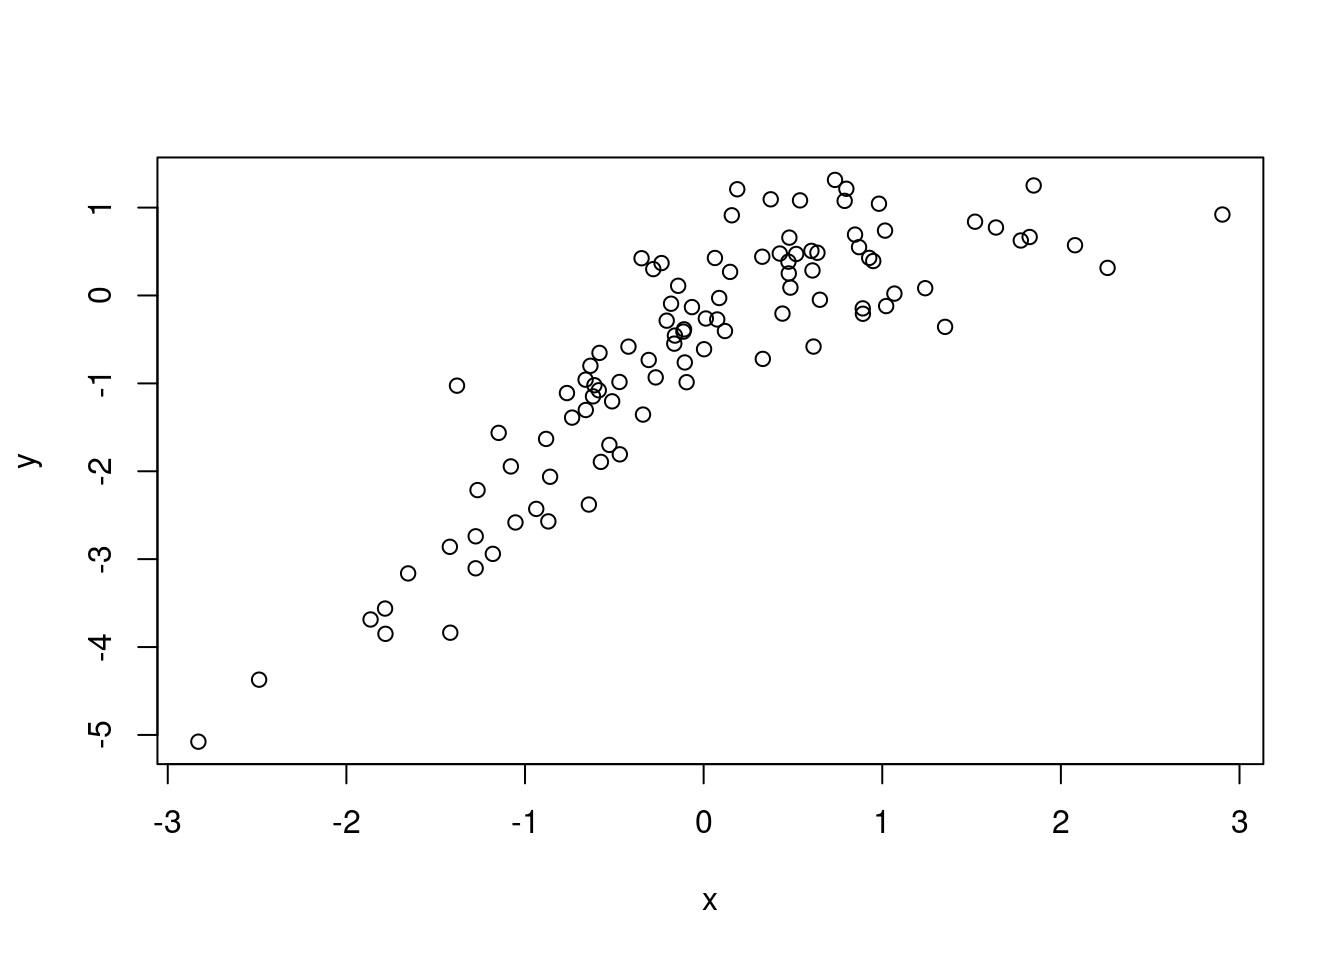
\includegraphics{figures/30-sam/segmentada-ejemplo-1} 

}

\caption{Ejemplo de regresión segmentada. La relación entre X e Y es lineal pero con distinta pendiente para valores de X positivos y negativos.}\label{fig:segmentada-ejemplo}
\end{figure}



Para obtener las pendientes asociadas a la relación lineal para cada signo, ajustamos la ecuación

\[
Y_i = \alpha X_i + \beta X_iI_{X\le 0} + X_0 + \epsilon_i
\]

donde \(Y\) e \(X\) son las variables dependiente e independiente respectivamente, \(\alpha\) es la pendiente asociada a los valores positivos de \(X\), \(\beta\) es la diferencia entre la pendiente asociada a valores positivos y negativos de \(X\), \(I_{X\le 0}\) es la función indicador que es 1 cuando \(X\le0\) y 0 cuando \(X>0\), y \(X_0\) y \(\epsilon_i\) son la constante y los términos de error.
El coeficiente asociado a valores negativos de X es \(\beta - \alpha\).

Esta metodología utiliza todos los datos disponibles.
Además, dado que \(\beta\) es la diferencia en la pendiente entre valores positivos y negativos, es posible calcular la insignificancia estadística de la misma.

\hypertarget{definition-of-indices}{%
\subsection{Definición de los índices}\label{definition-of-indices}}

El SAM suele definirse como el primer EOF de las anomalías de la presión al nivel del mar o de la altura geopotencial en niveles bajos (Ho, Kiem y Verdon-Kidd 2012).
Siguiendo a Baldwin (2001), ampliamos esa definición verticalmente y utilizamos el término SAM para referirnos al primer EOF de las anomalías mensuales de altura geopotencial al sur de 20º S en cada nivel.

Para separar la componente zonalmente simétrica y asimétrica del SAM, calculamos la media zonal y las anomalías del patrón espacial completo del SAM, como muestra en la Figura \ref{fig:method} en 700 hPa.
La señal espacial completa (\(\mathrm{EOF_1}(\lambda, \phi)\)) es la suma de la componente zonalmente asimétrica (\(\mathrm{EOF_1^*}(\lambda, \phi)\)) y la simétrica (\([\mathrm{EOF_1}](\lambda, \phi)\)).
A continuación, calculamos el índice SAM, el índice SAM asimétrico (A-SAM) y el índice SAM simétrico (S-SAM) como los coeficientes de la regresión de cada campo de altura geopotencial mensual sobre los respectivos patrones (ponderando por el coseno de la latitud).
Finalmente, normalizamos los tres índices dividiéndolos por la desviación estándar del índice SAM en cada nivel.
Como resultado, las magnitudes entre los índices son comparables.
Sin embargo, sólo el índice SAM tiene desviación estándar unitaria por definición.
La varianza explicada por cada patrón se utiliza como indicador del grado de simetría o asimetría zonal de cada campo mensual.
Para cuantificar la coherencia entre las series temporales correspondientes a distintos índices o al mismo índice en distintos niveles, calculamos la correlación temporal entre ellas.



\begin{figure}

{\centering 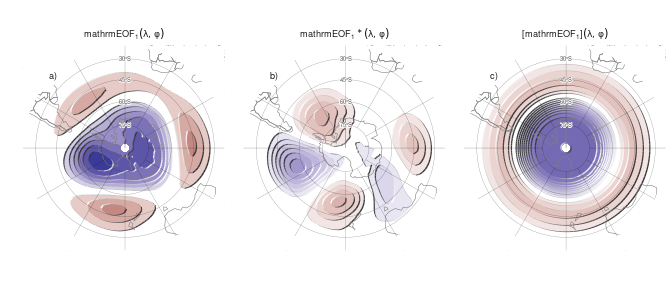
\includegraphics{figures/30-sam/method-1} 

}

\caption{Patrones espaciales del primer EOF de la altura geopotencial en 700 hPa para el período 1979--2020. (a) Campo completo, (b) componente zonalmente asimétrica y (c) componente zonalmente simétrica. Unidades arbitrarias con valores negativos en azul y negativos en azul.}\label{fig:method}
\end{figure}

\hypertarget{limitaciones}{%
\subsubsection{Limitaciones}\label{limitaciones}}

El método supone linealidad en las componentes del SAM.
Es decir, supone que los patrones de anomalías asociadas a valores positivos de cada componente del SAM son similares pero de signo opuesto a las asociadas a la fase valores negativos y de magnitud proporcional a la magnitud del índice.
Las composiciones de Fogt, Jones y Renwick (2012) (su Figura 4) sugieren que esto podría no ser del todo válido, aunque gran parte de esa aparente no linealidad podría deberse a la naturaleza heterogénea de los años seleccionados para construir las composiciones y a incertidumbre muestral.

Para poner esta suposición a prueba, calculamos la regresión segmentada de las anomalías zonales de altura geopotencial con el índice SAM para cada signo del SAM.
Las Figuras \ref{fig:sign-regression-50} y \ref{fig:sign-regression-700} muestran los campos de regresión en 50 y 700 hPa divididos por trimestres.
Se puede observar que en casi todas las estaciones y ambos niveles, los campos de regresión de SAM positivo y negativo son similares entre ellos.
Este análisis cualitativo se confirma por el análisis cuantitativo de al observar que el \(r^2\) (representando la correlación espacial al cuadrado) tienen valores entre 0.7 y 0.9, indicando alta similaridad.
A su vez, también es similar la intensidad de los coeficientes de correlación, indicando un buen cumplimiento de la hipótesis de linealidad.



\begin{figure}

{\centering 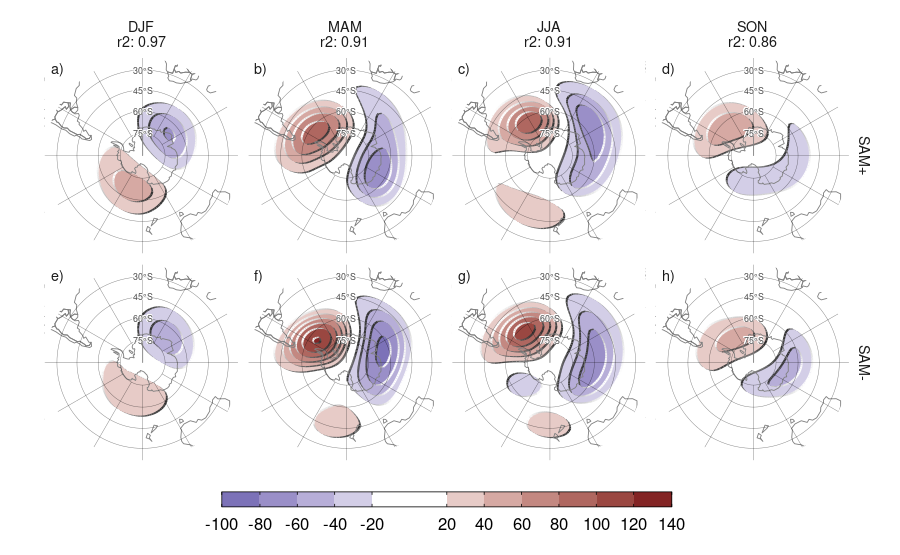
\includegraphics{figures/30-sam/sign-regression-50-1} 

}

\caption{Regresión segmentada de la anomalía zonal de altura geopotencial en 50 hPa con el índice SAM para cada signo para el período 1979--2020. La correlación espacial al cuadrado entre cada campo en cada estación se detalla debajo de la estación. Áreas con puntos marcan regiones donde el p-valor de la diferencia entre el signo positivo y el negativo es menor que 0.01 ajustado por FDR (no hay áreas).}\label{fig:sign-regression-50}
\end{figure}



\begin{figure}

{\centering 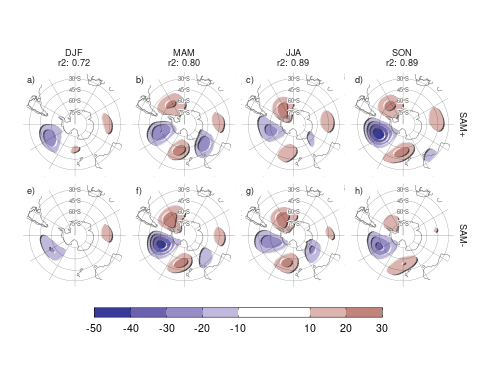
\includegraphics{figures/30-sam/sign-regression-700-1} 

}

\caption{Igual que la Figura \ref{fig:sign-regression-50} pero para 700 hPa.}\label{fig:sign-regression-700}
\end{figure}

Al realizar el análisis EOF utilizando los datos de todos los meses también estamos asumiendo que la estructura del SAM es la misma en todas las estaciones.
La Figura \ref{fig:season-regression} muestra la regresión del SAM para cada trimestre del año y la significancia estadística de la diferencia entre cada estación y SON.

En 50 hPa (Fig. \ref{fig:season-regression} fila a), los patrones del SAM para MAM y JJA son muy similares a SON, con correlación espacial cuadrada mayor a 0.75.
En estas tres estaciones, el SAM en 50 hPa se asocia a una onda planetaria 1 con su centro negativo en 60ºO.
El patrón de JJA tiene algunas diferencias significativas con respecto a SON, principalmente un corrimiento e intensificación de la anomalía negativa de la onda.
El patrón de DJF, en cambio, es muy distinto; la onda 1 tiene su mínimo cerca de 180ºO y está más retraída a latitudes altas.
Además, su correlación espacial es esencialmente nula.

En 700 hPa (Fig. \ref{fig:season-regression} fila b), las cuatro estaciones tienen patrones bastante similares, prácticamente sin diferencias estadísticamente significativas con respecto a SON y con correlaciones cuadradas mayores a 0.6.
El patrón de DJF el más distinto, siendo similar a SON pero menos intenso.
Esto es consistente con los resultados de Fogt y Marshall (2020).

Estos resultados sugieren que la suposición de estabilidad estacional se cumple excepto por DJF en la estratósfera.
Esto indica que hay que tener cuidado en la interpretación del SAM asimétrico en DJF en la estratosfera ya que el patrón de SAM asimétrico impuesto por la metodología no coincide con el patrón de SAM asimétrico que se obtendría considerando únucamente este trimestre.



\begin{figure}

{\centering 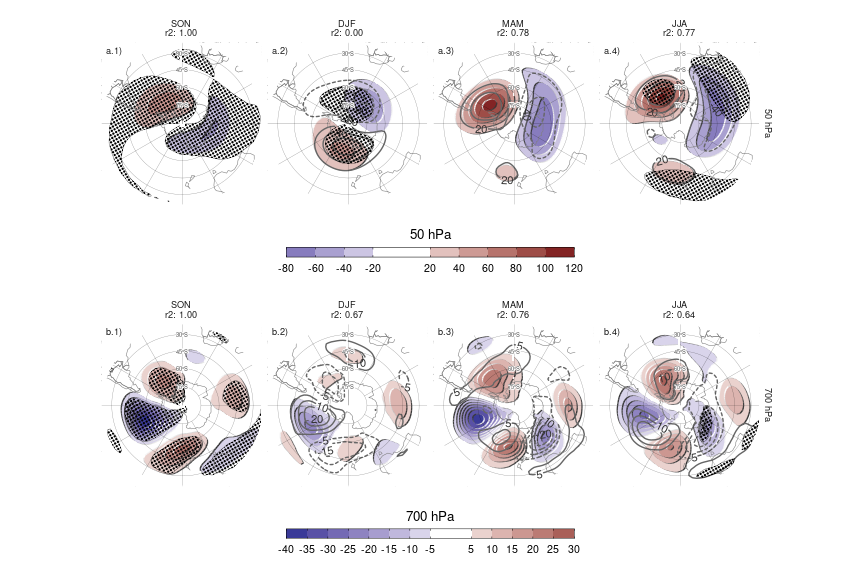
\includegraphics{figures/30-sam/season-regression-1} 

}

\caption{Regresión múltiple de las anomalías zonales de altura geopotencial para cada estación. El sombreado muestra la regresión de cada estación y los contornos grises, la diferencia de cada estación con respecto a SON (valores negativos en línea punteada y positivos en línea sólida). La correlación espacial al cuadrado entre cada campo y el campo de SON se detalla debajo de la estación. Áreas con puntos marcan regiones donde el p-valor es menor que 0.01 ajustado por FDR, donde para estaciones distintas a SON, marca el p-valor de la diferencia respecto a SON.}\label{fig:season-regression}
\end{figure}

El método también asume que el patrón zonalmente asimétrico del SAM permanece estacionario a lo largo del periodo considerado.
Silvestri y Vera (2009) sugiere que este podría no ser el caso entre 1958 y 2004.
Para probar esta suposición, calculamos el SAM para las dos mitades del periodo (1979 a 1998 y 1999 a 2020), que se muestran en la Figura \ref{fig:sam-period}.
Las diferencias entre los dos periodos parecen ser relativamente pequeñas, tanto en la troposfera como en la estratosfera.



\begin{figure}

{\centering 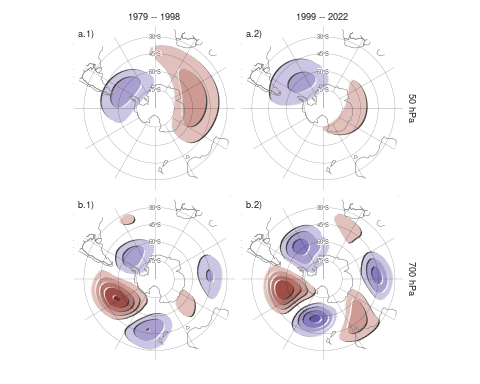
\includegraphics{figures/30-sam/sam-period-1} 

}

\caption{Patrón espacial del primer EOF computado para el período 1979 -- 1998 (columna 1) y 1999 -- 2020 (columna 2) para 50 hPa (fila a) y 700 hPa (fila b). Unidades arbitrarias con valores negativos en azul y negativos en azul.}\label{fig:sam-period}
\end{figure}

\hypertarget{resultados-2}{%
\section{Resultados}\label{resultados-2}}

\hypertarget{temporal}{%
\subsection{Evolución temporal}\label{temporal}}



\begin{figure}

{\centering 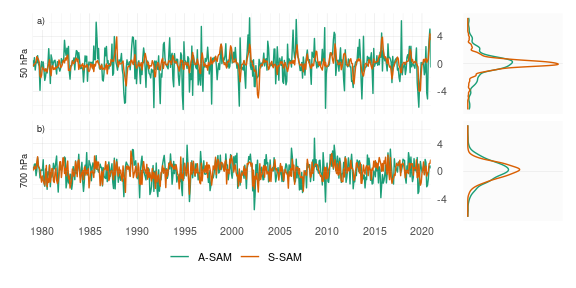
\includegraphics{figures/30-sam/asymsam-timeseries-1} 

}

\caption{Serie temporal de A-SAM y S-SAM en 50 hPa (panel a) y 700 hPa (panel b). A la derecha, la densidad de probabilidad de cada índice. Las series están estandarizadas por el desvío estándar del SAM en cada nivel.}\label{fig:asymsam-timeseries}
\end{figure}

Primero evaluamos la evolución temporal del A-SAM y S-SAM.
La Figura \ref{fig:asymsam-timeseries} muestra las series temporales en 700 hPa y 50 hPa y sus correspondientes estimaciones de densidad.
Seleccionamos estos dos niveles como representativos de la variabilidad troposférica y estratosférica respectivamente.
Como se muestra a continuación, las variabilidades de ambos índices son muy coherentes dentro de cada región de la atmósfera, por lo que es razonable tomar un nivel como representativo de cada capa.

La variabilidad mes a mes es evidente para ambos índices, con variaciones ruidosas en las frecuencias bajas.



\begin{figure}

{\centering 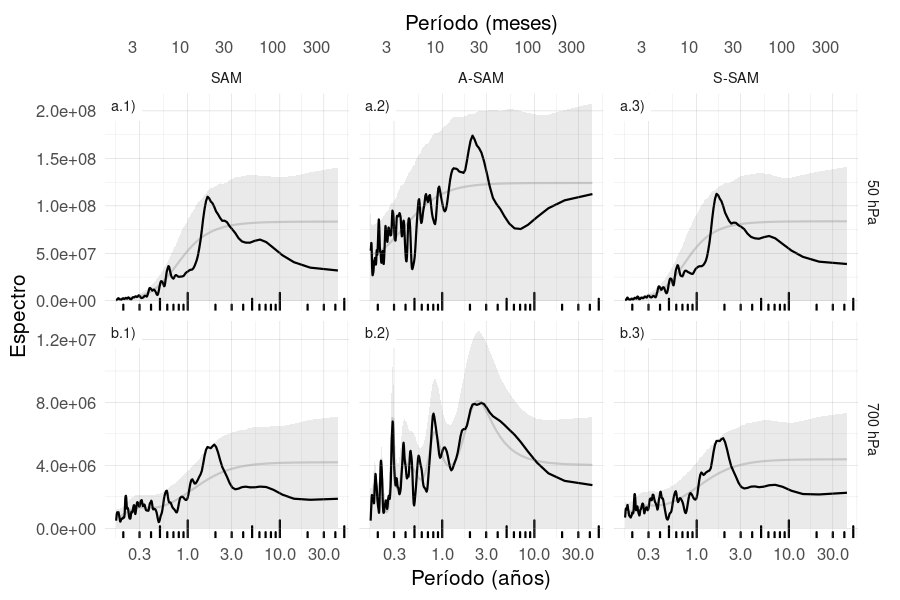
\includegraphics{figures/30-sam/spectrum-1} 

}

\caption{Espectro de cada serie temporal suavizada. El sombreado indica el intervalo de confianza del 95\% del espectro nulo calculado usando bootstrap tomando 5000 simulaciones de un modelo autoregresivo ajustado a los datos. La línea gris indica la amplitud promedio teórica del modelo autoregresivo. Para el período 1979--2020.}\label{fig:spectrum}
\end{figure}

Los espectros de estas series temporales se muestran en la Figura \ref{fig:spectrum}.
El S-SAM estratosférico varía fuertemente con un periodo entre 10 y 30 meses (Fig. \ref{fig:spectrum} a.3).
En el periodograma del S-SAM troposférico (Fig.\ref{fig:spectrum} b.3) se aprecia un pico local en un rango de frecuencias similar, aunque no es estadísticamente significativo.
Esta banda de periodicidad está alrededor del rango de periodicidad de la Oscilación Cuasi-Bienal (QBO, por su siglas en inglés, Baldwin et~al. (2001)) y es consistente con (Vasconcellos, Mattos-Gava y Sansigolo 2022), quien encontró que el SAM y la QBO comparten una alta potencia común significativa alrededor de la banda de 2 años.
El hecho de que esta periodicidad no sea evidente en el índice A-SAM, también es consistente con sus composiciones de anomalías de altura geopotencial durante la QBO oriental y occidental, que muestran un monopolo bastante simétrico sobre la Antártida.
En la troposfera, el pico de variabilidad más significativo se encuentra en A-SAM en torno a 36 meses.

Las series temporales A-SAM y S-SAM parecen estar correlacionadas.
Además, observando los extremos en la estratosfera, la serie S-SAM parece ir por detrás de la serie A-SAM (véanse, por ejemplo, los eventos positivos de finales de 1987).
La Figura \ref{fig:cor-lev} muestra la correlación entre A-SAM y S-SAM en cada nivel para los retrasos cero y -1.
Los valores de las correlaciones instantáneas entre A-SAM y S-SAM son relativamente constantes en toda la troposfera, fluctuando entre 0.38 y 0.44.
Las correlaciones con desfase de un mes son igualmente constantes pero muy reducidas.
En la estratosfera, las correlaciones instantáneas caen a un mínimo de 0.28 en 20 hPa y luego aumentan nuevamente monotónicamente con la altura hasta el nivel más alto del reanálisis (aunque los resultados cerca de la parte superior de los modelos deben interpretarse con cuidado).
Al mismo tiempo, las correlaciones con un mes de defasaje aumentan con la altura.
Por lo tanto, el índice A-SAM estratosférico tiende a preceder al índice S-SAM.



\begin{figure}

{\centering 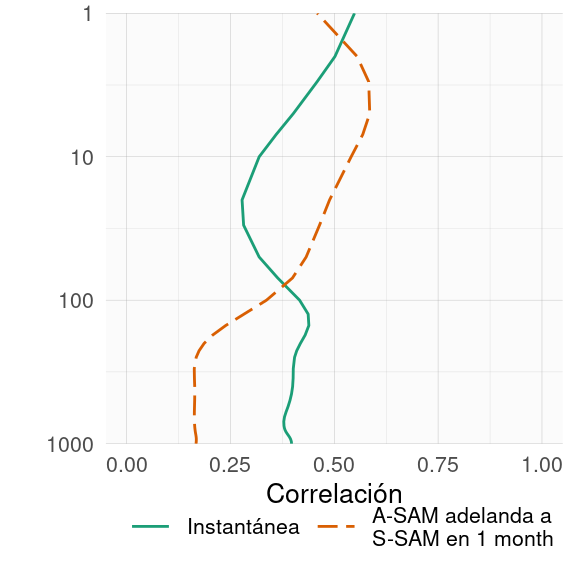
\includegraphics{figures/30-sam/cor-lev-1} 

}

\caption{Correlación instantánea y con un defasaje de 1 mes entre S-SAM y A-SAM para el período 1979--2020.}\label{fig:cor-lev}
\end{figure}



\begin{figure}

{\centering 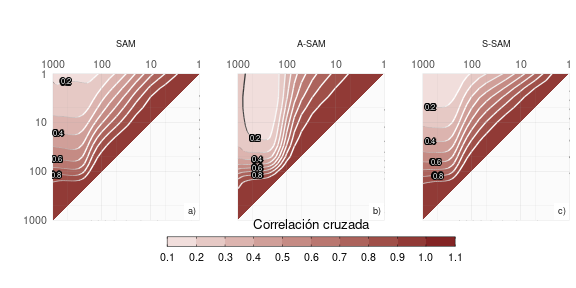
\includegraphics{figures/30-sam/cross-correlation-1} 

}

\caption{Correlación cruzada entre niveles para el índice SAM (a), A-SAM (b) y S-SAM (c) para el período 1979--2020.}\label{fig:cross-correlation}
\end{figure}

La Figura \ref{fig:cross-correlation} muestra la correlación cruzada (lag cero) entre niveles para los índices SAM, A-SAM y S-SAM.
Para el SAM (Fig. \ref{fig:cross-correlation}a), los valores altos por debajo de 100 hPa reflejan la coherencia vertical en toda la troposfera.
Por encima de 100 hPa, la correlación entre niveles disminuye más rápidamente, lo que indica una variabilidad menos coherente.
Sin embargo, las correlaciones entre los niveles troposféricos y los niveles estratosféricos bajos y medios siguen siendo relativamente altas (por ejemplo, más de 0,4 entre los niveles troposféricos y los niveles por debajo de 30 hPa).
A-SAM y S-SAM (Fig. \ref{fig:cross-correlation}b y c, respectivamente) comparten un alto nivel de coherencia similar en la troposfera, pero difieren en su comportamiento estratosférico.
La coherencia estratosférica es mayor para el A-SAM que para el S-SAM.
El S-SAM estratosférico tiene una conexión con el S-SAM troposférico algo más intensa que el A-SAM estratosférico con el A-SAM troposférico.



\begin{figure}

{\centering 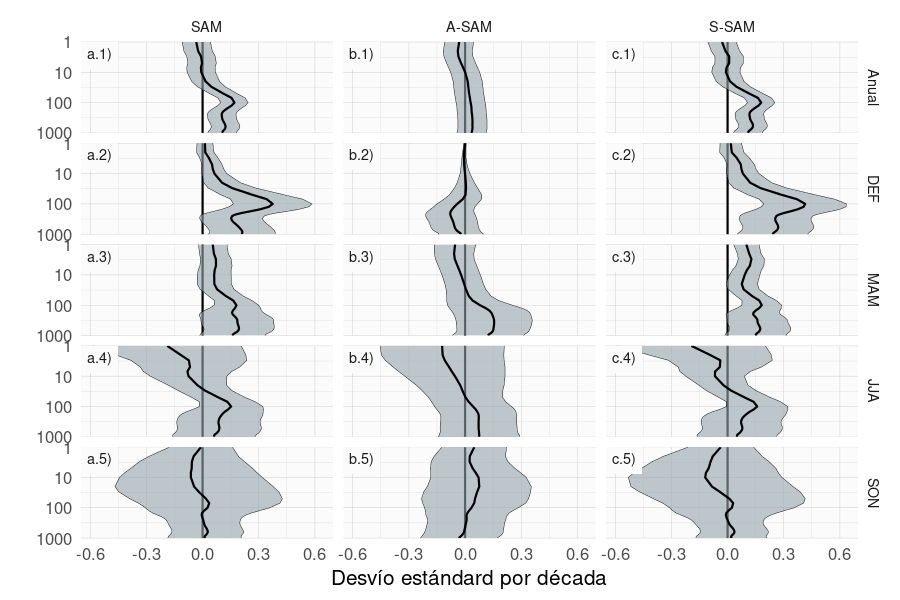
\includegraphics{figures/30-sam/trends-1} 

}

\caption{Tendencias lineales (en desvio estandard por década) del SAM (columna a), A-SAM (columna b) y S-SAM (columna c) para cada nivel usando datos del todo el año (fila 1) y promedios estacionales (filas 2 a 5) para el período 1979--2020. El sombreado indica el intervalo de confianza de 95\%.}\label{fig:trends}
\end{figure}

Evaluamos las tendencias lineales para cada uno de los índices para el periodo 1979--2020 en cada nivel para el año completo y separado por trimestres (Fig. \ref{fig:trends}).
El índice SAM presenta una tendencia positiva estadísticamente significativa (Fig. \ref{fig:trends}a.1) en todos los niveles entre 1000 hPa y aproximadamente 50 hPa, con un máximo en 100 hPa.
Las tendencias estacionales (Fig. \ref{fig:trends} columna a) indican que las tendencias son significativas sólo en verano y marginalmente en otoño.
Esto es consistente con los resultados de estudios previos, los cuales documentaron tendencias positivas en verano, menores en otoño y ninguna tendencia en las demás estaciones (por ejemplo, Fogt y Marshall (2020) y sus referencias) utilizando índices del SAM basados en la circulación en o cerca de superficie.

Al separar la señal SAM en sus partes asimétrica y simétrica, no sólo podemos ver que estas tendencias se deben casi por completo al componente simétrico (comparar columnas b y c Figura \ref{fig:trends}), sino que en algunos casos las tendencias se vuelven más claras.
En verano, A-SAM tiene una tendencia negativa estadísticamente no significativa en la troposfera media que oculta la tendencia en el índice SAM; como resultado, las tendencias calculadas utilizando sólo la componente simétrica son más intensas (comparar la región sombreada en la Figura \ref{fig:trends}a.2 y c.2).
En otoño, el índice S-SAM revela una tendencia positiva estadísticamente significativa en la estratosfera que no es significativa utilizando el índice SAM.

Una tendencia positiva en el índice S-SAM y ninguna tendencia en el índice A-SAM podría sugerir en un primer momento una tendencia hacia un SAM más simétrico.
Sin embargo, un S-SAM muy negativo con tendencia a un S-SAM menos negativo se traduciría en una tendencia positiva del S-SAM pero en una SAM más asimétrica.



\begin{figure}

{\centering 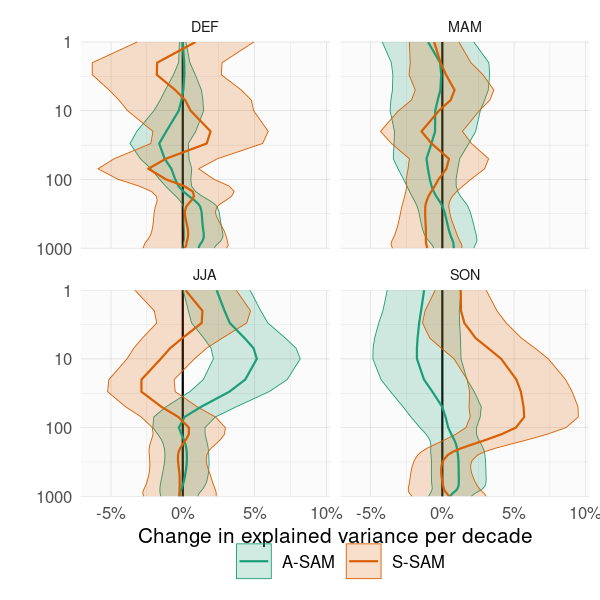
\includegraphics{figures/30-sam/r-squared-trend-1} 

}

\caption{Tendencias lineales (en porcentaje por década) de la varianza explicada por el A-SAM y el S-SAM en cada nivel para cada trimestre en el período 1979--2020. El sombreado indica el intervalo de confianza del 95\%.}\label{fig:r-squared-trend}
\end{figure}

Para estudiar la cuestión de si el SAM se está volviendo más o menos asimétrica, mostramos las tendencias de la varianza explicada de cada índice para cada trimestre en la Figura \ref{fig:r-squared-trend}.
En la troposfera, la única tendencia significativa es la de DJF, en la que el A-SAM tiene una tendencia positiva de alrededor del 2\% por década, lo que sugiere que el DJF SAM se ha vuelto más asimétrico en el período de 1979 a 2020 Fogt, Jones y Renwick (2012) observó un cambio de una SAM más asimétrica antes de 1980 a una SAM más simétrica después de 1980, pero nuestro periodo de estudio (1979--2020) nos impide detectar ese cambio.
Sin embargo, debido a la naturaleza atípica de la componente asimétrico del SAM durante la DJF (Sección \ref{definition-of-indices}), esto debe tomarse sólo como una evidencia preliminar.
La otra tendencia significativa se da en la estratosfera durante SON, donde hay una tendencia positiva en la varianza explicada por la S-SAM de aproximadamente un 4\% por década.
Este cambio podría ser el resultado del forzamiento provocado por el agotamiento del ozono.

\hypertarget{spatial}{%
\subsection{Patrones espaciales}\label{spatial}}



\begin{figure}

{\centering 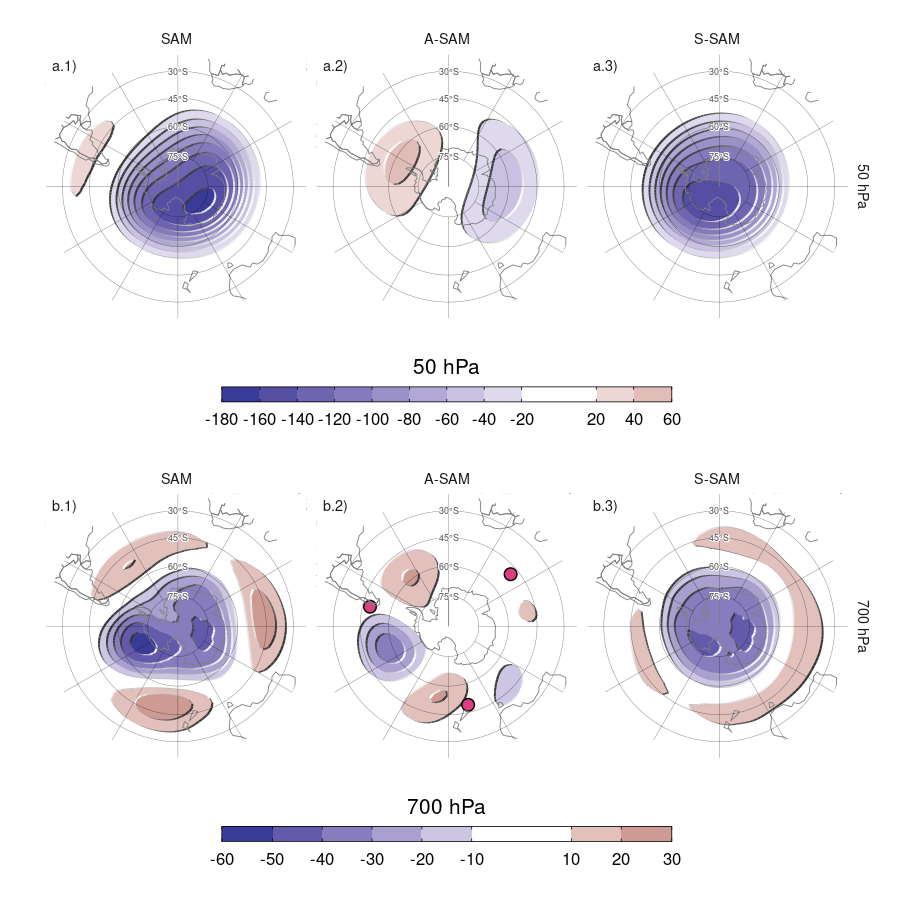
\includegraphics{figures/30-sam/2d-regr-1} 

}

\caption{Regresión de altura geopotencial (metros) en 50 hPa (fila a) y 700 hPa (fila b) con el SAM (columna 1), A-SAM (columna 2) y S-SAM (columna 3) para el período 1979--2020. Los puntos en panel b.2 indican la posición de los puntos de referencia usados por Raphael (2004) para calcular su índice de la onda zonal 3.}\label{fig:2d-regr}
\end{figure}

A continuación calculamos la regresión espacial de las anomalías de altura geopotencial sobre los índices SAM, A-SAM y S-SAM en los niveles de 50 hPa y 700 hPa (Fig. \ref{fig:2d-regr}).
Los coeficientes de regresión de la columna 1 de la Figura \ref{fig:2d-regr} se calcularon utilizando el índice del SAM.
Los coeficientes de regresión de las columnas 2 y 3 se calcularon mediante regresión múltiple utilizando los índices A-SAM y S-SAM al mismo tiempo, de manera que deben interpretarse como los patrones asociados a cada índice, eliminando la variabilidad (linealmente) explicada por el otro.

En la estratosfera, el patrón espacial asociado al SAM está claramente dominado por un monopolo que no está centrada en el Polo Sur (Fig. \ref{fig:2d-regr}a.1).
El patrón asociado a la parte asimétrica se caracteriza por una estructura de onda-1 con centros sobre el Pasaje de Drake en el Hemisferio Occidental y el Mar de Davis en el Hemisferio Oriental.
Este eje se alinea con el defasaje del monopolo del SAM.
Finalmente, el patrón asocaido al S-SAM, es un monopolo más simétrico aunque todavía no perfectamente centrado en el Polo Sur.

En la troposfera, el patrón de regresión asociado al SAM muestra la ya conocida combinación de modo anular zonalmente simétrico con asimetrías zonales en forma de onda-3 (Fig. \ref{fig:2d-regr}b.1, (Fogt, Jones y Renwick 2012)).
Los patrones de regresión asociados a los índices A-SAM y S-SAM separan ambas estructuras correctamente.
El A-SAM se ve asociado a un patrón de onda 3 zonalmente asimétrico y de amplitud modulada; con mayor amplitud en hemisferio occidental y casi nula amplitud en el oriental.
El S-SAM, por su parte, se asocia a una estructura anular mucho más zonalmente simétrica que el SAM.
El patrón de onda-3 observado en la Figura \ref{fig:2d-regr}b.2 está girado media longitud de onda respecto a la posición media del patrón de onda-3 medio descrito por Raphael (2004), cuyas posiciones de referencia están marcadas con puntos en la figura.
De hecho, no existe correlación entre el índice de Raphael (2004) y el A-SAM (cor = 0.04 (CI: -0.05 -- 0.12)).
Así, el índice A-SAM troposférico representa un desplazamiento zonal en la posición de la onda 3 climatológica.



\begin{figure}

{\centering 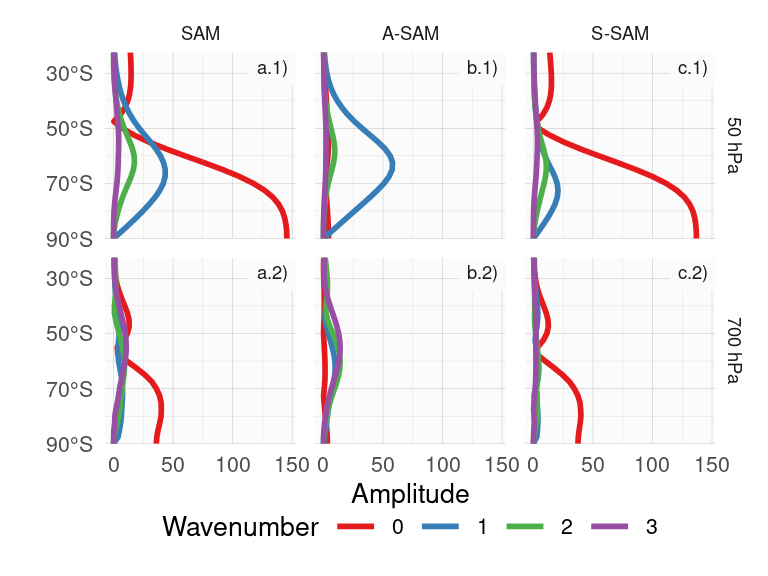
\includegraphics{figures/30-sam/wave-amplitude-1} 

}

\caption{Amplitud (metros) de las ondas zonales de los patrones de regresión de altura geopotencial de la Figura \ref{fig:2d-regr} para ondas zonales con número de onda 0, 1, 2 y 3, donde el número de onda 0 representa la amplitud de la media zonal.}\label{fig:wave-amplitude}
\end{figure}

La amplitud de las ondas zonales con números de onda 0 a 3 en cada latitud a 50 hPa y 700 hPa se muestran en la Figura \ref{fig:wave-amplitude}, donde el número de onda cero representa la amplitud de la media zonal.
Las amplitudes de las ondas zonales del patrón espacial descrito por el índice SAM (Fig. \ref{fig:wave-amplitude} columna a) están dominadas por la media zonal (número de onda 0) en ambos niveles.
Sin embargo, las ondas zonales son importantes, sobre todo al sur de 50ºS, con un número de onda 1 claramente dominante en 50 hPa (Fig. \ref{fig:wave-amplitude}a.1) y una mezcla de ondas de amplitud similar en 700 hPa (Fig. \ref{fig:wave-amplitude}a.2).
La Figura \ref{fig:wave-amplitude} columna b muestra que el A-SAM está dominado principalmente por la onda 1 en la estratosfera (Fig. \ref{fig:wave-amplitude}b.1), mientras que en la troposfera se explica por una combinación de ondas zonales 3 a 1 en nivel decreciente de importancia (Fig. \ref{fig:wave-amplitude}b.2) con una amplitud despreciable de la media zonal.
Por otra parte, el S-SAM se explica casi en su totalidad por la media zonal en ambos niveles (Fig. \ref{fig:wave-amplitude} columna c), con poca o ninguna contribución de las ondas zonales con números de onda de 1 a 3.



\begin{figure}

{\centering 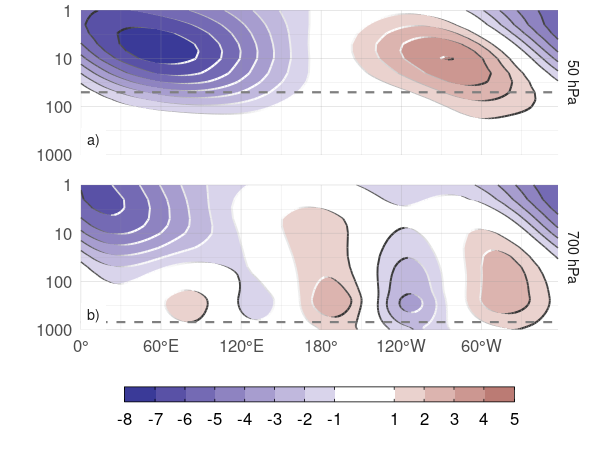
\includegraphics{figures/30-sam/vertical-regression-1} 

}

\caption{Regresión de las anomalías mensuales de altura geopotencial promediada entre 65ºS y 45ºS (metros) y el índice A-SAM de 50 hPa (a) y 700 hPa (b) (niveles indicados en línea punteada) para el período 1979--2020.}\label{fig:vertical-regression}
\end{figure}

Para analizar la estructura vertical de las anomalías de altura geopotencial asociadas al índice A-SAM, mostramos una sección transversal vertical de regresiones de anomalías de altura geopotencial promediadas entre 65ºS y 40ºS con el índice A-SAM de 50 hPa (Fig. \ref{fig:vertical-regression}a) y con el índice A-SAM de 700 hPa (Fig. \ref{fig:vertical-regression}b).
Las anomalías de altura geopotencial asociadas a el A-SAM estratosférico (Fig. \ref{fig:vertical-regression}a) están claramente limitadas a la estratosfera, lo que subraya el desacoplamiento entre el A-SAM estratosférico y el troposférico.
La estructura vertical de esta señal se inclina unos 60 grados hacia el oeste entre 100 hPa y 1 hPa, lo que sugiere procesos baroclínicos.
La señal en la estratosfera se maximiza cerca de 10 hPa a pesar de utilizar el índice de 50 hPa para la regresión.

El A-SAM troposférico (Fig. \ref{fig:vertical-regression}b) presenta señales significativas que se extienden hacia arriba hasta los niveles más altos del reanálisis.
En la troposfera, la estructura de la onda 3 es barotrópica equivalente, con una amplitud máxima en torno a los 250 hPa.
Las anomalías son mayores en el hemisferio occidental, donde se extienden hasta la estratosfera.
En el hemisferio oriental, la señal de la onda 3 es menor y se limita a la troposfera, mientras que las anomalías negativas dominan en la estratosfera.
Aunque el índice A-SAM troposférico está asociado a anomalías geopotenciales estratosféricas, éstas no se proyectan fuertemente sobre el A-SAM estratosférico.
Las estructuras mostradas en la Figura \ref{fig:vertical-regression} son robustas a la elección del nivel del índice.
Para cualquier índice estratosférico (por encima de 100 hPa), las anomalías resultantes son muy similares a la estructura de onda-1 con máximo cerca de 10 hPa en la Figura \ref{fig:vertical-regression}a.
Por el contrario, para cualquier índice troposférico (por debajo de 100 hPa), el resultado es muy similar al de la Figura \ref{fig:vertical-regression}b.
Los patrones cambian principalmente en amplitud (no se muestra).



\begin{table}

\caption{\label{tab:enso-cor-table}Correlación entere los índices del SAM y el ONI. En negrita, las correlaciones con p-valor ajustado por FDR menores a 0.01.}
\centering
\begin{tabular}[t]{c>{}c>{}c>{}c}
\toprule
\multicolumn{1}{c}{ } & \multicolumn{1}{c}{Correlación} & \multicolumn{2}{c}{Correlación parcial} \\
\cmidrule(l{3pt}r{3pt}){2-2} \cmidrule(l{3pt}r{3pt}){3-4}
 & SAM & A-SAM & S-SAM\\
\midrule
 & \textbf{-0.17} & \textbf{-0.25} & 0.00\\
\cmidrule{2-4}
\multirow[t]{-2}{*}{\centering\arraybackslash Year} & \textbf{(<0.001)} & \textbf{(<0.001)} & (0.993)\\
\cmidrule{1-4}
 & \textbf{-0.32} & \textbf{-0.31} & -0.19\\
\cmidrule{2-4}
\multirow[t]{-2}{*}{\centering\arraybackslash DJF} & \textbf{(<0.001)} & \textbf{(0.002)} & (0.068)\\
\cmidrule{1-4}
 & -0.05 & \textbf{-0.25} & 0.15\\
\cmidrule{2-4}
\multirow[t]{-2}{*}{\centering\arraybackslash MAM} & (0.678) & \textbf{(0.009)} & (0.156)\\
\cmidrule{1-4}
 & 0.02 & -0.13 & 0.11\\
\cmidrule{2-4}
\multirow[t]{-2}{*}{\centering\arraybackslash JJA} & (0.948) & (0.218) & (0.300)\\
\cmidrule{1-4}
 & \textbf{-0.26} & \textbf{-0.40} & 0.00\\
\cmidrule{2-4}
\multirow[t]{-2}{*}{\centering\arraybackslash SON} & \textbf{(0.008)} & \textbf{(<0.001)} & (0.993)\\
\bottomrule
\end{tabular}
\end{table}

El patrón de la onda 3 de la Figura \ref{fig:2d-regr}b.2 es muy similar al PSA (Mo y Ghil 1987; Kidson 1988), que es un patrón de teleconexión asociado al ENSO (Karoly 1989).
De hecho, Fogt, Bromwich y Hines (2011) demostró que existe una relación significativa entre el SAM y el ENSO.
La correlación entre el SAM y el ENSO (medido por el Índice del Niño Oceánico (ONI, Bamston, Chelliah y Goldenberg 1997)) se muestra en la Tabla \ref{tab:enso-cor-table} para cada índice SAM y para cada trimestre y para todo el año.
Existe una correlación significativa entre SAM y ENSO que, cuando se divide en trimestres, sólo es es importante en DJF y SON.
Esta relación es captada principalmente por el A-SAM, ya que este índice presenta correlaciones parciales significativas con el ENSO, mientras que las correlaciones con el S-SAM son todas menores y no significativas.
Incluso en los trimestres donde la correlación entre SAM y ENSO es esencialmente nula (MAM y JJA), la correlación parcial entre el A-SAM es mucho más alta; en MAM incluso es significativa al nivel del 95\%.
El mismo análisis se realizó utilizando el Índice ENSO Multivariado (Wolter y Timlin 2011) y el Índice de Oscilación del Sur (Ropelewski y Jones 1987), obteniendo resultados similares.
Esto último nos permite concluir que estos resultados no dependen del índice ENSO utilizado.

\hypertarget{impacts}{%
\section{Impactos}\label{impacts}}



\begin{figure}

{\centering 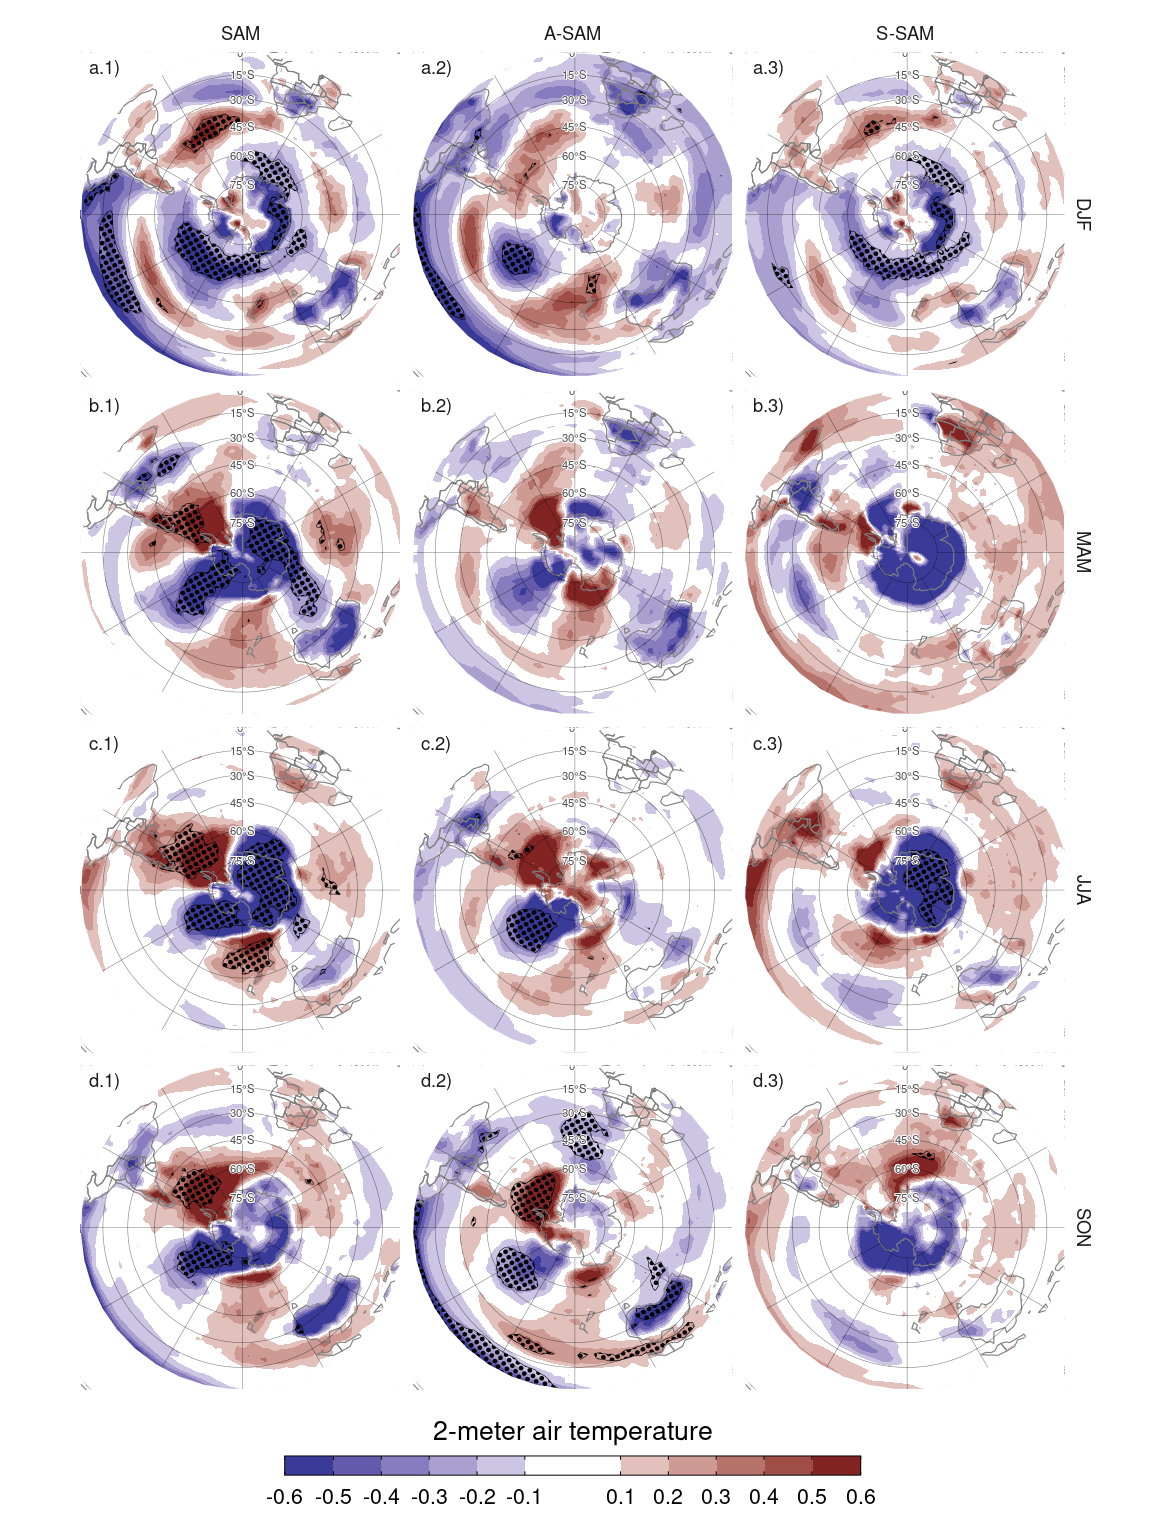
\includegraphics{figures/30-sam/regr-air-season-1} 

}

\caption{Regresión de las anomalías de temperatura a dos metros (Kelvin) con el índice SAM (columna a), A-SAM (columna b) y S-SAM (columna c) en cada trimestre para el período 1979--2020. Áreas con puntos marcan regiones donde el p-valor es menor que 0.01 ajustado por FDR. La escala de colores se corta en \(\pm0.6 \mathrm{K}\) para resaltar valores de regresión en los trópicos y latitudes medias a expensas de los valores en las regiones polares.}\label{fig:regr-air-season}
\end{figure}

Para evaluar las diferencias en los impactos asociados a los índices SAM, A-SAM y S-SAM, realizamos una regresión de la temperatura del aire y la precipitación a 2 metros sobre cada uno de los tres índices del SAM de 700 hPa.
Como se mostró en secciones anteriores, los tres índices son muy coherentes en la troposfera, por lo que seleccionamos este nivel para representar la circulación troposférica por compatibilidad con la literatura previa.
Las regresiones se realizaron sin quitarle la tendencia ni a las variables ni a los índices, pero calcular las regresiones con valores sin tendencias no cambia los resultados considerablemente (no se muestra).

La Figura \ref{fig:regr-air-season} muestra las regresiones con la temperatura a 2 metros.
En verano, los valores positivos del índice SAM (Fig. \ref{fig:regr-air-season}a.1) se asocian a anomalías negativas de temperatura cerca de la Antártida rodeadas por un anillo de anomalías positivas en las latitudes medias.
El anillo no es zonalmente simétrico, ya que hay cuatro máximos locales distintivos en torno a 30ºW, 120ºW, 150ºE y 90ºE respectivamente.
En los trópicos, las anomalías son negativas en el Pacífico ecuatorial, lo que concuerda con la correlación negativa entre SAM y ENSO observada en la Tabla \ref{tab:enso-cor-table}.
Los paneles a.2 y a.3 de la Figura \ref{fig:regr-air-season} muestran que tanto las anomalías zonales de este patrón como los altos valores en los trópcios están asociados principalmente al A-SAM y que el S-SAM está asociado a anomalías de temperatura más zonalmente simétricas en latitudes altas.
Sobre la Antártida, los valores positivos del índice SAM están asociados a anomalías negativas de temperatura, en particular sobre la costa oriental.
Estas anomalías están asociadas únicamente con el S-SAM.
Por otro lado, las anomalías de temperatura en el océano Índico, el sur de África y Australia están fuertemente relacionadas con A-SAM y no están presentes en el patrón de regresión con el SAM.

En otoño, invierno y primavera (filas b, c y d en la Figura \ref{fig:regr-air-season}) el SAM está asociado a un patrón de anomalías de temperatura zonalmente asimétrico en latitudes altas, con valores negativos sobre la Antártida y el Mar de Amundsen y positivas al sur de Nueva Zelanda y centradas en el pasaje de Drake que se extienden hasta la Patagonia.
Esto refleja la naturaleza más asimétrica del SAM durante estas estaciones en comparación al verano.
Jones et~al. (2019) observó características similares en las mediciones de estaciones, aunque utilizando datos de 1957 a 2016.
En general se observa que la señal sobre la Antártida está asociada al S-SAM (aunque estadísticamente significativa sólo en invierno), mientras que las anomalías sobre el Océano Antártico y latitudes más bajas se asocian al A-SAM.
En primavera, la señal tropical de A-SAM es similar a la del verano, revelando de nuevo la importancia del vínculo ENSO-\/-A-SAM.

El patrón de anomalías negativas en el polo rodeadas de anomalías positivas que se observa aproximadamente en todas las estaciones -aunque con intensidad variable y detalles a pequeña escala- se traduce en un gradiente de temperatura meridional aumentado maximizado en la línea cero, lo que es coherente con la intensificación y migración hacia el polo de los vientos del oeste comúnmente vinculados a el SAM a través del balance térmico del viento.
Por tanto, no es sorprendente verlo más claramente asociado al S-SAM.
Las temperaturas sobre la Antártida Oriental se ven más afectadas por el S-SAM, mientras que en la Antártida Occidental son más sensibles al A-SAM.
Dado que el índice S-SAM está negativamente correlacionado con la temperatura sobre la Antártida Oriental, es posible que la tendencia positiva en el índice S-SAM pueda ayudar a explicar la falta de tendencia positiva de la temperatura en la Antártida Oriental en comparación con la Antártida Occidental en el contexto del calentamiento global (Nicolas y Bromwich 2014).



\begin{figure}

{\centering 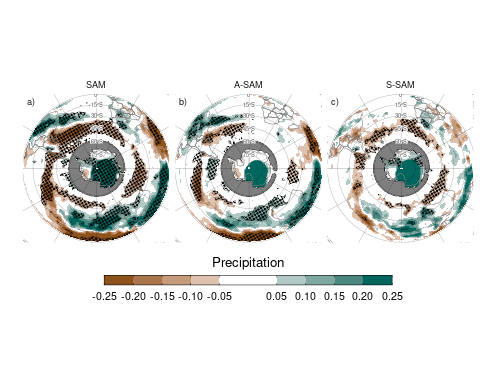
\includegraphics{figures/30-sam/global-pp-1} 

}

\caption{Regresión de anomalías de precipitación (mm por día) con el SAM (a), A-SAM (b) y S-SAM (c) para el período 1979--2020. En gris, las zonas con valores faltantes. Áreas con puntos marcan regiones donde el p-valor es menor que 0.01 ajustado por FDR. La escala de colores se corta en \(\pm0.25 \mathrm{K}\) para resaltar valores de regresión en los trópicos y latitudes medias a expensas de los valores en las regiones polares.}\label{fig:global-pp}
\end{figure}

La Figura \ref{fig:global-pp} muestra la regresión de los índices SAM con la precipitación para el hemisferio sur.
La señal de precipitación asociada a SAM (Fig. \ref{fig:global-pp}a) muestra en general una disminución de la precipitación en torno a los 45ºS, un ligero aumento de la precipitación en torno a los 30ºS y un aumento de la precipitación sobre la Antártida, un patrón descrito por otros estudios (p.~ej. Hendon, Lim y Nguyen 2014).
Este patrón se mantiene prácticamente sin cambios entre estaciones, aunque varía en intensidad (no se muestra).
Los paneles b y c de la Figura \ref{fig:global-pp} muestran que la señal A-SAM sólo se da en los trópicos y latitudes medias, mientras que la señal S-SAM es fuerte en las latitudes altas.
En particular, los valores positivos de S-SAM se asocian con el aumento de las precipitaciones sobre la Antártida y la disminución de las precipitaciones alrededor del Océano Austral.

Para estudiar con más detalle los impactos locales, las Figuras \ref{fig:pp-regr-oceania} y \ref{fig:pp-regr-america} muestran la regresión de los índices SAM con la precipitación media estacional y la altura geopotencial de 700 hPa para Nueva Zelanda e islas aledañas, y Sudamérica respectivamente.
No se muestra Sudáfrica porque allí no se detectó ninguna señal significativa.



\begin{figure}

{\centering 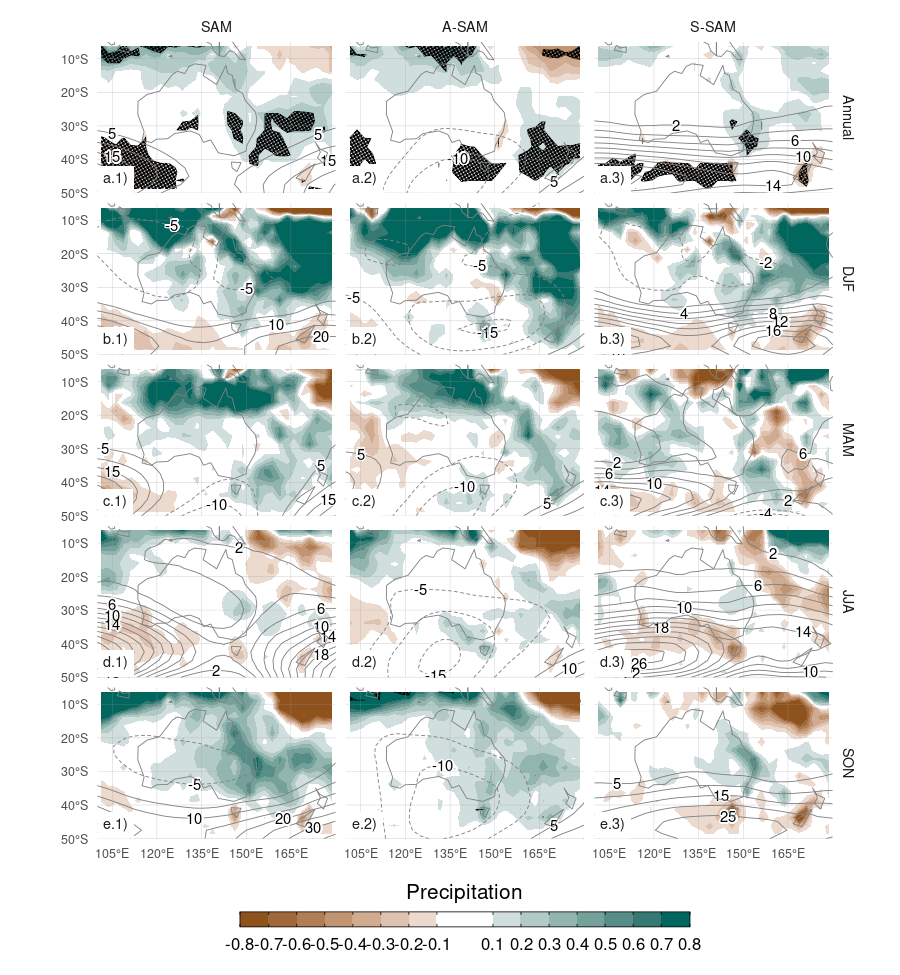
\includegraphics{figures/30-sam/pp-regr-oceania-1} 

}

\caption{Regresión de anomalías de precipitación (mm por día, sombrado) y anomalías de altura geopotencial (líneas finas, valores positivos en líneas llenas y negativos en líneas punteadas) para todo el año (fila a) y medias estacionales (filas b a e) con el SAM (columna 1), A-SAM (columna 2) y S-SAM (columna 3) para el período 1979--2020. Nueva Zelanda e islas aledañas. Áreas con puntos marcan regiones donde el p-valor es menor que 0.01 ajustado por FDR.}\label{fig:pp-regr-oceania}
\end{figure}

En Australia, la regresión anual muestra que el índice SAM está asociado con anomalías positivas de precipitación en la región sudeste (Fig. \ref{fig:pp-regr-oceania}a.1), en acuerdo con Gillett, Kell y Jones (2006).
La separación entre A-SAM y S-SAM sugiere que esta anomalía positiva se explica por el S-SAM sólo en la costa este (Fig. \ref{fig:pp-regr-oceania}c.1).
Las anomalías de altura geopotencial asociadas a este índice (contornos negros) son indicativas de un flujo hacia el este procedente del mar de Tasmania, lo que podría explicar las anomalías positivas en las precipitaciones encontradas por Hendon, Thompson y Wheeler (2007).
El A-SAM parece estar relacionado con anomalías positivas de precipitación en la costa oeste del sureste de Australia (Fig. \ref{fig:pp-regr-oceania}b.2), que podrían explicarse de forma similar por la circulación anómala del oeste que transporta aire húmedo al continente desde el océano Índico.

Las regresiones estacionales muestran anomalías estadísticamente significativas sólo en primavera, cuando un SAM positivo se asocia con anomalías positivas de precipitación en el este y centro de Australia (Fig. \ref{fig:pp-regr-oceania}a.5).
En este trimestre, el S-SAM parece estar asociado con anomalías positivas de precipitación en un área relativamente reducida de la costa oriental (Fig. \ref{fig:pp-regr-oceania}c.5) mientras que las anomalías positivas de precipitación relacionadas con A-SAM positivo afectan a todo el este de Australia (Fig. \ref{fig:pp-regr-oceania}b.5).

En verano, un índice SAM positivo se asocia con anomalías de precipitación positivas en Australia occidental y oriental, sobre todo en la región noreste (Fig. \ref{fig:pp-regr-oceania}a.2).
La parte oriental está dominada por la relación con el S-SAM y la occidental, por el A-SAM.
En otoño, la regresión con el SAM muestra anomalías positivas en el norte, similares a las de verano, que se asocian con el A-SAM.
En invierno los coeficientes de regresión son mucho más débiles que durante el resto del año.
Ninguno de estos coeficientes de regresión es estadísticamente significativo al nivel del 95\%.
La señal de la primavera coincide en líneas generales con Hendon, Thompson y Wheeler (2007), pero mientras que ellos también detectaron una fuerte señal en verano, la Figura \ref{fig:pp-regr-oceania}a.2 no muestra ninguna asociación estadísticamente significativa (aunque los coeficientes tienen un signo coherente).



\begin{figure}

{\centering 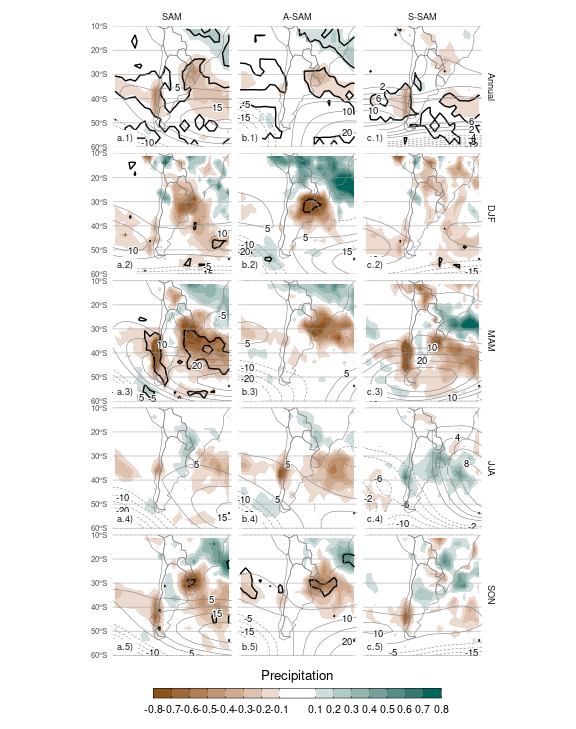
\includegraphics{figures/30-sam/pp-regr-america-1} 

}

\caption{Igual que la Figura \ref{fig:pp-regr-oceania} pero para Sudamérica.}\label{fig:pp-regr-america}
\end{figure}

En Sudamérica (Fig. \ref{fig:pp-regr-america}), la regresión anual muestra que el SAM positivo está asociado a anomalías de precipitación negativas en el Sudeste de Sudamérica (SESA) y el sur de Chile, y anomalías positivas en el sur de Brasil, cerca de la Zona de Convergencia del Atlántico Sur (SACZ) (Fig. \ref{fig:pp-regr-america}a.1).
Las figuras \ref{fig:pp-regr-america}b.1 y c.1 muestran que mientras la señal sobre SESA y el sur de Brasil está asociada con A-SAM, la del sur de Chile está relacionada con S-SAM.

Excepto en invierno, las regresiones estacionales reflejan este mismo patrón.
Aunque no sean estadísticamente significativas, todas muestran valores negativos en SESA y el sur de Chile junto con valores positivos en el sur de Brasil en relación con el SAM.
La separación de estas características entre los mapas de regresión A-SAM y S-SAM es también bastante consistente.

La circulación anómala a 700 hPa asociada a S-SAM (Fig. \ref{fig:pp-regr-america}c.1) indica un flujo anómalo del este sobre el sur de Chile.
Esto conduce a una menor advección de aire húmedo desde el Océano Pacífico, que es la principal fuente de agua precipitable en esa región (Garreaud 2007).
Por otro lado, la circulación anómala asociada a valores positivos del A-SAM (Fig. \ref{fig:pp-regr-america}b.1) en el Atlántico es anticiclónica al este y ciclónica al oeste de Sudamérica.
Esto promueve un flujo anómalo del sudeste sobre el SESA que inhibe el flujo del chorro de baja altura desde Sudamérica hacia la región (Silvestri y Vera 2009; Zamboni, Mechoso y Kucharski 2010).
Se encontró que este mismo patrón está asociado con el aumento de las precipitaciones en el sur de Brasil durante los eventos de SACZ (Rosso et~al. 2018).
Hay una pequeña área de anomalías positivas significativas de precipitación con el SAM cerca del centro de Argentina, también observado en el análisis basado en estaciones de Gillett, Kell y Jones (2006), que se explica por el A-SAM.

\hypertarget{conclusiones-1}{%
\section{Conclusiones}\label{conclusiones-1}}

La división del SAM entre su parte zonalmente asimétrica y simétrica muestra que estos dos aspectos del SAM tienen variabilidad, tendencias e impactos distintivos.

En el capítulo siguiente estudiará la relación entre los cEOFs y las distintas componentes del SAM.

\hypertarget{sam-ceof}{%
\chapter{Relación entre los modos de variabilidad del hemisferio sur}\label{sam-ceof}}

En los capítulos anteriores se describieron los modos de circulación del hemisferio sur a través de Funciones Empíricas Complejas (cEOF) y las componentes simétricas y asimétricas del Modo Anular del Sur (SAM).
En este capítulo se explora la relación entre estos modos de variabilidad, así como con el Modo del Pacífico-Sudamérica (PSA).
Éste último se calcula según Mo y Paegle (2001) como el segundo y tercer EOF de las anomalías trimestrales de altura geopotencial en 500 hPa.

\hypertarget{sam}{%
\section{SAM}\label{sam}}




\begin{figure}

{\centering 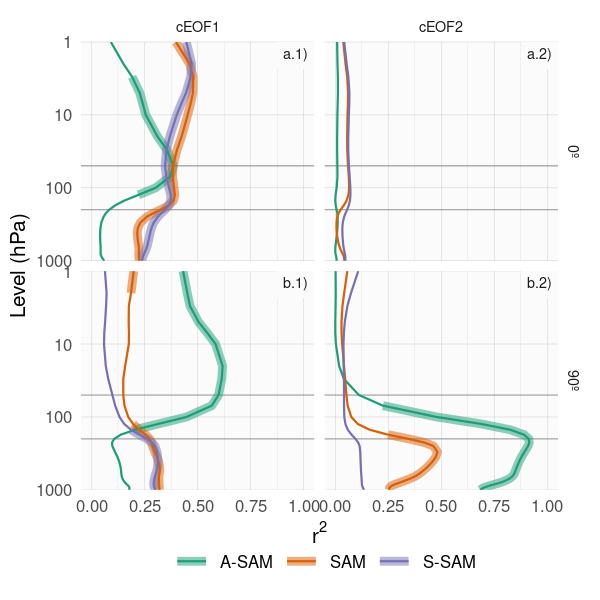
\includegraphics{figures/40-sam-ceof/sam-eof-vertical-1} 

}

\caption{Coeficiente de determinación (\(r^2\)) entre la fase de 0º (fila a) y 90º (fila b) de los cEOFs con el SAM, A-SAM y S-SAM para cada nivel durante el período 1979--2020.
Las líneas gruesas representan valores con p-valor menor a 0.01 ajustado por FDR.}\label{fig:sam-eof-vertical}
\end{figure}

Calculamos el coeficiente de determinación entre las series temporales de los cEOFs y los tres índices SAM (SAM, A-SAM y S-SAM) definidos en cada nivel vertical (Fig.~\ref{fig:sam-eof-vertical}).
El índice SAM está correlacionado de forma estadísticamente significativa con la fase de 0º del cEOF1 en todos los niveles, y con la fase de 90º del cEOF1 y la fase de 90º del cEOF2 en la tropósfera.
Por otro lado, las correlaciones entre SAM y la fase de 0º del cEOF2 son prácticamente nulas.

En la tropósfera la correlación de ambas fases del cEOF1 y el SAM es igual a su correlación con el S-SAM, y su correlación con el A-SAM es mucho más baja y no significativa.
Esto indica que la relación entre el SAM y el cEOF1 en la tropósfera se explica en su totalidad por la componente zonalmente simétrica del SAM.
En la estratosfera, la fase de 0º del cEOF1 está correlacionada tanto con la A-SAM como con la S-SAM, mientras que la fase de 90º está altamente correlacionada sólo con la A-SAM.
Estas correlaciones son consistentes con los mapas de regresión de la altura geopotencial en la Figura \ref{fig:eof1-regr-gh} y su comparación con los obtenidos para SAM, A-SAM y S-SAM (Fig. \ref{fig:2d-regr}).

La falta de relación fuerte entre el cEOF1 y la TSM, la temperatura y la precipitación observada en la Sección \ref{fuentes-ceof} podría ser sorprendente teniendo en cuenta la correlación entre el cEOF1 y el SAM (Fig. \ref{fig:sam-eof-vertical} columna 1) y la correlación entre el SAM y la TSM del Pacífico Central, la temperatura al este y oeste de la Península Antártica, y con la precipitación en el oeste de Australia (Fogt y Marshall 2020).
Esto se debe principalmente a dos razones.
En primer lugar, la correlación entre cEOF1 y el SAM en la troposfera es modesta, con menos del 50\% de varianza compartida (Fig. \ref{fig:sam-eof-vertical} columna 1), por lo que no se espera que estos índices sean equivalentes.
En segundo lugar, como se demostró en la Sección \ref{impacts}, la fuerte relación entre el SAM y las TSM del Pacífico y las anomalías de temperatura alrededor de la Península Antártica se debe principalmente a la parte asimétrica de el SAM.
Mientras tanto, el cEOF1 está significativamente correlacionado sólo con la parte simétrica de el SAM (Fig. \ref{fig:sam-eof-vertical} columna 1), que por sí misma no está significativamente correlacionada con las temperaturas superficiales en esa zona.

El cEOF2 sólo tiene relación con el SAM en su fase de 90º, asociada a la parte asimétrica y únicamente en la tropósfera.
La correlación entre ambos índices es muy alta, con valores superiores al 75\% de la varianza compartida en toda la tropósfera y un máximo de 92\% en 225 hPa.
Esta altísima correlación es comparable a la correlación observada entre distintos índices del SAM (Ho, Kiem y Verdon-Kidd (2012)) y sugiere que esta fase es capaz de caracterizar la componente zonalmente asimétrica de el SAM en su totalidad.

\hypertarget{psa}{%
\section{PSA}\label{psa}}





\begin{table}

\caption{\label{tab:psa-eof2}Coeficiente de correlación entre las fases del cEOF2 y los modos PSA1 y PSA2 para el período 1979--2020.
Los intervalos de confianza de 95\% se muestran en paréntesis.
Estimaciones con p-valor menor a 0.01 en negrita.}
\centering
\begin{tabular}[t]{l>{}l>{}l}
\toprule
PC & 0º & 90º\\
\midrule
PSA1 & 0.16 (CI: -0.15 -- 0.44) & \textbf{0.74 (CI: 0.56 -- 0.85)}\\
\cmidrule{1-3}
PSA2 & \textbf{0.77 (CI: 0.62 -- 0.87)} & 0.25 (CI: -0.06 -- 0.51)\\
\bottomrule
\end{tabular}
\end{table}

Dada la similitud entre las estructuras asociadas al cEOF2 (Fig. \ref{fig:eof2-regr-gh}) y los patrones del PSA, estudiamos la relación entre ellos.
La tabla \ref{tab:psa-eof2} muestra las correlaciones entre los dos índices del PSA y las series temporales para las fases de 0º y 90º del cEOF2.
Como se anticipaba visualmente la figura \ref{fig:eof2-regr-gh}, existe una gran correlación positiva entre el PSA1 y la fase de 90º y entre el PSA2 y la fase de 0º cEOF2.
Por otro lado, no existe una relación significativa entre el PSA1 y la fase de 0º ni entre el PSA2 y la fase de 90º cEOF2.
En consecuencia, cEOF2 representa bien tanto la estructura espacial como la evolución temporal de los modos PSA, por lo que es posible establecer una asociación entre sus dos fases y los dos modos del PSA.
Es decir, la elección de fase para cEOF2 que maximiza la relación entre ENSO y la fase de 90º del cEOF2, también maximiza la asociación entre los componentes de cEOF2 y los modos PSA (no mostrado).





\begin{figure}

{\centering 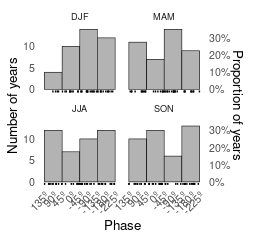
\includegraphics{figures/40-sam-ceof/phase-histogram-1} 

}

\caption{Histograma de la distribución de fases del cEOF2 para el periodo 1979--2020.
Los intervalos están centrados en 90º, 0º, -90º, -180º con un ancho del intervalo de 90º.
Las pequeñas líneas verticales cerca del eje horizontal marcan las observaciones.}\label{fig:phase-histogram}
\end{figure}

La Figura \ref{fig:phase-histogram} muestra un histograma para cada trimestre con la distribución de la fase del cEOF2 con las observaciones marcadas con líneas verticales en el eje horizontal.
En SON (panel 4), el cEOF2 tiene una fase similar a \(\pm\) 90º un 62\% de los años, indicando que es la fase más común.
Esta preferencia de fase está de acuerdo con Irving y Simmonds (2016), que encontró una distribución bimodal a la variabilidad tipo PSA (compare nuestra Figura \ref{fig:phase-histogram} con su Figura 6).

\hypertarget{conclusiuxf3n-1}{%
\section{Conclusión}\label{conclusiuxf3n-1}}

El cEOF2 está íntimamente relacionado con el SAM y el PSA.

En particular, el cEOF2 podría considerarse como una descripción alternativa del PSA, la cual permite caracterizar la amplitud y la fase naturalmente.
En vez de caracterizar al PSA como dos modos estacionarios separados, permite estudiar el continuo de ubicaciones de este modo de variabilidad.

A su vez, la relación entre el cEOF2 y el SAM se explica por que la fase de 90º del cEOF2 describe la variabilidad de la parte asimétrica del SAM en la tropósfera.

Esto sugiere una partición alternativa de la variabilidad de la circulación del hemisferio sur.
En vez de separar al SAM por un lado y al PSA1 y al PSA2 por el otro, se puede separar la variabilidad entre el S-SAM, representando la variabilidad zonalmente simétrica, y el cEOF2, representando variabilidad asimétrica y dónde el A-SAM sería entendido como una fase del cEOF2.

\hypertarget{anuxe1lisis-de-estos-modos-en-los-modelos-de-cmip6}{%
\chapter{Análisis de estos modos en los modelos de CMIP6}\label{anuxe1lisis-de-estos-modos-en-los-modelos-de-cmip6}}

El análisis previo estudió la circulación zonalmente asimétrica en los datos de reanálisis.
Sin embargo, el estudio de tendencias y variabilidad de estos modelos se ve limitada por la corta longitud de los datos observacionales y la posible inhomogeneidad del reanálisis al cambiar la densidad y tipo de observaciones; un problema que afecta particularmente al hemisferio sur.
Además, es imposible abordar la atribución de las tendencias observadas utilizando únicamente observaciones.

Estas limitaciones motivan la inclusión de datos de modelos climáticos.
En este capítulo se analiza la habilidad de los modelos del sexto Proyecto de Intercomparacion de Modelos Acoplados (CMIP6) y del Proyecto de Intercomparación de Modelos de Detección y Atribución (DAMIP) de capturar estos modos y sus principales características.
Al contar con corridas mucho más largas y múltiples miembros por modelo, es posible evaluar las tendencias a largo plazo con mayor robustez.
Utilizando los modelos incluidos en DAMPI, además podemos avanzar en la atribución de las tendencias observadas.

\hypertarget{muxe9todos-4}{%
\section{Métodos}\label{muxe9todos-4}}

\hypertarget{datos-1}{%
\subsection{Datos}\label{datos-1}}

El CMIP6 es un proyecto que organiza numerosos centros de modelado climático para establecer protocolos comunes para realizar experimentos de modelado.
DAMIP es una componente de CMIP6 que cuenta con experimentos particularmente diseñados para realizar estudios de atribución.

\begin{longtable}[]{@{}
  >{\raggedright\arraybackslash}p{(\columnwidth - 10\tabcolsep) * \real{0.6304}}
  >{\raggedleft\arraybackslash}p{(\columnwidth - 10\tabcolsep) * \real{0.0797}}
  >{\raggedleft\arraybackslash}p{(\columnwidth - 10\tabcolsep) * \real{0.0652}}
  >{\raggedleft\arraybackslash}p{(\columnwidth - 10\tabcolsep) * \real{0.0652}}
  >{\raggedleft\arraybackslash}p{(\columnwidth - 10\tabcolsep) * \real{0.0652}}
  >{\raggedleft\arraybackslash}p{(\columnwidth - 10\tabcolsep) * \real{0.0942}}@{}}
\caption{\label{tab:modelos}Modelos analizados y la cantidad de miembros para cada experimento.}\tabularnewline
\toprule()
\begin{minipage}[b]{\linewidth}\raggedright
Modelo
\end{minipage} & \begin{minipage}[b]{\linewidth}\raggedleft
historical
\end{minipage} & \begin{minipage}[b]{\linewidth}\raggedleft
hist-GHG
\end{minipage} & \begin{minipage}[b]{\linewidth}\raggedleft
hist-nat
\end{minipage} & \begin{minipage}[b]{\linewidth}\raggedleft
hist-aer
\end{minipage} & \begin{minipage}[b]{\linewidth}\raggedleft
hist-stratO3
\end{minipage} \\
\midrule()
\endfirsthead
\toprule()
\begin{minipage}[b]{\linewidth}\raggedright
Modelo
\end{minipage} & \begin{minipage}[b]{\linewidth}\raggedleft
historical
\end{minipage} & \begin{minipage}[b]{\linewidth}\raggedleft
hist-GHG
\end{minipage} & \begin{minipage}[b]{\linewidth}\raggedleft
hist-nat
\end{minipage} & \begin{minipage}[b]{\linewidth}\raggedleft
hist-aer
\end{minipage} & \begin{minipage}[b]{\linewidth}\raggedleft
hist-stratO3
\end{minipage} \\
\midrule()
\endhead
AWI-CM-1-1-MR (Semmler et~al. 2018) & 10 & 0 & 0 & 0 & 0 \\
FGOALS-g3 (Li 2019, 2020) & 12 & 3 & 3 & 0 & 0 \\
CanESM5 (Swart et~al. 2019a, 2019b) & 50 & 50 & 50 & 10 & 10 \\
CNRM-CM6-1 (Voldoire 2018, 2019) & 60 & 10 & 10 & 10 & 0 \\
CNRM-ESM2-1 (Seferian 2018) & 21 & 0 & 0 & 0 & 0 \\
ACCESS-ESM1-5 (Ziehn et~al. 2019, 2020) & 80 & 3 & 3 & 0 & 0 \\
ACCESS-CM2 (Dix et~al. 2019, 2020) & 10 & 3 & 3 & 0 & 0 \\
IPSL-CM6A-LR (Boucher, Denvil, Levavasseur, Cozic, Caubel, Foujols, Meurdesoif, Cadule, et~al. 2018; Boucher, Denvil, Levavasseur, Cozic, Caubel, Foujols, Meurdesoif y Gastineau 2018) & 66 & 10 & 10 & 10 & 10 \\
MIROC6 (Tatebe y Watanabe 2018; Shiogama 2019) & 100 & 50 & 50 & 3 & 10 \\
HadGEM3-GC31-LL (Ridley et~al. 2018; Jones 2019) & 10 & 5 & 10 & 4 & 0 \\
UKESM1-0-LL (Tang et~al. 2019; Shim et~al. 2020) & 30 & 0 & 0 & 0 & 0 \\
MPI-ESM1-2-HR (Jungclaus et~al. 2019) & 20 & 0 & 0 & 0 & 0 \\
MPI-ESM1-2-LR (Wieners et~al. 2019) & 60 & 0 & 0 & 0 & 0 \\
GISS-E2-1-G (Space Studies (NASA/GISS) 2018a, 2018b) & 24 & 10 & 20 & 0 & 5 \\
CESM2 (Danabasoglu 2019a, 2019b) & 22 & 3 & 3 & 0 & 0 \\
NorCPM1 (Bethke et~al. 2019) & 60 & 0 & 0 & 0 & 0 \\
NESM3 (Cao y Wang 2019) & 10 & 0 & 0 & 0 & 0 \\
E3SM-1-0 (Bader et~al. 2019; «E3SM-Project E3SM1.0 model output prepared for CMIP6 DAMIP» 2022) & 10 & 3 & 0 & 0 & 0 \\
INM-CM5-0 (Volodin et~al. 2019) & 20 & 0 & 0 & 0 & 0 \\
BCC-CSM2-MR (Xin et~al. 2019) & 0 & 3 & 3 & 3 & 0 \\
MRI-ESM2-0 (Yukimoto et~al. 2019) & 20 & 5 & 5 & 2 & 3 \\
NorESM2-LM (Seland et~al. 2019) & 0 & 3 & 3 & 0 & 0 \\
GFDL-CM4 (Ploshay et~al. 2018) & 0 & 0 & 3 & 0 & 0 \\
GFDL-ESM4 (Horowitz et~al. 2018) & 0 & 1 & 3 & 0 & 0 \\
\bottomrule()
\end{longtable}

Los modelos usados se listan en la Tabla \ref{tab:modelos} se listan todos los modelos y la cantidad de miembros de cada uno.
Usamos todos los modelos de CMIP6 con 5 o más miembros en las corridas históricas (``historical'') y todos los modelos en los experimentos que contienen únicamente el efecto de los gases de efecto invernadero (``hist-GHG''), variabilidad natural sin forzantes antropogénicos (``hist-nat''), forznates de aerosoles antropogénicos (``hist-aer'') o sólo el efecto de el ozono estratosférico (``hist-stratO3'').

Para calcular los cEOFs y evaluar su desempeño, concatenamos todos los miembros para computar un único set de cEOFs para cada modelo y experimento.
Este método trata \(k\) simulaciones de \(n\) años como una única simulación de \(k\times n\) años.
Luego, calculamos los cEOFs siguiendo la metodología de la Sección \ref{ceof-metodo}.
El resultado es que cada modelo y experimento tiene un único patrón espacial (complejo) por cEOF pero una serie temporal (compleja) por miembro.

Para que sea comparable al ERA5, computamos los cEOFs para el período moderno, entre 1979 y 2014 (el último año disponible para todos los miembros).

Como se explicó anteriormente, los cEOFs no están definidos unívocamente ya que aceptan cualquier rotación en el plano complejo análogamente a como los EOFs aceptan cambios de signo.
Los cEOFs computados en ERA5 fueron rotados para maximizar la correlación con el ozono estatosférico o el ENSO como se describe en la Sección \ref{ceof-metodo}.
Para los modelos de CMIP, rotamos los cEOFs para maximizar la correlación espacial de los patrones con el correspondiente cEOF de ERA5.
Esto busca que la localización del patrón sea parecido al observado.

\hypertarget{comparaciuxf3n-con-los-modos-observados}{%
\section{Comparación con los modos observados}\label{comparaciuxf3n-con-los-modos-observados}}

Previo a otros análisis, es encesario evaluar la capacidad de los modelos de capturar las propiedades del los cEOFs observados.
Para esto estudiamos los modelos de las corridas históricas.



\begin{figure}

{\centering 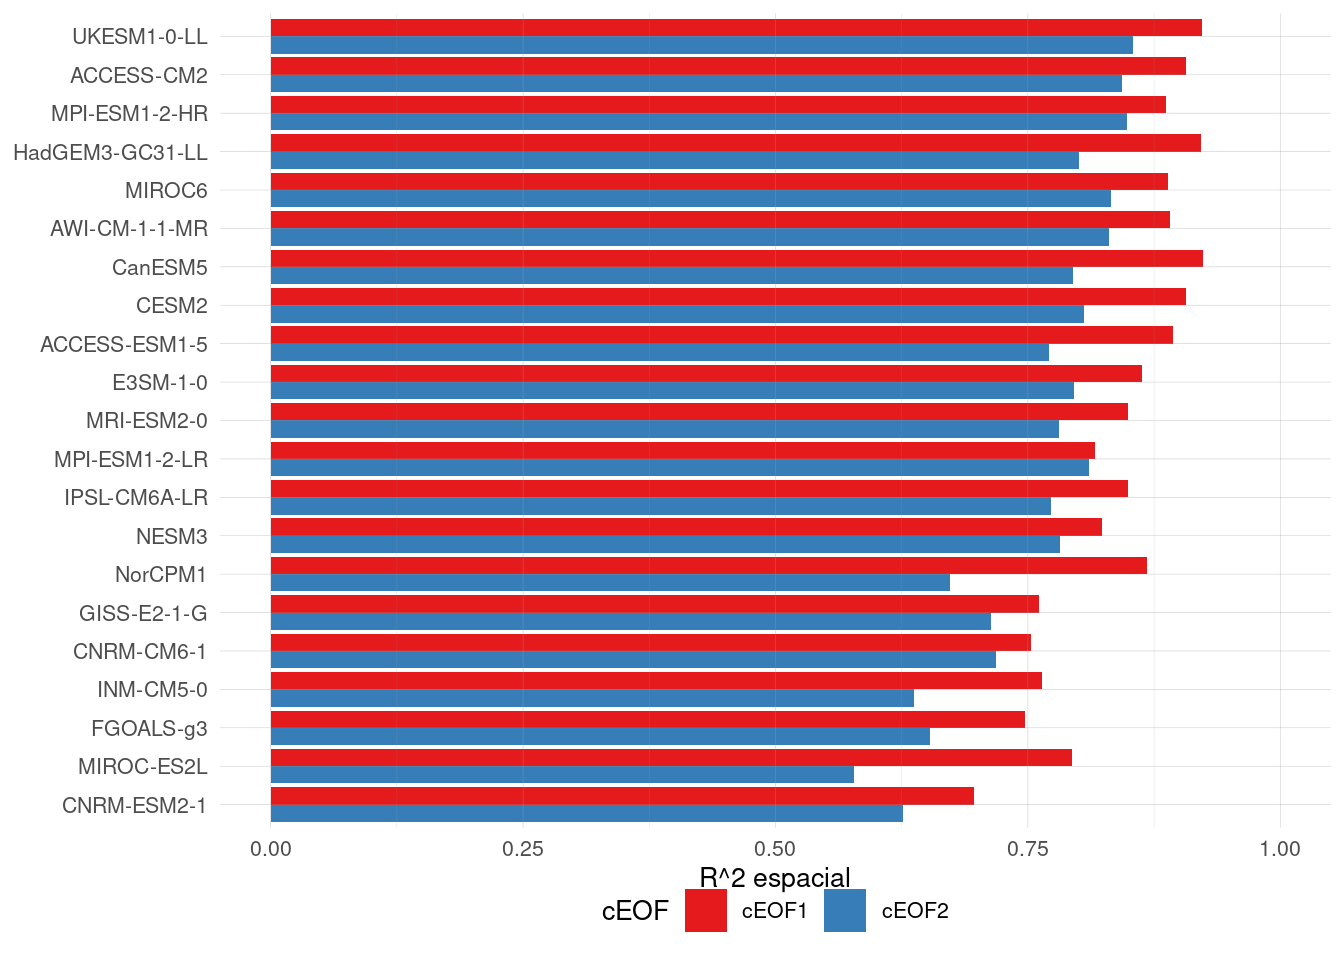
\includegraphics{figures/50-cmip6/comparacion-r2-1} 

}

\caption{\(r^2\) de los patrones espaciales de cada modelo con ERA5 para cada cEOF.}\label{fig:comparacion-r2}
\end{figure}

La Figura~\ref{fig:comparacion-r2} muestra el \(r^2\) de los modelos para los dos cEOFs.
Casi todos los modelos tienen una \(r^2\) mayor a 0,75, indicando que los modelos logran capturar la estructura espacial de los cEOFs correctamente.
Todos los modelos capturan ligeramente mejor el cEOF1 que el cEOF2.

\begin{figure}

{\centering 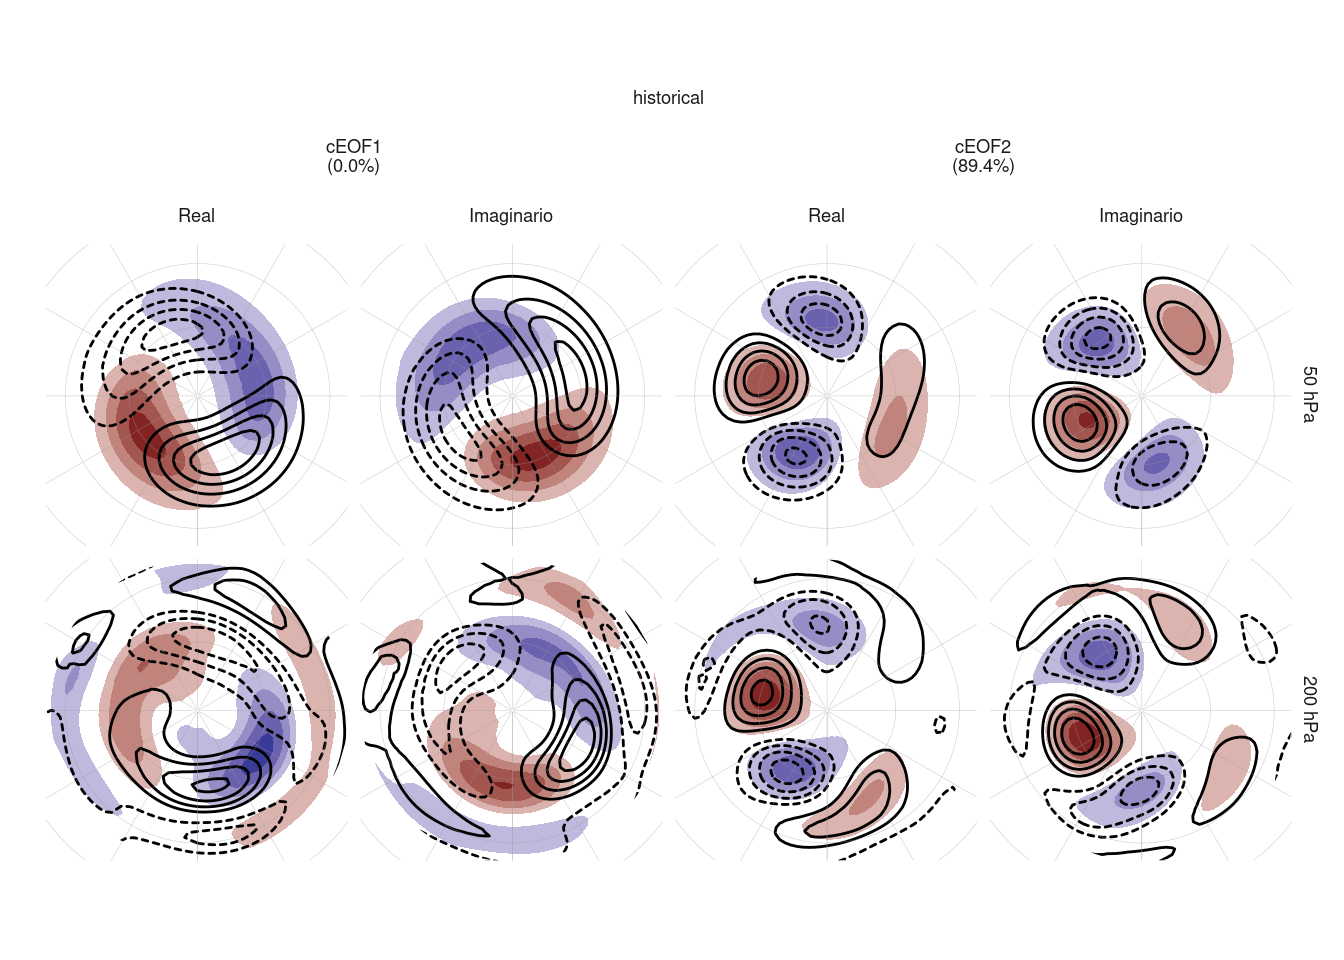
\includegraphics{figures/50-cmip6/mmm-1} 

}

\caption{Media multimodelo (sombreado) de los campos espaciales de cada cEOF, fase y nivel. Los contornos marcan los patrones de ERA5. El \(r^2\) entre ERA5 y la media multimodelo está entre paréntesis.}\label{fig:mmm}
\end{figure}



La Figura \ref{fig:mmm} muestra los patrones promedio multimodelo para cada cEOF y cada fase (es decir, el promedio de los patrones espaciales de cada modelo).
El patrón medio multimodelo es muy similar similar al patrón de ERA5, con niveles de \(r^2\) del orden del 90\%, lo cual lo demuestra que la media multimodelo es más similar a las observaciones que los modelos individuales.

\hypertarget{relaciuxf3n-con-la-variabilidad-tropical}{%
\subsection{Relación con la variabilidad tropical}\label{relaciuxf3n-con-la-variabilidad-tropical}}

\begin{figure}

{\centering 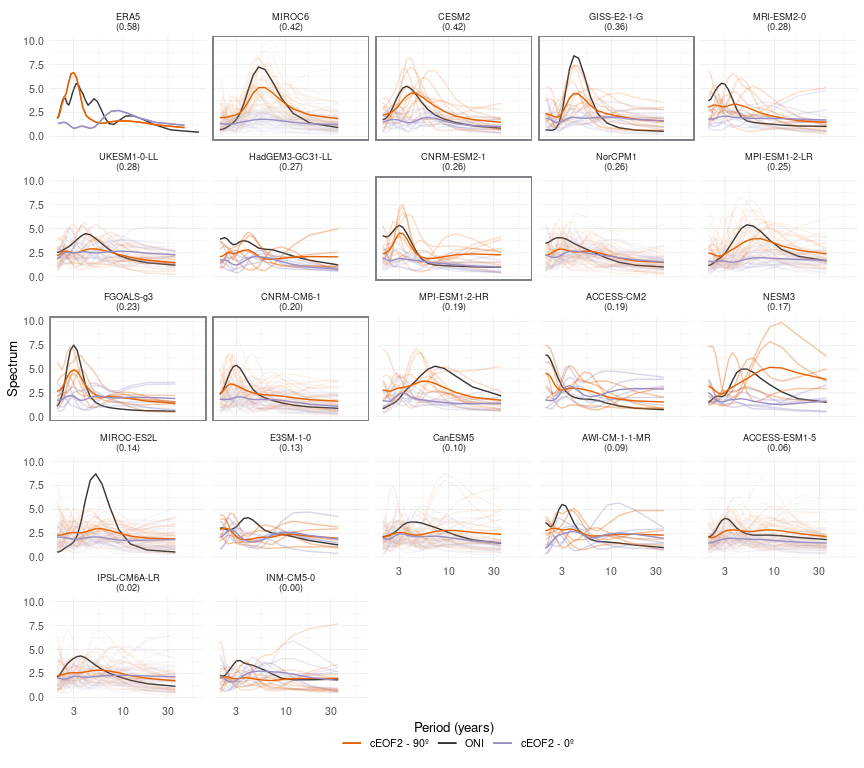
\includegraphics{figures/50-cmip6/fft-ceof2-1} 

}

\caption{Espectros de Fourier para las fases del cEOF2 y del ONI de cada modelo. En línea obscura es el espectro promedio de todos los miembros, que se muestran en líneas translúcidas. El espectro del ONI es el espectro promedio de todos los miembros de cada modelo. Los paneles están ordenados de mayor a menor según el \(r^2\) entre la fase de 90º del cEOF2 y el ONI, el cual se muestra entre paréntesis en el título de cada panel.}\label{fig:fft-ceof2}
\end{figure}





La Figura \ref{fig:fft-ceof2} muestra el periodograma para el cEOF2 con una línea por miembro y una línea gruesa marcando el periodograma promedio, así como el peridiograma promedio del ONI de cada modelo.
La mayoría de los modelos tiene una periodicidad del ONI de \textasciitilde3 años similar a la observada en ERA5, aunque la intensidad y período máximo varía significativamente.

Todos los los modelos que tienen una periodicidad clara en \textasciitilde3 años en la fase de 90º del cEOF2 también tienen una periodicidad del ENSO muy clara y además tienden a tener una correlación entre la fase de 90º del cEOF2 y el ENSO más alta.
Por otro lado, ninguno de los modelos con muy baja correlación con el ENSO pero periodicidad del ENSO clara presenta periocididad clara en el cEOF2.

Sin embargo existen modelos con periodicidad del ENSO clara y correlación relativamente alta que no tienen periodicidad del cEOF2 clara.
MRI-ENSM2-0, UKESM1-0-LL, MPI-ESM1-2-LR son algunos ejemplos.

Estas observaciones sugieren que el ENSO es la fuente de periodicidad del cEOF2 en los modelos de CMIP6 pero que su capacidad para representar la periodicidad observada no sólo depende de la periodicidad del ENSO y del grado de correlación entre los índices.

De todas formas, todos los modelos tienen una correlación entre el ENSO y la fase de 90º del cEOF2 menor a la observada y en muchos de ellos la correlación es prácticamente nula.
Esto indica que si bien los modelos de CMIP6 logran capturar los cEOF, su habilidad para simular la conexión entre éste y el forzante tropical es limitada.



\begin{figure}

{\centering \includegraphics{figures/50-cmip6/sst-mmm-1} 

}

\caption{Media multimodelo de regresión de TSM con los cEOFs. El área sombreada muestra las zonas donde más de la mitad de los modelos tienen p-valor menor a 0.01. Los contornos negros muestran la regresión de TSM observada en ERA5.}\label{fig:sst-mmm}
\end{figure}

Para estudiar más en detalle esa relación, evaluamos la relación entre los cEOF y las anomalías de TSM.
La Figura \ref{fig:sst-mmm} muestra la media multimodelo de la regresión entre TSM y las dos fases de cada cEOF, marcando las zonas donde más de la mitad de los modelos tienen p-valores menores a 0.01.
Los modelos de CMIP6 reproducen los patrones de regresión de la fase de 90º del cEOF2 relativamente bien.
Se observa un exceso de señal en el Pacífico ecuatorial en la fase de 0º del cEOF2 que probablemente se deba a que estos modos no están alineados para minimizar esta relación.
Por otro lado, la señal asociada a la fase de 90º del cEOF1 sí muestra valores excesivamente altos no observados en ERA5.



\begin{figure}

{\centering \includegraphics{figures/50-cmip6/cor-sst-regr-1} 

}

\caption{R\^{}2 entre los patrones de regresión de TSM cada modelo y el patrón de regresión de TSM en ERA5.}\label{fig:cor-sst-regr}
\end{figure}

La Figura \ref{fig:cor-sst-regr} muestra el \(r^2\) los campos de regresión de cada modelo y el campo de regresión de ERA5.
La figura confirma que lo observado para la media multimodelo se cumple para casi todos los modelos individuales.
La mayoría de los modelos tiene un campo de regresión similar a ERA5 para la fase 90º del cEOF2, y una similitud moderada para la fase de 0º.
Para ambas fases del cEOF1, las similitudes son muy bajas.

\begin{figure}

{\centering \includegraphics{figures/50-cmip6/enso-phase-cmip-1} 

}

\caption{Igual que la Figura \ref{fig:enso-phase} pero para los modelos del CMIP6. El ajuste sinusoidal para cada modelo se realiza utilizando todos los miembros.}\label{fig:enso-phase-cmip}
\end{figure}



\begin{figure}

{\centering \includegraphics{figures/50-cmip6/arg-enso-density-1} 

}

\caption{Estimación de densidad por núcleos de la fase del cEOF2 para primaveras con ONI menor a -0.5, entre -0.5 y 0.5, y mayor a 0.5.}\label{fig:arg-enso-density}
\end{figure}



En la Sección \ref{fuentes-ceof} argumentamos que la relación entre el ENSO y el cEOF2 se explica por una preferencia de fase cuando el forzante tropical está activo.
Las Figuras \ref{fig:enso-phase-cmip} muestra la relación entre el ENSO y la fase del cEOF2 para los modelos de CMIP.
Los modelos con una correlación alta entre el cEOF2 y el ENSO muestran una relación sinusoidal similar a la observada en ERA5 con fases cercanas a +90º están asociadas a ONI positivo y viceversa.
La Figura \ref{fig:arg-enso-density} muestra la distribución de fases del cEOF2 para primaveras con ONI menor a -0.5, mayor a 0.5 y valores intermedios.
Cuando el ONI está más activo, el cEOF2 tiene una preferencia de fase de \(\pm90º\), mientras que cuando se encuentra más neutral, la distribución de la fase del cEOF2 es más uniforme.
Esta relación sólo existe en los modelos con mayor relación entre el cEOF2 y el ENSO.
En los modelos con baja correlación, como IPSL-CM6A-LR o INM-CM5-0 la fase del cEOFs es aproximadamente uniforme independientemente del valor del ONI.

\hypertarget{relaciuxf3n-con-el-sam}{%
\subsection{Relación con el SAM}\label{relaciuxf3n-con-el-sam}}

\begin{figure}

{\centering \includegraphics{figures/50-cmip6/cor-sam-cmip6-1} 

}

\caption{Igual que la Figura \ref{fig:sam-eof-vertical} pero para los modelos del CMIP6.}\label{fig:cor-sam-cmip6}
\end{figure}



En la Figura \ref{fig:cor-sam-cmip6} se muestra el \(r^2\) entre las componentes del SAM y las fases de los cEOFs.
Las líneas translúcidas son los valores promedio de cada modelo y las áreas llenas representan el promedio multimodelo y su intervalo de confianza del 95\%; la línea gruesa es el valor de ERA5.

Se observa que la relación entre el SAM y el cEOF2 en los modelos del CMIP6 es prácticamente nula en todos los niveles de la atmósfera, sugiriendo que éstos no capturan esta interacción entre el PSA2 y el SAM.
Sin embargo, sí logran capturar su relación con el A-SAM en la tropósfera; y aunque esta relación tiene menor magnitud en promedio, se observa que ciertos modelos sí consiguen correlaciones comparables con las observadas.

\hypertarget{tendencias}{%
\section{Tendencias}\label{tendencias}}

De la sección anterior surge que los modelos de CMIP6 logran capturar la estructura espacial de los cEOFs así como su variabilidad y relación con otras componentes del sistema climático.
En esta sección, aprovechamos las corridas largas de estos modelos y los experimentos de DAMIP para estudiar las tendencias a largo plazo y sus posibles forzantes.
Para extender las series temporales para todo el período disponible en CMIP6 y DAMIP, proyectamos los campos espaciales del período moderno en los campos desde 1850 hasta 2014.

\begin{figure}

{\centering \includegraphics{figures/50-cmip6/series-largas-1} 

}

\caption{Series temporales de anomalías estandarizadas de los cEOFs computados usando el período 1850 -- 2014. Las anomalías están computadas sobre el período 1850 -- 1900. En líneas translúcidas, las series promedio de cada modelo. En línea oscura, la media multimodelo.}\label{fig:series-largas}
\end{figure}



La Figura \ref{fig:series-largas} muestra las series temporales durante todo el período.
Se observa que la fase de 0º del cEOF1 tiene una tendencia positiva comenzando al rededor de 1950, consistente con la tendencia observada en ERA5 (Fig. \ref{fig:extended-series}).
También se observa una tendencia negativa para la fase de 90º del cEOF1.
Ésta no es detectable en ERA5.
El cEOF2 no presenta tendencias.

\begin{figure}

{\centering \includegraphics{figures/50-cmip6/ceof-damip-1} 

}

\caption{(ref:ceof-damip-cap)}\label{fig:ceof-damip}
\end{figure}

Para tratar de atribuir esta tendencia, computamos los mismos cEOFs para experimentos de DAMIP.
La Figura \ref{fig:ceof-damip} muestra las series temporales para los experimentos hist-GHG, hist-nat, hist-stratO3 e hist-aer junto a las corridas históricas.

Para la fase de 0º del cEOF1, ni hist-nat ni hist-aer mustran tendencias significativas, sugiriendo que la tendencia observada no se debe a variabilidad ni al forzante de los aerosoles antropogénicos.
Por otro lado, hist-stratO3 muestra una tendencia mucho mayor a la observada e hist-GHG muestra una tendencia negativa de similar magnitud la de hist-stratO3.
Esto sugiere que el ozono estatosférico y los gases de efecto invernadero tienen efectos contrarios sobre esta fase del cEOF1.

Una compensación parcial similar también se observa en la fase de 90º del cEOF1, la cual presenta una tendencia negativa en hist-GHG y positiva en hist-aer.



\begin{figure}

{\centering \includegraphics{figures/50-cmip6/suma-1} 

}

\caption{Media multimodelo de las dos fases del cEOF1 para las corridas históricas y para la suma de las corridas hist-GHG, hist-stratO3 e hist-aer.}\label{fig:suma}
\end{figure}

Como una aproximación, la Figura \ref{fig:suma} muestra la media multimodelo de la corrida histórica junto con la suma de las medias multimodelo de las corridas hist-GHG, hist-stratO3 e hist-aer.
Sorpendentemente ambas series presentan una variabilidad a largo plazo virtualmente idéntica, sugiriendo que el efecto de los forzantes es aproximadamente lineal.

\hypertarget{conclusiones-2}{%
\section{Conclusiones}\label{conclusiones-2}}

Los modelos de CMIP6 consiguen caracterizar la estructura espacial de los cEOFs satisfactoriamente, con una buena correlación entre los patrones espaciales, particularmente la media multimodelo.
La habilidad de los modelos de capturar sus características de segundo orden, como la relación con el ENSO y el SAM no es tan buena ni homogénea entre modelos.
Sólo algunos modelos, como MIROC6 y CESM2 consiguen capturar la influencia del ENSO en la fase del cEOF2 y la relación de la mayoría de los modelos con el SAM es menor a la observada.

La tendencia positiva de la fase de 0º del cEOF1 es capturada por la media multimodelo y el análisis de las corridas de DAMIP indican que ésta es forzada principalmente por el forzarte del ozono estratosférico parcialmente compensado por el forzante de los gases de efecto invernadero.
Los modelos de CMIP6 también presentan una tendencia negativa en la fase de 90º del cEOF1 no presente en las observaciones que también es ifluenciada por el forznate antropogénico.

\hypertarget{conclusiones-3}{%
\chapter{Conclusiones}\label{conclusiones-3}}

\backmatter

\hypertarget{referencias}{%
\chapter*{Referencias}\label{referencias}}
\addcontentsline{toc}{chapter}{Referencias}

\markboth{Referencias}{Referencias}

\noindent

\setlength{\parindent}{-0.20in}

\hypertarget{refs}{}
\begin{CSLReferences}{1}{0}
\leavevmode\vadjust pre{\hypertarget{ref-fishpack}{}}%
ADAMS, J.C., SWARTZTRAUBER, P.N. y SWEET, R., 1999. \emph{{FISHPACK}, a Package of {Fortran} Subprograms for the Solution of Separable Elliptic Partial Differential Equations}. 1999. S.l.: https://www2.cisl.ucar.edu/resources/legacy/fishpack.

\leavevmode\vadjust pre{\hypertarget{ref-albers2020}{}}%
ALBERS, S. y CAMPITELLI, E., 2020. \emph{Rsoi: {Import Various Northern} and {Southern Hemisphere Climate Indices}}. agosto 2020. S.l.: s.n.

\leavevmode\vadjust pre{\hypertarget{ref-allaire2020}{}}%
ALLAIRE, J.J., XIE {[}AUT, Y., CRE, MCPHERSON, J., LURASCHI, J., USHEY, K., ATKINS, A., WICKHAM, H., CHENG, J., CHANG, W., IANNONE, R., DUNNING, A., FILTER), A.Y.(Number. sections L., SCHLOERKE, B., DERVIEUX, C., AUST, F., ALLEN, J., SEO, J., BARRETT, M., HYNDMAN, R., LESUR, R., STOREY, R., ARSLAN, R., OLLER, S., RSTUDIO, PBC, LIBRARY), jQuery.F.(jQuery., INST/RMD/H/JQUERY-AUTHORS.TXT), jQuery. contributors (jQuery. library; authors listed in, INST/RMD/H/JQUERYUI-AUTHORS.TXT), jQuery.U. contributors (jQuery.U. library; authors listed in, LIBRARY), M.O.(Bootstrap., LIBRARY), J.T.(Bootstrap., LIBRARY), B. contributors (Bootstrap., TWITTER, LIBRARY), I.(Bootstrap., LIBRARY), A.F.(html5shiv., LIBRARY), S.J.(Respond. js, LIBRARY), I.S.(highlight. js, LIBRARY), G.F.(tocify., TEMPLATES), J.M.(Pandoc., GOOGLE, LIBRARY), I.(ioslides., LIBRARY), D.R.(slidy., LIBRARY), W.(slidy., GANDY (FONT-AWESOME), D., SPERRY (IONICONS), B., (IONICONS), D., STICKYTABS), A.L.(jQuery., FILTER), B.P.J.(pagebreak.L. y FILTER), A.K.(pagebreak.L., 2020. \emph{Rmarkdown: {Dynamic Documents} for {R}}. septiembre 2020. S.l.: s.n.

\leavevmode\vadjust pre{\hypertarget{ref-arblaster2006}{}}%
ARBLASTER, J.M. y MEEHL, G.A., 2006. Contributions of {External Forcings} to {Southern Annular Mode Trends}. \emph{Journal of Climate}, vol. 19, no. 12, ISSN 0894-8755. DOI \href{https://doi.org/10.1175/JCLI3774.1}{10.1175/JCLI3774.1}.

\leavevmode\vadjust pre{\hypertarget{ref-CMIP6.CMIP.E3SM-Project.E3SM-1-0}{}}%
BADER, D.C., LEUNG, R., TAYLOR, M. y MCCOY, R.B., 2019. \emph{E3SM-Project E3SM1.0 model output prepared for CMIP6 CMIP} {[}en línea{]}. 2019. S.l.: Earth System Grid Federation. Disponible en: \url{https://doi.org/10.22033/ESGF/CMIP6.2294}.

\leavevmode\vadjust pre{\hypertarget{ref-baldwin2001}{}}%
BALDWIN, M.P., 2001. Annular Modes in Global Daily Surface Pressure. \emph{Geophysical Research Letters}, vol. 28, no. 21, ISSN 1944-8007. DOI \href{https://doi.org/10.1029/2001GL013564}{10.1029/2001GL013564}.

\leavevmode\vadjust pre{\hypertarget{ref-baldwin2001b}{}}%
BALDWIN, M.P., GRAY, L.J., DUNKERTON, T.J., HAMILTON, K., HAYNES, P.H., RANDEL, W.J., HOLTON, J.R., ALEXANDER, M.J., HIROTA, I., HORINOUCHI, T., JONES, D.B.A., KINNERSLEY, J.S., MARQUARDT, C., SATO, K. y TAKAHASHI, M., 2001. The Quasi-Biennial Oscillation. \emph{Reviews of Geophysics}, vol. 39, no. 2, ISSN 1944-9208. DOI \href{https://doi.org/10.1029/1999RG000073}{10.1029/1999RG000073}.

\leavevmode\vadjust pre{\hypertarget{ref-baldwin2009}{}}%
BALDWIN, M.P. y THOMPSON, D.W.J., 2009. A Critical Comparison of Stratosphere\textendash Troposphere Coupling Indices. \emph{Quarterly Journal of the Royal Meteorological Society}, vol. 135, no. 644, ISSN 1477-870X. DOI \href{https://doi.org/10.1002/qj.479}{10.1002/qj.479}.

\leavevmode\vadjust pre{\hypertarget{ref-bamston1997}{}}%
BAMSTON, A.G., CHELLIAH, M. y GOLDENBERG, S.B., 1997. Documentation of a Highly {ENSO}-related Sst Region in the Equatorial Pacific: {Research} Note. \emph{Atmosphere-Ocean}, vol. 35, no. 3, ISSN 0705-5900. DOI \href{https://doi.org/10.1080/07055900.1997.9649597}{10.1080/07055900.1997.9649597}.

\leavevmode\vadjust pre{\hypertarget{ref-benjamini1995}{}}%
BENJAMINI, Y. y HOCHBERG, Y., 1995. Controlling the {False Discovery Rate}: {A Practical} and {Powerful Approach} to {Multiple Testing}. \emph{Journal of the Royal Statistical Society: Series B (Methodological)}, vol. 57, no. 1, ISSN 2517-6161. DOI \href{https://doi.org/10.1111/j.2517-6161.1995.tb02031.x}{10.1111/j.2517-6161.1995.tb02031.x}.

\leavevmode\vadjust pre{\hypertarget{ref-CMIP6.CMIP.NCC.NorCPM1}{}}%
BETHKE, I., WANG, Y., COUNILLON, F., KIMMRITZ, M., FRANSNER, F., SAMUELSEN, A., LANGEHAUG, H.R., CHIU, P.-G., BENTSEN, M., GUO, C., TJIPUTRA, J., KIRKEVÅG, A., OLIVIÈ, D.J.L., SELAND, ?yvind., FAN, Y., LAWRENCE, P., ELDEVIK, T. y KEENLYSIDE, N., 2019. \emph{NCC NorCPM1 model output prepared for CMIP6 CMIP} {[}en línea{]}. 2019. S.l.: Earth System Grid Federation. Disponible en: \url{https://doi.org/10.22033/ESGF/CMIP6.10843}.

\leavevmode\vadjust pre{\hypertarget{ref-CMIP6.CMIP.IPSL.IPSL-CM6A-LR}{}}%
BOUCHER, O., DENVIL, S., LEVAVASSEUR, G., COZIC, A., CAUBEL, A., FOUJOLS, M.-A., MEURDESOIF, Y., CADULE, P., DEVILLIERS, M., GHATTAS, J., LEBAS, N., LURTON, T., MELLUL, L., MUSAT, I., MIGNOT, J. y CHERUY, F., 2018. \emph{IPSL IPSL-CM6A-LR model output prepared for CMIP6 CMIP} {[}en línea{]}. 2018. S.l.: Earth System Grid Federation. Disponible en: \url{https://doi.org/10.22033/ESGF/CMIP6.1534}.

\leavevmode\vadjust pre{\hypertarget{ref-CMIP6.DAMIP.IPSL.IPSL-CM6A-LR}{}}%
BOUCHER, O., DENVIL, S., LEVAVASSEUR, G., COZIC, A., CAUBEL, A., FOUJOLS, M.-A., MEURDESOIF, Y. y GASTINEAU, G., 2018. \emph{IPSL IPSL-CM6A-LR model output prepared for CMIP6 DAMIP} {[}en línea{]}. 2018. S.l.: Earth System Grid Federation. Disponible en: \url{https://doi.org/10.22033/ESGF/CMIP6.13801}.

\leavevmode\vadjust pre{\hypertarget{ref-cai2020a}{}}%
CAI, W., MCPHADEN, M.J., GRIMM, A.M., RODRIGUES, R.R., TASCHETTO, A.S., GARREAUD, R.D., DEWITTE, B., POVEDA, G., HAM, Y.-G., SANTOSO, A., NG, B., ANDERSON, W., WANG, G., GENG, T., JO, H.-S., MARENGO, J.A., ALVES, L.M., OSMAN, M., LI, S., WU, L., KARAMPERIDOU, C., TAKAHASHI, K. y VERA, C., 2020. Climate Impacts of the {El Niño}\textendash{{Southern Oscillation}} on {South America}. \emph{Nature Reviews Earth \& Environment}, vol. 1, no. 4, ISSN 2662-138X. DOI \href{https://doi.org/10.1038/s43017-020-0040-3}{10.1038/s43017-020-0040-3}.

\leavevmode\vadjust pre{\hypertarget{ref-cai2011}{}}%
CAI, W., RENSCH, P. van, COWAN, T. y HENDON, H.H., 2011. Teleconnection {Pathways} of {ENSO} and the {IOD} and the {Mechanisms} for {Impacts} on {Australian Rainfall}. \emph{Journal of Climate}, vol. 24, no. 15, ISSN 0894-8755, 1520-0442. DOI \href{https://doi.org/10.1175/2011JCLI4129.1}{10.1175/2011JCLI4129.1}.

\leavevmode\vadjust pre{\hypertarget{ref-campitelli2018b}{}}%
CAMPITELLI, E., 2018. {Estudio de los mecanismos físicos asociados con el patrón de onda 3 de la circulación atmosférica del Hemisferio Sur}.,

\leavevmode\vadjust pre{\hypertarget{ref-campitelli2020}{}}%
CAMPITELLI, E., 2020. \emph{{metR}: {Tools} for {Easier Analysis} of {Meteorological Fields}}. abril 2020. S.l.: s.n.

\leavevmode\vadjust pre{\hypertarget{ref-rcmip6}{}}%
CAMPITELLI, E., 2023. \emph{\href{https://doi.org/10.5281/zenodo.10138834}{Rcmip6}}. noviembre 2023. S.l.: Zenodo.

\leavevmode\vadjust pre{\hypertarget{ref-CMIP6.CMIP.NUIST.NESM3}{}}%
CAO, J. y WANG, B., 2019. \emph{NUIST NESMv3 model output prepared for CMIP6 CMIP} {[}en línea{]}. 2019. S.l.: Earth System Grid Federation. Disponible en: \url{https://doi.org/10.22033/ESGF/CMIP6.2021}.

\leavevmode\vadjust pre{\hypertarget{ref-cazes-boezio2003}{}}%
CAZES-BOEZIO, G., ROBERTSON, A.W. y MECHOSO, C.R., 2003. Seasonal {Dependence} of {ENSO Teleconnections} over {South America} and {Relationships} with {Precipitation} in {Uruguay}. \emph{Journal of Climate}, vol. 16, no. 8, ISSN 0894-8755. DOI \href{https://doi.org/10.1175/1520-0442(2003)16\%3C1159:SDOETO\%3E2.0.CO;2}{10.1175/1520-0442(2003)16\textless1159:SDOETO\textgreater2.0.CO;2}.

\leavevmode\vadjust pre{\hypertarget{ref-chung1999}{}}%
CHUNG, C. y NIGAM, S., 1999. Weighting of Geophysical Data in {Principal Component Analysis}. \emph{Journal of Geophysical Research: Atmospheres}, vol. 104, no. D14, ISSN 2156-2202. DOI \href{https://doi.org/10.1029/1999JD900234}{10.1029/1999JD900234}.

\leavevmode\vadjust pre{\hypertarget{ref-clem2013}{}}%
CLEM, K.R. y FOGT, R.L., 2013. Varying Roles of {ENSO} and {SAM} on the {Antarctic Peninsula} Climate in Austral Spring. \emph{Journal of Geophysical Research: Atmospheres}, vol. 118, no. 20, ISSN 2169-8996. DOI \href{https://doi.org/10.1002/jgrd.50860}{10.1002/jgrd.50860}.

\leavevmode\vadjust pre{\hypertarget{ref-CMIP6.CMIP.NCAR.CESM2}{}}%
DANABASOGLU, G., 2019a. \emph{NCAR CESM2 model output prepared for CMIP6 CMIP} {[}en línea{]}. 2019. S.l.: Earth System Grid Federation. Disponible en: \url{https://doi.org/10.22033/ESGF/CMIP6.2185}.

\leavevmode\vadjust pre{\hypertarget{ref-CMIP6.DAMIP.NCAR.CESM2}{}}%
DANABASOGLU, G., 2019b. \emph{NCAR CESM2 model output prepared for CMIP6 DAMIP} {[}en línea{]}. 2019. S.l.: Earth System Grid Federation. Disponible en: \url{https://doi.org/10.22033/ESGF/CMIP6.2187}.

\leavevmode\vadjust pre{\hypertarget{ref-CMIP6.CMIP.CSIRO-ARCCSS.ACCESS-CM2}{}}%
DIX, M., BI, D., DOBROHOTOFF, P., FIEDLER, R., HARMAN, I., LAW, R., MACKALLAH, C., MARSLAND, S., O'FARRELL, S., RASHID, H., SRBINOVSKY, J., SULLIVAN, A., TRENHAM, C., VOHRALIK, P., WATTERSON, I., WILLIAMS, G., WOODHOUSE, M., BODMAN, R., DIAS, F.B., DOMINGUES, C.M., HANNAH, N., HEERDEGEN, A., SAVITA, A., WALES, S., ALLEN, C., DRUKEN, K., EVANS, B., RICHARDS, C., RIDZWAN, S.M., ROBERTS, D., SMILLIE, J., SNOW, K., WARD, M. y YANG, R., 2019. \emph{CSIRO-ARCCSS ACCESS-CM2 model output prepared for CMIP6 CMIP} {[}en línea{]}. 2019. S.l.: Earth System Grid Federation. Disponible en: \url{https://doi.org/10.22033/ESGF/CMIP6.2281}.

\leavevmode\vadjust pre{\hypertarget{ref-CMIP6.DAMIP.CSIRO-ARCCSS.ACCESS-CM2}{}}%
DIX, M., MACKALLAH, C., BI, D., BODMAN, R., MARSLAND, S., RASHID, H., WOODHOUSE, M. y DRUKEN, K., 2020. \emph{CSIRO-ARCCSS ACCESS-CM2 model output prepared for CMIP6 DAMIP} {[}en línea{]}. 2020. S.l.: Earth System Grid Federation. Disponible en: \url{https://doi.org/10.22033/ESGF/CMIP6.14361}.

\leavevmode\vadjust pre{\hypertarget{ref-dowle2020}{}}%
DOWLE, M. y SRINIVASAN, A., 2020. \emph{Data.Table: {Extension} of 'Data.Frame'}. julio 2020. S.l.: s.n.

\leavevmode\vadjust pre{\hypertarget{ref-CMIP6.DAMIP.E3SM-Project.E3SM-1-0}{}}%
\emph{E3SM-Project E3SM1.0 model output prepared for CMIP6 DAMIP} {[}en línea{]}, 2022. 2022. S.l.: Earth System Grid Federation. Disponible en: \url{http://cera-www.dkrz.de/WDCC/meta/CMIP6/CMIP6.DAMIP.E3SM-Project.E3SM-1-0}.

\leavevmode\vadjust pre{\hypertarget{ref-fan2007}{}}%
FAN, K., 2007. Zonal Asymmetry of the {Antarctic Oscillation}. \emph{Geophysical Research Letters}, vol. 34, no. 2, ISSN 0094-8276. DOI \href{https://doi.org/10.1029/2006GL028045}{10.1029/2006GL028045}.

\leavevmode\vadjust pre{\hypertarget{ref-fogt2011a}{}}%
FOGT, R.L., BROMWICH, D.H. y HINES, K.M., 2011. Understanding the {SAM} Influence on the {South Pacific ENSO} Teleconnection. \emph{Climate Dynamics}, vol. 36, no. 7, ISSN 1432-0894. DOI \href{https://doi.org/10.1007/s00382-010-0905-0}{10.1007/s00382-010-0905-0}.

\leavevmode\vadjust pre{\hypertarget{ref-fogt2012}{}}%
FOGT, R.L., JONES, J.M. y RENWICK, J., 2012. Seasonal {Zonal Asymmetries} in the {Southern Annular Mode} and {Their Impact} on {Regional Temperature Anomalies}. \emph{Journal of Climate}, vol. 25, no. 18, ISSN 0894-8755. DOI \href{https://doi.org/10.1175/JCLI-D-11-00474.1}{10.1175/JCLI-D-11-00474.1}.

\leavevmode\vadjust pre{\hypertarget{ref-fogt2020}{}}%
FOGT, R.L. y MARSHALL, G.J., 2020. The {Southern Annular Mode}: {Variability}, Trends, and Climate Impacts across the {Southern Hemisphere}. \emph{WIREs Climate Change}, vol. 11, no. 4, ISSN 1757-7799. DOI \href{https://doi.org/10.1002/wcc.652}{10.1002/wcc.652}.

\leavevmode\vadjust pre{\hypertarget{ref-garreaud2007}{}}%
GARREAUD, R., 2007. Precipitation and {Circulation Covariability} in the {Extratropics}. \emph{Journal of Climate}, vol. 20, no. 18, ISSN 0894-8755. DOI \href{https://doi.org/10.1175/JCLI4257.1}{10.1175/JCLI4257.1}.

\leavevmode\vadjust pre{\hypertarget{ref-gelbrecht2018}{}}%
GELBRECHT, M., BOERS, N. y KURTHS, J., 2018. Phase Coherence between Precipitation in {South America} and {Rossby} Waves. \emph{Science Advances}, vol. 4, no. 12, DOI \href{https://doi.org/10.1126/sciadv.aau3191}{10.1126/sciadv.aau3191}.

\leavevmode\vadjust pre{\hypertarget{ref-gillett2005}{}}%
GILLETT, N.P., ALLAN, R.J. y ANSELL, T.J., 2005. Detection of External Influence on Sea Level Pressure with a Multi-Model Ensemble. \emph{Geophysical Research Letters}, vol. 32, no. 19, ISSN 1944-8007. DOI \href{https://doi.org/10.1029/2005GL023640}{10.1029/2005GL023640}.

\leavevmode\vadjust pre{\hypertarget{ref-gillett2013}{}}%
GILLETT, N.P., FYFE, J.C. y PARKER, D.E., 2013. Attribution of Observed Sea Level Pressure Trends to Greenhouse Gas, Aerosol, and Ozone Changes. \emph{Geophysical Research Letters}, vol. 40, no. 10, ISSN 1944-8007. DOI \href{https://doi.org/10.1002/grl.50500}{10.1002/grl.50500}.

\leavevmode\vadjust pre{\hypertarget{ref-gillett2006}{}}%
GILLETT, N.P., KELL, T.D. y JONES, P.D., 2006. Regional Climate Impacts of the {Southern Annular Mode}. \emph{Geophysical Research Letters}, vol. 33, no. 23, ISSN 1944-8007. DOI \href{https://doi.org/10.1029/2006GL027721}{10.1029/2006GL027721}.

\leavevmode\vadjust pre{\hypertarget{ref-gong1999}{}}%
GONG, D. y WANG, S., 1999. Definition of {Antarctic Oscillation} Index. \emph{Geophysical Research Letters}, vol. 26, no. 4, ISSN 1944-8007. DOI \href{https://doi.org/10.1029/1999GL900003}{10.1029/1999GL900003}.

\leavevmode\vadjust pre{\hypertarget{ref-goyal2022}{}}%
GOYAL, R., JUCKER, M., GUPTA, A.S. y ENGLAND, M.H., 2022. A New Zonal Wave 3 Index for the {Southern Hemisphere}. \emph{Journal of Climate}, vol. -1, no. aop, ISSN 0894-8755, 1520-0442.

\leavevmode\vadjust pre{\hypertarget{ref-goyal2021a}{}}%
GOYAL, R., JUCKER, M., SEN GUPTA, A., HENDON, H.H. y ENGLAND, M.H., 2021. Zonal Wave 3 Pattern in the {Southern Hemisphere} Generated by Tropical Convection. \emph{Nature Geoscience}, vol. 14, no. 10, ISSN 1752-0908. DOI \href{https://doi.org/10.1038/s41561-021-00811-3}{10.1038/s41561-021-00811-3}.

\leavevmode\vadjust pre{\hypertarget{ref-grytsai2011}{}}%
GRYTSAI, A., 2011. Planetary Wave Peculiarities in {Antarctic} Ozone Distribution during 1979\textendash 2008. \emph{International Journal of Remote Sensing}, vol. 32, no. 11, ISSN 0143-1161, 1366-5901. DOI \href{https://doi.org/10.1080/01431161.2010.541518}{10.1080/01431161.2010.541518}.

\leavevmode\vadjust pre{\hypertarget{ref-hartmann1979}{}}%
HARTMANN, D.L. y GARCIA, R.R., 1979. A {Mechanistic Model} of {Ozone Transport} by {Planetary Waves} in the {Stratosphere}. \emph{Journal of the Atmospheric Sciences}, vol. 36, no. 2, ISSN 0022-4928, 1520-0469. DOI \href{https://doi.org/10.1175/1520-0469(1979)036\%3C0350:AMMOOT\%3E2.0.CO;2}{10.1175/1520-0469(1979)036\textless0350:AMMOOT\textgreater2.0.CO;2}.

\leavevmode\vadjust pre{\hypertarget{ref-hendon2014}{}}%
HENDON, H.H., LIM, E.-P. y NGUYEN, H., 2014. Seasonal {Variations} of {Subtropical Precipitation Associated} with the {Southern Annular Mode}. \emph{Journal of Climate}, vol. 27, no. 9, ISSN 0894-8755, 1520-0442. DOI \href{https://doi.org/10.1175/JCLI-D-13-00550.1}{10.1175/JCLI-D-13-00550.1}.

\leavevmode\vadjust pre{\hypertarget{ref-hendon2007}{}}%
HENDON, H.H., THOMPSON, D.W.J. y WHEELER, M.C., 2007. Australian {Rainfall} and {Surface Temperature Variations Associated} with the {Southern Hemisphere Annular Mode}. \emph{Journal of Climate}, vol. 20, no. 11, ISSN 0894-8755. DOI \href{https://doi.org/10.1175/JCLI4134.1}{10.1175/JCLI4134.1}.

\leavevmode\vadjust pre{\hypertarget{ref-hersbach2020}{}}%
HERSBACH, H., BELL, B., BERRISFORD, P., HIRAHARA, S., HORÁNYI, A., MUÑOZ-SABATER, J., NICOLAS, J., PEUBEY, C., RADU, R., SCHEPERS, D., SIMMONS, A., SOCI, C., ABDALLA, S., ABELLAN, X., BALSAMO, G., BECHTOLD, P., BIAVATI, G., BIDLOT, J., BONAVITA, M., CHIARA, G.D., DAHLGREN, P., DEE, D., DIAMANTAKIS, M., DRAGANI, R., FLEMMING, J., FORBES, R., FUENTES, M., GEER, A., HAIMBERGER, L., HEALY, S., HOGAN, R.J., HÓLM, E., JANISKOVÁ, M., KEELEY, S., LALOYAUX, P., LOPEZ, P., LUPU, C., RADNOTI, G., ROSNAY, P. de, ROZUM, I., VAMBORG, F., VILLAUME, S. y THÉPAUT, J.-N., 2020. The {ERA5} Global Reanalysis. \emph{Quarterly Journal of the Royal Meteorological Society}, vol. 146, no. 730, ISSN 1477-870X. DOI \href{https://doi.org/10.1002/qj.3803}{10.1002/qj.3803}.

\leavevmode\vadjust pre{\hypertarget{ref-ho2012}{}}%
HO, M., KIEM, A.S. y VERDON-KIDD, D.C., 2012. The {Southern Annular Mode}: A Comparison of Indices. \emph{Hydrology and Earth System Sciences}, vol. 16, no. 3, ISSN 1027-5606. DOI \href{https://doi.org/10.5194/hess-16-967-2012}{10.5194/hess-16-967-2012}.

\leavevmode\vadjust pre{\hypertarget{ref-hobbs2010}{}}%
HOBBS, W.R. y RAPHAEL, M.N., 2010. Characterizing the Zonally Asymmetric Component of the {SH} Circulation. \emph{Climate Dynamics}, vol. 35, no. 5, ISSN 1432-0894. DOI \href{https://doi.org/10.1007/s00382-009-0663-z}{10.1007/s00382-009-0663-z}.

\leavevmode\vadjust pre{\hypertarget{ref-horel1984}{}}%
HOREL, J.D., 1984. Complex {Principal Component Analysis}: {Theory} and {Examples}. \emph{Journal of Applied Meteorology and Climatology}, vol. 23, no. 12, ISSN 1520-0450. DOI \href{https://doi.org/10.1175/1520-0450(1984)023\%3C1660:CPCATA\%3E2.0.CO;2}{10.1175/1520-0450(1984)023\textless1660:CPCATA\textgreater2.0.CO;2}.

\leavevmode\vadjust pre{\hypertarget{ref-CMIP6.DAMIP.NOAA-GFDL.GFDL-ESM4}{}}%
HOROWITZ, L.W., JOHN, J.G., BLANTON, C., MCHUGH, C., RADHAKRISHNAN, A., RAND, K., VAHLENKAMP, H., ZADEH, N.T., WILSON, C., DUNNE, J.P., PLOSHAY, J., WINTON, M. y ZENG, Y., 2018. \emph{NOAA-GFDL GFDL-ESM4 model output prepared for CMIP6 DAMIP} {[}en línea{]}. 2018. S.l.: Earth System Grid Federation. Disponible en: \url{https://doi.org/10.22033/ESGF/CMIP6.1408}.

\leavevmode\vadjust pre{\hypertarget{ref-hoskins2005}{}}%
HOSKINS, B.J. y HODGES, K.I., 2005. A {New Perspective} on {Southern Hemisphere Storm Tracks}. \emph{Journal of Climate}, vol. 18, no. 20, ISSN 0894-8755, 1520-0442. DOI \href{https://doi.org/10.1175/JCLI3570.1}{10.1175/JCLI3570.1}.

\leavevmode\vadjust pre{\hypertarget{ref-huang2017}{}}%
HUANG, B., THORNE, P.W., BANZON, V.F., BOYER, T., CHEPURIN, G., LAWRIMORE, J.H., MENNE, M.J., SMITH, T.M., VOSE, R.S. y ZHANG, H.-M., 2017. Extended {Reconstructed Sea Surface Temperature}, {Version} 5 ({ERSSTv5}): {Upgrades}, {Validations}, and {Intercomparisons}. \emph{Journal of Climate}, vol. 30, no. 20, ISSN 0894-8755, 1520-0442. DOI \href{https://doi.org/10.1175/JCLI-D-16-0836.1}{10.1175/JCLI-D-16-0836.1}.

\leavevmode\vadjust pre{\hypertarget{ref-hufkens2020}{}}%
HUFKENS, K., 2020. \emph{Ecmwfr: {Programmatic} Interface to the Two {European Centre} for {Medium-Range Weather Forecasts API} Services}. julio 2020. S.l.: s.n.

\leavevmode\vadjust pre{\hypertarget{ref-irving2015}{}}%
IRVING, D. y SIMMONDS, I., 2015. A {Novel Approach} to {Diagnosing Southern Hemisphere Planetary Wave Activity} and {Its Influence} on {Regional Climate Variability}. \emph{Journal of Climate}, vol. 28, no. 23, ISSN 0894-8755, 1520-0442. DOI \href{https://doi.org/10.1175/JCLI-D-15-0287.1}{10.1175/JCLI-D-15-0287.1}.

\leavevmode\vadjust pre{\hypertarget{ref-irving2016}{}}%
IRVING, D. y SIMMONDS, I., 2016. A {New Method} for {Identifying} the {Pacific}\textendash{{South American Pattern}} and {Its Influence} on {Regional Climate Variability}. \emph{Journal of Climate}, vol. 29, no. 17, ISSN 0894-8755, 1520-0442. DOI \href{https://doi.org/10.1175/JCLI-D-15-0843.1}{10.1175/JCLI-D-15-0843.1}.

\leavevmode\vadjust pre{\hypertarget{ref-CMIP6.DAMIP.MOHC.HadGEM3-GC31-LL}{}}%
JONES, G., 2019. \emph{MOHC HadGEM3-GC31-LL model output prepared for CMIP6 DAMIP} {[}en línea{]}. 2019. S.l.: Earth System Grid Federation. Disponible en: \url{https://doi.org/10.22033/ESGF/CMIP6.471}.

\leavevmode\vadjust pre{\hypertarget{ref-jones2009}{}}%
JONES, J.M., FOGT, R.L., WIDMANN, M., MARSHALL, G.J., JONES, P.D. y VISBECK, M., 2009. Historical {SAM Variability}. {Part I}: {Century-Length Seasonal Reconstructions}. \emph{Journal of Climate}, vol. 22, no. 20, ISSN 0894-8755. DOI \href{https://doi.org/10.1175/2009JCLI2785.1}{10.1175/2009JCLI2785.1}.

\leavevmode\vadjust pre{\hypertarget{ref-jones2019}{}}%
JONES, M.E., BROMWICH, D.H., NICOLAS, J.P., CARRASCO, J., PLAVCOVÁ, E., ZOU, X. y WANG, S.-H., 2019. Sixty {Years} of {Widespread Warming} in the {Southern Middle} and {High Latitudes} (1957\textendash 2016). \emph{Journal of Climate}, vol. 32, no. 20, ISSN 0894-8755. DOI \href{https://doi.org/10.1175/JCLI-D-18-0565.1}{10.1175/JCLI-D-18-0565.1}.

\leavevmode\vadjust pre{\hypertarget{ref-CMIP6.CMIP.MPI-M.MPI-ESM1-2-HR}{}}%
JUNGCLAUS, J., BITTNER, M., WIENERS, K.-H., WACHSMANN, F., SCHUPFNER, M., LEGUTKE, S., GIORGETTA, M., REICK, C., GAYLER, V., HAAK, H., VRESE, P. de, RADDATZ, T., ESCH, M., MAURITSEN, T., STORCH, J.-S. von, BEHRENS, J., BROVKIN, V., CLAUSSEN, M., CRUEGER, T., FAST, I., FIEDLER, S., HAGEMANN, S., HOHENEGGER, C., JAHNS, T., KLOSTER, S., KINNE, S., LASSLOP, G., KORNBLUEH, L., MAROTZKE, J., MATEI, D., MERANER, K., MIKOLAJEWICZ, U., MODALI, K., MÜLLER, W., NABEL, J., NOTZ, D., PETERS-VON GEHLEN, K., PINCUS, R., POHLMANN, H., PONGRATZ, J., RAST, S., SCHMIDT, H., SCHNUR, R., SCHULZWEIDA, U., SIX, K., STEVENS, B., VOIGT, A. y ROECKNER, E., 2019. \emph{MPI-M MPIESM1.2-HR model output prepared for CMIP6 CMIP} {[}en línea{]}. 2019. S.l.: Earth System Grid Federation. Disponible en: \url{https://doi.org/10.22033/ESGF/CMIP6.741}.

\leavevmode\vadjust pre{\hypertarget{ref-kao2009}{}}%
KAO, H.-Y. y YU, J.-Y., 2009. Contrasting {Eastern-Pacific} and {Central-Pacific Types} of {ENSO}. \emph{Journal of Climate}, vol. 22, no. 3, ISSN 0894-8755, 1520-0442. DOI \href{https://doi.org/10.1175/2008JCLI2309.1}{10.1175/2008JCLI2309.1}.

\leavevmode\vadjust pre{\hypertarget{ref-karoly1989}{}}%
KAROLY, D.J., 1989. Southern {Hemisphere Circulation Features Associated} with {El Niño-Southern Oscillation Events}. \emph{Journal of Climate}, vol. 2, no. 11, ISSN 0894-8755. DOI \href{https://doi.org/10.1175/1520-0442(1989)002\%3C1239:SHCFAW\%3E2.0.CO;2}{10.1175/1520-0442(1989)002\textless1239:SHCFAW\textgreater2.0.CO;2}.

\leavevmode\vadjust pre{\hypertarget{ref-katz1991}{}}%
KATZ, R.W. y BROWN, B.G., 1991. The Problem of Multiplicity in Research on Teleconnections. \emph{International Journal of Climatology}, vol. 11, no. 5, ISSN 1097-0088. DOI \href{https://doi.org/10.1002/joc.3370110504}{10.1002/joc.3370110504}.

\leavevmode\vadjust pre{\hypertarget{ref-kidson1988}{}}%
KIDSON, J.W., 1988. Interannual {Variations} in the {Southern Hemisphere Circulation}. \emph{Journal of Climate}, vol. 1, no. 12, ISSN 0894-8755. DOI \href{https://doi.org/10.1175/1520-0442(1988)001\%3C1177:IVITSH\%3E2.0.CO;2}{10.1175/1520-0442(1988)001\textless1177:IVITSH\textgreater2.0.CO;2}.

\leavevmode\vadjust pre{\hypertarget{ref-krokhin2007}{}}%
KROKHIN, V.V. y LUXEMBURG, W.M.J., 2007. Temperatures and Precipitation Totals over the {Russian Far East} and {Eastern Siberia}: Long-Term Variability and Its Links to Teleconnection Indices. \emph{Hydrology and Earth System Sciences}, vol. 11, no. 6, ISSN 1027-5606. DOI \href{https://doi.org/10.5194/hess-11-1831-2007}{10.5194/hess-11-1831-2007}.

\leavevmode\vadjust pre{\hypertarget{ref-CMIP6.CMIP.CAS.FGOALS-g3}{}}%
LI, L., 2019. \emph{CAS FGOALS-g3 model output prepared for CMIP6 CMIP} {[}en línea{]}. 2019. S.l.: Earth System Grid Federation. Disponible en: \url{https://doi.org/10.22033/ESGF/CMIP6.1783}.

\leavevmode\vadjust pre{\hypertarget{ref-CMIP6.DAMIP.CAS.FGOALS-g3}{}}%
LI, L., 2020. \emph{CAS FGOALS-g3 model output prepared for CMIP6 DAMIP} {[}en línea{]}. 2020. S.l.: Earth System Grid Federation. Disponible en: \url{https://doi.org/10.22033/ESGF/CMIP6.2048}.

\leavevmode\vadjust pre{\hypertarget{ref-lim2016}{}}%
LIM, E.-P., HENDON, H.H., ARBLASTER, J.M., DELAGE, F., NGUYEN, H., MIN, S.-K. y WHEELER, M.C., 2016. The Impact of the {Southern Annular Mode} on Future Changes in {Southern Hemisphere} Rainfall. \emph{Geophysical Research Letters}, vol. 43, no. 13, ISSN 1944-8007. DOI \href{https://doi.org/10.1002/2016GL069453}{10.1002/2016GL069453}.

\leavevmode\vadjust pre{\hypertarget{ref-marshall2003}{}}%
MARSHALL, G.J., 2003. Trends in the {Southern Annular Mode} from {Observations} and {Reanalyses}. \emph{Journal of Climate}, vol. 16, no. 24, ISSN 0894-8755. DOI \href{https://doi.org/10.1175/1520-0442(2003)016\%3C4134:TITSAM\%3E2.0.CO;2}{10.1175/1520-0442(2003)016\textless4134:TITSAM\textgreater2.0.CO;2}.

\leavevmode\vadjust pre{\hypertarget{ref-marshall2004}{}}%
MARSHALL, G.J., STOTT, P.A., TURNER, J., CONNOLLEY, W.M., KING, J.C. y LACHLAN-COPE, T.A., 2004. Causes of Exceptional Atmospheric Circulation Changes in the {Southern Hemisphere}. \emph{Geophysical Research Letters}, vol. 31, no. 14, ISSN 1944-8007. DOI \href{https://doi.org/10.1029/2004GL019952}{10.1029/2004GL019952}.

\leavevmode\vadjust pre{\hypertarget{ref-mo2000}{}}%
MO, K.C., 2000. Relationships between {Low-Frequency Variability} in the {Southern Hemisphere} and {Sea Surface Temperature Anomalies}. \emph{Journal of Climate}, vol. 13, no. 20, ISSN 0894-8755, 1520-0442. DOI \href{https://doi.org/10.1175/1520-0442(2000)013\%3C3599:RBLFVI\%3E2.0.CO;2}{10.1175/1520-0442(2000)013\textless3599:RBLFVI\textgreater2.0.CO;2}.

\leavevmode\vadjust pre{\hypertarget{ref-mo1987}{}}%
MO, K.C. y GHIL, M., 1987. Statistics and {Dynamics} of {Persistent Anomalies}. \emph{Journal of the Atmospheric Sciences}, vol. 44, no. 5, ISSN 0022-4928. DOI \href{https://doi.org/10.1175/1520-0469(1987)044\%3C0877:SADOPA\%3E2.0.CO;2}{10.1175/1520-0469(1987)044\textless0877:SADOPA\textgreater2.0.CO;2}.

\leavevmode\vadjust pre{\hypertarget{ref-mo2001}{}}%
MO, K.C. y PAEGLE, J.N., 2001. The {Pacific}\textendash{{South American}} Modes and Their Downstream Effects. \emph{International Journal of Climatology}, vol. 21, no. 10, ISSN 1097-0088. DOI \href{https://doi.org/10.1002/joc.685}{10.1002/joc.685}.

\leavevmode\vadjust pre{\hypertarget{ref-nicolas2014}{}}%
NICOLAS, J.P. y BROMWICH, D.H., 2014. New {Reconstruction} of {Antarctic Near-Surface Temperatures}: {Multidecadal Trends} and {Reliability} of {Global Reanalyses}. \emph{Journal of Climate}, vol. 27, no. 21, ISSN 0894-8755, 1520-0442. DOI \href{https://doi.org/10.1175/JCLI-D-13-00733.1}{10.1175/JCLI-D-13-00733.1}.

\leavevmode\vadjust pre{\hypertarget{ref-nuncio2015}{}}%
NUNCIO, M. y YUAN, X., 2015. The {Influence} of the {Indian Ocean Dipole} on {Antarctic Sea Ice}. \emph{Journal of Climate}, vol. 28, no. 7, ISSN 0894-8755, 1520-0442. DOI \href{https://doi.org/10.1175/JCLI-D-14-00390.1}{10.1175/JCLI-D-14-00390.1}.

\leavevmode\vadjust pre{\hypertarget{ref-pezza2012}{}}%
PEZZA, A.B., RASHID, H.A. y SIMMONDS, I., 2012. Climate Links and Recent Extremes in Antarctic Sea Ice, High-Latitude Cyclones, {Southern Annular Mode} and {ENSO}. \emph{Climate Dynamics}, vol. 38, no. 1, ISSN 1432-0894. DOI \href{https://doi.org/10.1007/s00382-011-1044-y}{10.1007/s00382-011-1044-y}.

\leavevmode\vadjust pre{\hypertarget{ref-CMIP6.DAMIP.NOAA-GFDL.GFDL-CM4}{}}%
PLOSHAY, J., HURLIN, W., JOHN, J.G., BLANTON, C., MCHUGH, C., RADHAKRISHNAN, A., RAND, K., VAHLENKAMP, H., ZADEH, N.T., WILSON, C., PAYNTER, D.J., WINTON, M., ZENG, Y. y KNUTSON, T., 2018. \emph{NOAA-GFDL GFDL-CM4 model output prepared for CMIP6 DAMIP} {[}en línea{]}. 2018. S.l.: Earth System Grid Federation. Disponible en: \url{https://doi.org/10.22033/ESGF/CMIP6.11383}.

\leavevmode\vadjust pre{\hypertarget{ref-plumb1985}{}}%
PLUMB, R.A., 1985. On the {Three-Dimensional Propagation} of {Stationary Waves}. \emph{Journal of the Atmospheric Sciences}, vol. 42, no. 3, ISSN 0022-4928. DOI \href{https://doi.org/10.1175/1520-0469(1985)042\%3C0217:OTTDPO\%3E2.0.CO;2}{10.1175/1520-0469(1985)042\textless0217:OTTDPO\textgreater2.0.CO;2}.

\leavevmode\vadjust pre{\hypertarget{ref-quintanar1995a}{}}%
QUINTANAR, A.I. y MECHOSO, C.R., 1995. Quasi-{Stationary Waves} in the {Southern Hemisphere}. {Part II}: {Generation Mechanisms}. \emph{Journal of Climate}, vol. 8, no. 11, ISSN 0894-8755. DOI \href{https://doi.org/10.1175/1520-0442(1995)008\%3C2673:QSWITS\%3E2.0.CO;2}{10.1175/1520-0442(1995)008\textless2673:QSWITS\textgreater2.0.CO;2}.

\leavevmode\vadjust pre{\hypertarget{ref-rcoreteam2020}{}}%
R CORE TEAM, 2020. \emph{R: {A} Language and Environment for Statistical Computing}. Manual. {Vienna, Austria}: {R Foundation for Statistical Computing}.

\leavevmode\vadjust pre{\hypertarget{ref-raphael2003}{}}%
RAPHAEL, M., 2003. Recent, {Large-Scale Changes} in the {Extratropical Southern Hemisphere Atmospheric Circulation}. \emph{Journal of Climate}, vol. 16, no. 17, ISSN 0894-8755. DOI \href{https://doi.org/10.1175/1520-0442(2003)016\%3C2915:RLCITE\%3E2.0.CO;2}{10.1175/1520-0442(2003)016\textless2915:RLCITE\textgreater2.0.CO;2}.

\leavevmode\vadjust pre{\hypertarget{ref-raphael2004}{}}%
RAPHAEL, M.N., 2004. A Zonal Wave 3 Index for the {Southern Hemisphere}. \emph{Geophysical Research Letters}, vol. 31, no. 23, ISSN 1944-8007. DOI \href{https://doi.org/10.1029/2004GL020365}{10.1029/2004GL020365}.

\leavevmode\vadjust pre{\hypertarget{ref-raphael2007}{}}%
RAPHAEL, M.N., 2007. The Influence of Atmospheric Zonal Wave Three on {Antarctic} Sea Ice Variability. \emph{Journal of Geophysical Research: Atmospheres}, vol. 112, no. D12, ISSN 2156-2202. DOI \href{https://doi.org/10.1029/2006JD007852}{10.1029/2006JD007852}.

\leavevmode\vadjust pre{\hypertarget{ref-CMIP6.CMIP.MOHC.HadGEM3-GC31-LL}{}}%
RIDLEY, J., MENARY, M., KUHLBRODT, T., ANDREWS, M. y ANDREWS, T., 2018. \emph{MOHC HadGEM3-GC31-LL model output prepared for CMIP6 CMIP} {[}en línea{]}. 2018. S.l.: Earth System Grid Federation. Disponible en: \url{https://doi.org/10.22033/ESGF/CMIP6.419}.

\leavevmode\vadjust pre{\hypertarget{ref-ropelewski1987}{}}%
ROPELEWSKI, C.F. y JONES, P.D., 1987. An {Extension} of the {Tahiti}\textendash{{Darwin Southern Oscillation Index}}. \emph{Monthly Weather Review}, vol. 115, no. 9, ISSN 0027-0644. DOI \href{https://doi.org/10.1175/1520-0493(1987)115\%3C2161:AEOTTS\%3E2.0.CO;2}{10.1175/1520-0493(1987)115\textless2161:AEOTTS\textgreater2.0.CO;2}.

\leavevmode\vadjust pre{\hypertarget{ref-rosso2018}{}}%
ROSSO, F.V., BOIASKI, N.T., FERRAZ, S.E.T. y ROBLES, T.C., 2018. Influence of the {Antarctic Oscillation} on the {South Atlantic Convergence Zone}. \emph{Atmosphere}, vol. 9, no. 11, DOI \href{https://doi.org/10.3390/atmos9110431}{10.3390/atmos9110431}.

\leavevmode\vadjust pre{\hypertarget{ref-saji1999}{}}%
SAJI, N.H., GOSWAMI, B.N., VINAYACHANDRAN, P.N. y YAMAGATA, T., 1999. A Dipole Mode in the Tropical {Indian Ocean}. \emph{Nature}, vol. 401, no. 6751, ISSN 1476-4687. DOI \href{https://doi.org/10.1038/43854}{10.1038/43854}.

\leavevmode\vadjust pre{\hypertarget{ref-saji2003}{}}%
SAJI, N.H. y YAMAGATA, T., 2003. Possible Impacts of {Indian Ocean Dipole} Mode Events on Global Climate. \emph{Climate Research}, vol. 25, no. 2, ISSN 0936-577X, 1616-1572. DOI \href{https://doi.org/10.3354/cr025151}{10.3354/cr025151}.

\leavevmode\vadjust pre{\hypertarget{ref-CMIP6.CMIP.CNRM-CERFACS.CNRM-ESM2-1}{}}%
SEFERIAN, R., 2018. \emph{CNRM-CERFACS CNRM-ESM2-1 model output prepared for CMIP6 CMIP} {[}en línea{]}. 2018. S.l.: Earth System Grid Federation. Disponible en: \url{https://doi.org/10.22033/ESGF/CMIP6.1391}.

\leavevmode\vadjust pre{\hypertarget{ref-CMIP6.DAMIP.NCC.NorESM2-LM}{}}%
SELAND, ?yvind., BENTSEN, M., OLIVIÈ, D.J.L., TONIAZZO, T., GJERMUNDSEN, A., GRAFF, L.S., DEBERNARD, J.B., GUPTA, A.K., HE, Y., KIRKEVÅG, A., SCHWINGER, J., TJIPUTRA, J., AAS, K.S., BETHKE, I., FAN, Y., GRIESFELLER, J., GRINI, A., GUO, C., ILICAK, M., KARSET, I.H.H., LANDGREN, O.A., LIAKKA, J., MOSEID, K.O., NUMMELIN, A., SPENSBERGER, C., TANG, H., ZHANG, Z., HEINZE, C., IVERSEN, T. y SCHULZ, M., 2019. \emph{NCC NorESM2-LM model output prepared for CMIP6 DAMIP} {[}en línea{]}. 2019. S.l.: Earth System Grid Federation. Disponible en: \url{https://doi.org/10.22033/ESGF/CMIP6.580}.

\leavevmode\vadjust pre{\hypertarget{ref-CMIP6.CMIP.AWI.AWI-CM-1-1-MR}{}}%
SEMMLER, T., DANILOV, S., RACKOW, T., SIDORENKO, D., BARBI, D., HEGEWALD, J., SEIN, D., WANG, Q. y JUNG, T., 2018. \emph{AWI AWI-CM1.1MR model output prepared for CMIP6 CMIP} {[}en línea{]}. 2018. S.l.: Earth System Grid Federation. Disponible en: \url{https://doi.org/10.22033/ESGF/CMIP6.359}.

\leavevmode\vadjust pre{\hypertarget{ref-sheather1991}{}}%
SHEATHER, S.J. y JONES, M.C., 1991. A {Reliable Data-Based Bandwidth Selection Method} for {Kernel Density Estimation}. \emph{Journal of the Royal Statistical Society. Series B (Methodological)} {[}en línea{]}, vol. 53, no. 3, {[}consulta: 30 septiembre 2020{]}. ISSN 0035-9246. Disponible en: \url{https://www.jstor.org/stable/2345597}.

\leavevmode\vadjust pre{\hypertarget{ref-CMIP6.CMIP.NIMS-KMA.UKESM1-0-LL}{}}%
SHIM, S., LIM, Y.-J., BYUN, Y.-H., SEO, J., KWON, S. y KIM, B.-H., 2020. \emph{NIMS-KMA UKESM1.0-LL model output prepared for CMIP6 CMIP} {[}en línea{]}. 2020. S.l.: Earth System Grid Federation. Disponible en: \url{https://doi.org/10.22033/ESGF/CMIP6.2245}.

\leavevmode\vadjust pre{\hypertarget{ref-CMIP6.DAMIP.MIROC.MIROC6}{}}%
SHIOGAMA, H., 2019. \emph{MIROC MIROC6 model output prepared for CMIP6 DAMIP} {[}en línea{]}. 2019. S.l.: Earth System Grid Federation. Disponible en: \url{https://doi.org/10.22033/ESGF/CMIP6.894}.

\leavevmode\vadjust pre{\hypertarget{ref-silvestri2009}{}}%
SILVESTRI, G. y VERA, C., 2009. Nonstationary {Impacts} of the {Southern Annular Mode} on {Southern Hemisphere Climate}. \emph{Journal of Climate}, vol. 22, no. 22, ISSN 0894-8755. DOI \href{https://doi.org/10.1175/2009JCLI3036.1}{10.1175/2009JCLI3036.1}.

\leavevmode\vadjust pre{\hypertarget{ref-smith1995}{}}%
SMITH, A.K., 1995. Numerical Simulation of Global Variations of Temperature, Ozone, and Trace Species in the Stratosphere. \emph{Journal of Geophysical Research: Atmospheres}, vol. 100, no. D1, ISSN 2156-2202. DOI \href{https://doi.org/10.1029/94JD02395}{10.1029/94JD02395}.

\leavevmode\vadjust pre{\hypertarget{ref-CMIP6.CMIP.NASA-GISS.GISS-E2-1-G}{}}%
SPACE STUDIES (NASA/GISS), N.G.I. for, 2018a. \emph{NASA-GISS GISS-E2.1G model output prepared for CMIP6 CMIP} {[}en línea{]}. 2018. S.l.: Earth System Grid Federation. Disponible en: \url{https://doi.org/10.22033/ESGF/CMIP6.1400}.

\leavevmode\vadjust pre{\hypertarget{ref-CMIP6.DAMIP.NASA-GISS.GISS-E2-1-G}{}}%
SPACE STUDIES (NASA/GISS), N.G.I. for, 2018b. \emph{NASA-GISS GISS-E2.1G model output prepared for CMIP6 DAMIP} {[}en línea{]}. 2018. S.l.: Earth System Grid Federation. Disponible en: \url{https://doi.org/10.22033/ESGF/CMIP6.2062}.

\leavevmode\vadjust pre{\hypertarget{ref-CMIP6.CMIP.CCCma.CanESM5}{}}%
SWART, N.C., COLE, J.N.S., KHARIN, V.V., LAZARE, M., SCINOCCA, J.F., GILLETT, N.P., ANSTEY, J., ARORA, V., CHRISTIAN, J.R., JIAO, Y., LEE, W.G., MAJAESS, F., SAENKO, O.A., SEILER, C., SEINEN, C., SHAO, A., SOLHEIM, L., SALZEN, K. von, YANG, D., WINTER, B. y SIGMOND, M., 2019a. \emph{CCCma CanESM5 model output prepared for CMIP6 CMIP} {[}en línea{]}. 2019. S.l.: Earth System Grid Federation. Disponible en: \url{https://doi.org/10.22033/ESGF/CMIP6.1303}.

\leavevmode\vadjust pre{\hypertarget{ref-CMIP6.DAMIP.CCCma.CanESM5}{}}%
SWART, N.C., COLE, J.N.S., KHARIN, V.V., LAZARE, M., SCINOCCA, J.F., GILLETT, N.P., ANSTEY, J., ARORA, V., CHRISTIAN, J.R., JIAO, Y., LEE, W.G., MAJAESS, F., SAENKO, O.A., SEILER, C., SEINEN, C., SHAO, A., SOLHEIM, L., SALZEN, K. von, YANG, D., WINTER, B. y SIGMOND, M., 2019b. \emph{CCCma CanESM5 model output prepared for CMIP6 DAMIP} {[}en línea{]}. 2019. S.l.: Earth System Grid Federation. Disponible en: \url{https://doi.org/10.22033/ESGF/CMIP6.1305}.

\leavevmode\vadjust pre{\hypertarget{ref-CMIP6.CMIP.MOHC.UKESM1-0-LL}{}}%
TANG, Y., RUMBOLD, S., ELLIS, R., KELLEY, D., MULCAHY, J., SELLAR, A., WALTON, J. y JONES, C., 2019. \emph{MOHC UKESM1.0-LL model output prepared for CMIP6 CMIP} {[}en línea{]}. 2019. S.l.: Earth System Grid Federation. Disponible en: \url{https://doi.org/10.22033/ESGF/CMIP6.1569}.

\leavevmode\vadjust pre{\hypertarget{ref-CMIP6.CMIP.MIROC.MIROC6}{}}%
TATEBE, H. y WATANABE, M., 2018. \emph{MIROC MIROC6 model output prepared for CMIP6 CMIP} {[}en línea{]}. 2018. S.l.: Earth System Grid Federation. Disponible en: \url{https://doi.org/10.22033/ESGF/CMIP6.881}.

\leavevmode\vadjust pre{\hypertarget{ref-trenberth1980a}{}}%
TRENBERTH, K.E., 1980. Planetary {Waves} at 500 Mb in the {Southern Hemisphere}. \emph{Monthly Weather Review}, vol. 108, no. 9, ISSN 0027-0644. DOI \href{https://doi.org/10.1175/1520-0493(1980)108\%3C1378:PWAMIT\%3E2.0.CO;2}{10.1175/1520-0493(1980)108\textless1378:PWAMIT\textgreater2.0.CO;2}.

\leavevmode\vadjust pre{\hypertarget{ref-trenberth1985}{}}%
TRENBERTH, K.F. y MO, K.C., 1985. Blocking in the {Southern Hemisphere}. \emph{Monthly Weather Review}, vol. 113, no. 1, ISSN 0027-0644. DOI \href{https://doi.org/10.1175/1520-0493(1985)113\%3C0003:BITSH\%3E2.0.CO;2}{10.1175/1520-0493(1985)113\textless0003:BITSH\textgreater2.0.CO;2}.

\leavevmode\vadjust pre{\hypertarget{ref-turner2017}{}}%
TURNER, J., HOSKING, J.S., BRACEGIRDLE, T.J., PHILLIPS, T. y MARSHALL, G.J., 2017. Variability and Trends in the {Southern Hemisphere} High Latitude, Quasi-Stationary Planetary Waves. \emph{International Journal of Climatology}, vol. 37, no. 5, ISSN 08998418. DOI \href{https://doi.org/10.1002/joc.4848}{10.1002/joc.4848}.

\leavevmode\vadjust pre{\hypertarget{ref-vanloon1972}{}}%
VAN LOON, H. y JENNE, R.L., 1972. The Zonal Harmonic Standing Waves in the Southern Hemisphere. \emph{Journal of Geophysical Research}, vol. 77, no. 6, ISSN 01480227. DOI \href{https://doi.org/10.1029/JC077i006p00992}{10.1029/JC077i006p00992}.

\leavevmode\vadjust pre{\hypertarget{ref-vasconcellos2022}{}}%
VASCONCELLOS, F.C., MATTOS-GAVA, M.L.L. y SANSIGOLO, C.A., 2022. Statistical Analysis of the Relationship between {Quasi-Biennial Oscillation} and {Southern Annular Mode}. \emph{Atmósfera}, vol. 35, no. 2, ISSN 2395-8812. DOI \href{https://doi.org/10.20937/ATM.52910}{10.20937/ATM.52910}.

\leavevmode\vadjust pre{\hypertarget{ref-CMIP6.CMIP.CNRM-CERFACS.CNRM-CM6-1}{}}%
VOLDOIRE, A., 2018. \emph{CNRM-CERFACS CNRM-CM6-1 model output prepared for CMIP6 CMIP} {[}en línea{]}. 2018. S.l.: Earth System Grid Federation. Disponible en: \url{https://doi.org/10.22033/ESGF/CMIP6.1375}.

\leavevmode\vadjust pre{\hypertarget{ref-CMIP6.DAMIP.CNRM-CERFACS.CNRM-CM6-1}{}}%
VOLDOIRE, A., 2019. \emph{CNRM-CERFACS CNRM-CM6-1 model output prepared for CMIP6 DAMIP} {[}en línea{]}. 2019. S.l.: Earth System Grid Federation. Disponible en: \url{https://doi.org/10.22033/ESGF/CMIP6.1376}.

\leavevmode\vadjust pre{\hypertarget{ref-CMIP6.CMIP.INM.INM-CM5-0}{}}%
VOLODIN, E., MORTIKOV, E., GRITSUN, A., LYKOSSOV, V., GALIN, V., DIANSKY, N., GUSEV, A., KOSTRYKIN, S., IAKOVLEV, N., SHESTAKOVA, A. y EMELINA, S., 2019. \emph{INM INM-CM5-0 model output prepared for CMIP6 CMIP} {[}en línea{]}. 2019. S.l.: Earth System Grid Federation. Disponible en: \url{https://doi.org/10.22033/ESGF/CMIP6.1423}.

\leavevmode\vadjust pre{\hypertarget{ref-walker1914}{}}%
WALKER, S.G.T., 1914. \emph{Correlation in {Seasonal Variations} of {Weather}, {III}: {On} the {Criterion} for the {Reality} of {Relationships Or Periodicities}}. S.l.: {Meteorological Office}.

\leavevmode\vadjust pre{\hypertarget{ref-wang2013}{}}%
WANG, L., KUSHNER, P.J. y WAUGH, D.W., 2013. Southern {Hemisphere Stationary Wave Response} to {Changes} of {Ozone} and {Greenhouse Gases}. \emph{Journal of Climate}, vol. 26, no. 24, ISSN 0894-8755, 1520-0442. DOI \href{https://doi.org/10.1175/JCLI-D-13-00160.1}{10.1175/JCLI-D-13-00160.1}.

\leavevmode\vadjust pre{\hypertarget{ref-wickham2009}{}}%
WICKHAM, H., 2009. \emph{\href{https://doi.org/10.1007/978-0-387-98141-3}{Ggplot2: {Elegant Graphics} for {Data Analysis}}}. {New York}: {Springer-Verlag}. Use {R}!, ISBN 978-0-387-98141-3.

\leavevmode\vadjust pre{\hypertarget{ref-CMIP6.CMIP.MPI-M.MPI-ESM1-2-LR}{}}%
WIENERS, K.-H., GIORGETTA, M., JUNGCLAUS, J., REICK, C., ESCH, M., BITTNER, M., LEGUTKE, S., SCHUPFNER, M., WACHSMANN, F., GAYLER, V., HAAK, H., VRESE, P. de, RADDATZ, T., MAURITSEN, T., STORCH, J.-S. von, BEHRENS, J., BROVKIN, V., CLAUSSEN, M., CRUEGER, T., FAST, I., FIEDLER, S., HAGEMANN, S., HOHENEGGER, C., JAHNS, T., KLOSTER, S., KINNE, S., LASSLOP, G., KORNBLUEH, L., MAROTZKE, J., MATEI, D., MERANER, K., MIKOLAJEWICZ, U., MODALI, K., MÜLLER, W., NABEL, J., NOTZ, D., PETERS-VON GEHLEN, K., PINCUS, R., POHLMANN, H., PONGRATZ, J., RAST, S., SCHMIDT, H., SCHNUR, R., SCHULZWEIDA, U., SIX, K., STEVENS, B., VOIGT, A. y ROECKNER, E., 2019. \emph{MPI-M MPIESM1.2-LR model output prepared for CMIP6 CMIP} {[}en línea{]}. 2019. S.l.: Earth System Grid Federation. Disponible en: \url{https://doi.org/10.22033/ESGF/CMIP6.742}.

\leavevmode\vadjust pre{\hypertarget{ref-wilks2016}{}}%
WILKS, D.S., 2016. {«{The Stippling Shows Statistically Significant Grid Points}»}: {How Research Results} Are {Routinely Overstated} and {Overinterpreted}, and {What} to {Do} about {It}. \emph{Bulletin of the American Meteorological Society}, vol. 97, no. 12, ISSN 0003-0007. DOI \href{https://doi.org/10.1175/BAMS-D-15-00267.1}{10.1175/BAMS-D-15-00267.1}.

\leavevmode\vadjust pre{\hypertarget{ref-wirth1993}{}}%
WIRTH, V., 1993. Quasi-Stationary Planetary Waves in Total Ozone and Their Correlation with Lower Stratospheric Temperature. \emph{Journal of Geophysical Research: Atmospheres}, vol. 98, no. D5, ISSN 2156-2202. DOI \href{https://doi.org/10.1029/92JD02820}{10.1029/92JD02820}.

\leavevmode\vadjust pre{\hypertarget{ref-wolter2011}{}}%
WOLTER, K. y TIMLIN, M.S., 2011. El {Niño}/{Southern Oscillation} Behaviour since 1871 as Diagnosed in an Extended Multivariate {ENSO} Index ({MEI}.Ext). \emph{International Journal of Climatology}, vol. 31, no. 7, ISSN 1097-0088. DOI \href{https://doi.org/10.1002/joc.2336}{10.1002/joc.2336}.

\leavevmode\vadjust pre{\hypertarget{ref-xie1997}{}}%
XIE, P. y ARKIN, P.A., 1997. Global {Precipitation}: {A} 17-{Year Monthly Analysis Based} on {Gauge Observations}, {Satellite Estimates}, and {Numerical Model Outputs}. \emph{Bulletin of the American Meteorological Society}, vol. 78, no. 11, ISSN 0003-0007. DOI \href{https://doi.org/10.1175/1520-0477(1997)078\%3C2539:GPAYMA\%3E2.0.CO;2}{10.1175/1520-0477(1997)078\textless2539:GPAYMA\textgreater2.0.CO;2}.

\leavevmode\vadjust pre{\hypertarget{ref-xie2015}{}}%
XIE, Y., 2015. \emph{Dynamic Documents with {R} and Knitr}. 2. {Boca Raton, Florida}: {Chapman and Hall/CRC}.

\leavevmode\vadjust pre{\hypertarget{ref-CMIP6.DAMIP.BCC.BCC-CSM2-MR}{}}%
XIN, X., WU, T., SHI, X., ZHANG, F., LI, J., CHU, M., LIU, Q., YAN, J., MA, Q. y WEI, M., 2019. \emph{BCC BCC-CSM2MR model output prepared for CMIP6 DAMIP} {[}en línea{]}. 2019. S.l.: Earth System Grid Federation. Disponible en: \url{https://doi.org/10.22033/ESGF/CMIP6.1726}.

\leavevmode\vadjust pre{\hypertarget{ref-CMIP6.DAMIP.MRI.MRI-ESM2-0}{}}%
YUKIMOTO, S., KOSHIRO, T., KAWAI, H., OSHIMA, N., YOSHIDA, K., URAKAWA, S., TSUJINO, H., DEUSHI, M., TANAKA, T., HOSAKA, M., YOSHIMURA, H., SHINDO, E., MIZUTA, R., ISHII, M., OBATA, A. y ADACHI, Y., 2019. \emph{MRI MRI-ESM2.0 model output prepared for CMIP6 DAMIP} {[}en línea{]}. 2019. S.l.: Earth System Grid Federation. Disponible en: \url{https://doi.org/10.22033/ESGF/CMIP6.634}.

\leavevmode\vadjust pre{\hypertarget{ref-zamboni2010}{}}%
ZAMBONI, L., MECHOSO, C.R. y KUCHARSKI, F., 2010. Relationships between {Upper-Level Circulation} over {South America} and {Rainfall} over {Southeastern South America}: {A Physical Base} for {Seasonal Predictions}. \emph{Journal of Climate}, vol. 23, no. 12, ISSN 0894-8755. DOI \href{https://doi.org/10.1175/2009JCLI3129.1}{10.1175/2009JCLI3129.1}.

\leavevmode\vadjust pre{\hypertarget{ref-CMIP6.CMIP.CSIRO.ACCESS-ESM1-5}{}}%
ZIEHN, T., CHAMBERLAIN, M., LENTON, A., LAW, R., BODMAN, R., DIX, M., WANG, Y., DOBROHOTOFF, P., SRBINOVSKY, J., STEVENS, L., VOHRALIK, P., MACKALLAH, C., SULLIVAN, A., O'FARRELL, S. y DRUKEN, K., 2019. \emph{CSIRO ACCESS-ESM1.5 model output prepared for CMIP6 CMIP} {[}en línea{]}. 2019. S.l.: Earth System Grid Federation. Disponible en: \url{https://doi.org/10.22033/ESGF/CMIP6.2288}.

\leavevmode\vadjust pre{\hypertarget{ref-CMIP6.DAMIP.CSIRO.ACCESS-ESM1-5}{}}%
ZIEHN, T., DIX, M., MACKALLAH, C., CHAMBERLAIN, M., LENTON, A., LAW, R., DRUKEN, K. y RIDZWAN, S.M., 2020. \emph{CSIRO ACCESS-ESM1.5 model output prepared for CMIP6 DAMIP} {[}en línea{]}. 2020. S.l.: Earth System Grid Federation. Disponible en: \url{https://doi.org/10.22033/ESGF/CMIP6.14362}.

\end{CSLReferences}


% Index?

\end{document}
